% arara: pdflatex
% arara: biber
% arara: pdflatex
% arara: pdflatex
%\documentclass[12pt, a4paper, parskip=half, listof=totoc, bibliography = totoc]{scrartcl}
\documentclass[a4paper, 11pt, listof=totoc, bibliography=totoc]{scrartcl}

\usepackage[english]{babel} 
\usepackage[T1]{fontenc} %latex Ausgabefont
\usepackage[utf8]{inputenc} %Eingabecodierung
%\usepackage{lmodern}

% bibliograpy
\usepackage[pdfborderstyle={/S/U/W 0}]{hyperref}
\usepackage[hyperref = true, backend=biber, style=numeric, sorting = none]{biblatex}
\addbibresource{bibliography.bib}

%---Packages---
\usepackage{graphicx}
\usepackage{float}
\usepackage[format = hang, figurename = {Figure}, tablename = {Table}, font = small, labelfont= it, position = below]{caption}
\usepackage[format = hang, indention = 0.0cm]{subcaption}
\usepackage{url}
\usepackage{tabularx}
\usepackage{textcomp}
\usepackage{amsmath}
\usepackage{amsfonts}
\usepackage{wrapfig}
\usepackage{parskip}

\begin{document}

\begin{center}
\LARGE
\textbf{Research \& Development} \\
\textbf{--DRAFT--}

\vspace{2cm}

\rule{\linewidth}{2pt}
\textbf{Evaluation of current Approaches for Situation-Awareness in Autonomous Systems from Action Recognition in Video Data} \\
\rule{\linewidth}{2pt}
\bigskip

\normalsize
\textit{Author:}\\
Maximilian Schöbel
\bigskip

\textit{Advisors:}\\
Prof. Dr. Erwin Prassler\\
Prof. Dr. Paul G. Plöger

\vspace{4cm}
January 12th, 2017
\end{center}

\newpage

\tableofcontents

\newpage

\section{Introduction}

%The operation of autonomous mobile systems in public, uncontrolled environments is despite active research still a difficult task.

Humans are perfectly able to act and move in unknown, crowded environments and even react successfully to unexpected situations because they are in general aware of their surroundings.
Being able to localize and identify human actions, that are performed in the vicinity of an agent, allows predicting the future state of an agent's environment and therefore induces situation awareness.
%Actions of interest thereby include single-person actions, person-person interactions, person-object interactions and group activities.

In computer vision research, advances in action recognition from video are driven by the vast amount of possible applications, especially since video cameras are a cost-effective and widely utilized technology.
Action recognition in robotics, could provide improved navigation by recognizing actions that imply an imminent movement trajectory of pedestrians.
Video surveillance in public environments can profit from recognizing potentially dangerous actions.
Other possible applications include surveillance of children or the elderly in assisted living environments, patient monitoring in hospitals, and human-computer interaction.


\subsection{The Action Recognition Problem}
Human action recognition is a classification task and denotes the process of labeling image sequences with action categories, that were introduced by an annotated training dataset.
In contrast to object recognition in still images, videos provide an additional temporal dimension, which conveys information in the form of the temporal evolution of motion.
On the one hand, this information can be accessed for classification, on the other hand, the amount of possible variations poses additional challenges for robust action recognition algorithms.
These challenges, as summarized by \textcite{poppe_survey_2010}, are described below.

\textbf{Intra-class variations and inter-class similarities:} \\
Intra class variations are differences that occur in the appearance of actions, which belong to the same action category.
These difference stem from each person having their very own characteristics in appearance and motion execution.
Additionally actions may be superimposed by other actions, a person might gesture, close a jacket or use a mobile phone while \textit{walking}.

Furthermore actions may appear similar, but belong to different action categories.
This stems from some action categories being distinguishable only by small details and the large variations in execution styles among different persons.

\textbf{Background and recording settings:} \\
Recording settings and the environment in which an action is performed are sources for variety in the appearance of an action.
There may be other moving objects behind a person, lighting conditions may differ drastically, a person may be occluded by an object and different view-points result in large differences in image observations.

\newpage
\textbf{Temporal variations:} \\
Substantial variations can occur from differences in the execution speed of an action, which can stem from different execution styles of persons or different rates of recording the video.

The main task of action recognition research is to overcome these challenges and built systems, that recognize actions robustly, even when they are performed by different persons in different environments at different speeds.
Requirements for such an approach are a discriminative architecture that is able to recognize the general characteristics of different action classes while ignoring personal characteristics of different performers and large datasets that provide this information by containing a lot of different examples for each action class.

Action recognition research can be broadly divided in two categories: Conventional hand-crafted feature methods and deep learning approaches.
Hand-crafted feature methods (section \ref{chap:conventional} of this work) build a global video representation by processing extracted features from an input video.
Feature extractors for this task are carefully hand-crafted to capture the important motion information in the video.

Motivated by the success of deep learning architectures in image classification \cite{simonyan_very_2014, szegedy_going_2015, he_deep_2015}, deep learning has been widely applied to human action recognition from video (section \ref{sec:deep} of this work).
Deep Learning approaches require large amounts of input data, to train the parameters of a deep architecture for action recognition.

%\subsection{Situation Awareness from Video Data}
%
%META: General Definition of Situation Awareness in the context of autonomous systems.
%
%Placement of Action Recognition among other vision-based methods, i.e.
%
%Categories: Segmentation, Detection, Tracking, Recognition, Prediction
%
%Segmentation:\\
%Scene Segmentation
%
%Detection:\\
%Person/Pedestrian Detection
%(Abandoned) Object Detection
%Fall Detection
%Action Detection
%Event Detection
%Abnormal Event (Anomaly) Detection: O. Boiman and M. Irani. Detecting irregularities in images and in video. 2007
%Saliency Detection
%
%Tracking:\\
%Person/Pedestrian Tracking
%Object Tracking
%
%Recognition:\\
%Human Action Recognition
%Human Interaction Recognition
%Crowd Behaviour Recognition
%Pose/Gesture Recognition
%Gait Recognition
%Scene Recognition (YUPENN, UMD)
%
%Prediction:\\
%Trajectory Prediction
%Action Prediction
%
%Abnormal event detection O. Boiman and M. Irani. Detecting irregularities in images and in video. IJCV, 2007
%
%Activity understanding ``activity forecasting''
%
%Definitions of the above methods.
%
%Simple case: Video contains the performance of a single human action which needs to be classified into one of several preknown classses.
%
%General real-world case: System operates on a video stream and needs to perform continuous recognition of human actions, including detection of beginning and endings times of containing acions.
%
%General Processing Pipeline for Action Recognition: Person Detection -> Tracking -> Action Detection -> Segmentation -> Action recognition.
%
%Action Recognition: A part of Computer Vision research, it's goal is to automatically analyze human actions/actitvities from video-data.
%
%Other sensory input than video possible 
%
%
%
\subsection{Action Recognition Surveys (Related Work)}
\label{sec:relatedwork}

Given the large number of possible applications, the computer vision community has shown an increased interest in human action recognition from video, which resulted in the publication of several comprehensive survey articles
\cite{poppe_survey_2010, aggarwal_human_2011, chaquet_survey_2013, langkvist_review_2014, herath_going_2016, kang_review_2016}.

\textcite{poppe_survey_2010} uses a hierarchical categorization of human motion in action primitives, actions and activities with increasing complexity.
Action primitives denote atomic movements of limbs.
Actions are movements of the whole body and consist of multiple action primitives.
Activities are formed by the subsequent execution of actions.
The survey focuses on the recognition of single-person actions using hand-crafted features without explicitly considering context, such as the environment, object or other persons. 
The main deficit of \cite{poppe_survey_2010} is, that deep learning methods are not included in the review and only a brief overview of available action recognition datasets is provided.

\textcite{aggarwal_human_2011} provide a very comprehensive and structured discussion of conventional methods in action recognition using an approach-based taxonomy, which has been adopted in other survey publications as well \cite{cheng_advances_2015}.
The authors divide human motion into (atomic) actions and high-level activities.
They review approaches for the recognition of actions, activities, human-object interactions and group activities, but focus on the recognition of high-level activities.
Although providing an informative and detailed overview in the field of human action recognition with conventional hand-crafted feature methods, deep learning approaches are not included and only a brief section on available benchmarking datasets is provided.

\textcite{chaquet_survey_2013} address the lack of a comprehensive description of publicly available datasets for human action and activity recognition from monocular video data.
They provide a detailed overview and description of \textit{heterogeneous} action datasets, which contain actions that can occur in any context and any environment.
Additionally examples of \textit{specific} action datasets are given, e.g.\ for the recognition of abandoned objects, activities of daily living, crowd behaviour, falls, gait and gesture.
Datasets containing motion capture data and thermal/infrared imaging are discussed briefly as well.
Since the survey was published in 2013, very recent large-scale datasets could not be covered.
These are particularly important for deep learning algorithms, which require a large amount of training data.

\textcite{langkvist_review_2014} provide a general overview of deep learning methods for the analysis of time-series data.
They provide a comparative description of different deep architectures and how they can be applied to time series data.
Action Recognition from video is discussed along other topics like stock-market prediction, speech recognition, music recognition as well as recognition from motion capture and electronic nose data.
Given the wide range of the review, action recognition from video is not discussed in detail.

The work of \textcite{herath_going_2016} is closely related to the scope of this work by considering conventional hand-crafted feature methods as well as deep learning approaches in action recognition.
While providing an informative description of conventional approaches, the authors do not describe specifics of deep learning approaches in action recognition.
Video action datasets are only discussed very briefly and recent developments are not covered.

The review of \textcite{kang_review_2016} provides a very detailed description of datasets for action recognition algorithms and evaluation procedures.
Additionally common techniques in using hand-crafted features for action recognition are discussed in detail.
Main deficit is the lack of deep learning approaches.

\subsection{Scope and Structure of this Report}
Throughout this work, the term \textit{action} is used to describe atomic actions as well as high-level activities.
Whenever a distinction is necessary, we use either \textit{atomic action} or \textit{high-level action} to refer to actions or activities.

Given the amount of comprehensive and detailed publications reviewing conventional hand-crafted feature approaches in action recognition, we build on the approach-based taxonomy of \textcite{aggarwal_human_2011} to provide a condensed overview of the main research directions in this area in section \ref{chap:conventional}.
%Additionally the \textit{(Improved) Dense Trajectories} approach \cite{wang_action_2011, wang_action_2013} is reviewed in detail, since it has often been considered state of the art among conventional hand-crafted feature methods \cite{tran_learning_2015, wang_towards_2015, simonyan_two-stream_2014}.
This report focuses on deep learning approaches.
Therefore section \ref{sec:deep} provides a classification and detailed description of recent deep learning approaches in action recognition.
Given the importance of training data for deep learning, section \ref{chap:datasets} provides characteristics of the most common video action datasets usable for the training and evaluation of action recognition algorithms.
Since this report aims at enabling an implementation of an action recognition system in an assisted living environment, we additionally identify and review datasets, that contain activities of daily-living (ADL datasets).



\section{Conventional Methods in Action Recognition}
\label{chap:conventional}

This section provides a description of conventional methods in action recognition, i.e.\ methods that do not utilize deep learning techniques and mostly rely on the extraction of hand-crafted features from input-videos.
Due to the availability of several high-quality survey publications in this area, as described in the related work section \ref{sec:relatedwork}, we provide a condensed overview of conventional action recognition methods by describing the main research directions using the taxonomy of \textcite{aggarwal_human_2011}.
For a more detailed description of specific approaches in this area we refer to the publications described in section \ref{sec:relatedwork}.

The approach-based taxonomy of \textcite{aggarwal_human_2011} is depicted in figure \ref{fig:conventional_taxonomy}.
Since its publication in 2011, using space-time features has become the standard approach in video classification \cite{karpathy_large-scale_2014}.
Space-time features are also referred to as local spatio-temporal features, because they describe a local spatio-temporal region of a video.

%We furthermore identify state-of-the art approaches with hand-crafted local features in section \ref{subsec:conventionalsota}.

\begin{figure}[H]
    \centering
    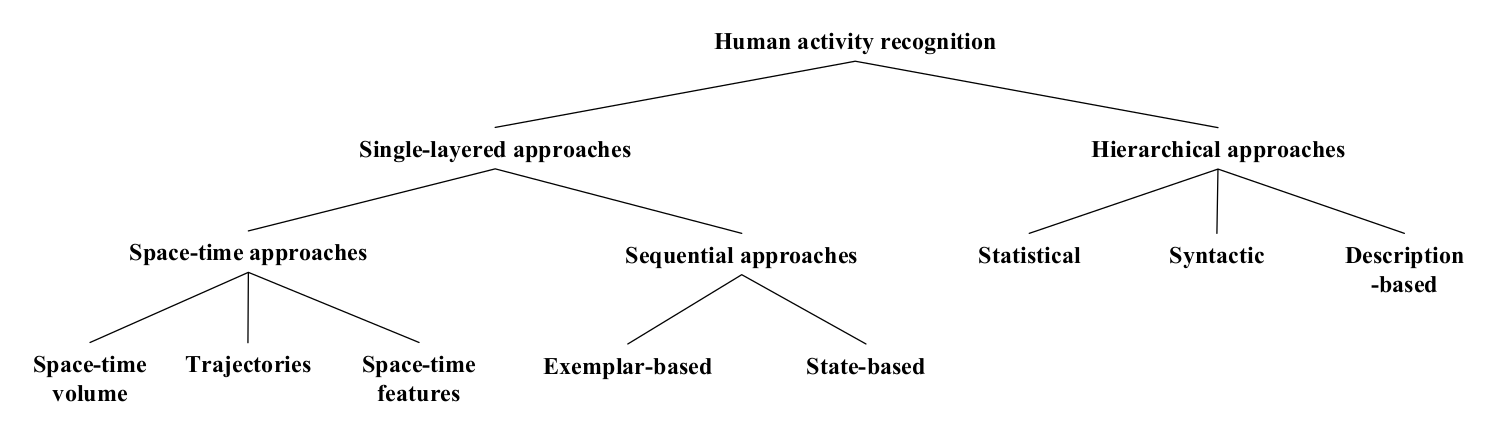
\includegraphics[width=\textwidth]{img_conventional/taxonomy_conventional_methods.png}
    \caption{Approach-based taxonomy for conventional methods in human action recognition as given by Aggarwal and Ryoo \cite{aggarwal_human_2011}}
    \label{fig:conventional_taxonomy}
\end{figure}

\textcite{aggarwal_human_2011} divide the field of activity/action recognition into single-layered and hierarchical approaches.
\begin{description}
    \item[Single-layered Approaches] recognize an action by directly processing raw video-data, i.e.\ based on sequences of video frames.
    \item[Hierarchical Approaches] model an action as a sequence of explicitly defined and individually recognizable atomic sub-actions.
\end{description}

Single-layered approaches are further categorized into space-time approaches and sequential approaches.
\begin{description}
    \item[Space-time approaches] interpret a video as a 3D space-time volume, that results from stacking the individual video-frames along the temporal dimension.
    \item[Sequential approaches] interpret a video as a sequence of observations, i.e.\ feature vectors extracted from individual frames.
\end{description}


\subsection{Single-layered Space-Time Approaches}
Space-time approaches use the entire video volume for action recognition and can be distinguished by what kind of features they use from the volume \cite{aggarwal_human_2011}.
Space-time volume approaches utilize pixel values of the full video volume or parts of it directly for creating a representation of the video, which is then compared with other video volume representations.
Trajectory based approaches use motion trajectories of tracked points inside the volume for the recognition of actions contained in it.
Space-time feature approaches extract features around interest-points locally and aggregate them into a representation of the video volume.


\subsubsection{Action recognition using Space-Time Volumes}
A prototypical approach for action recognition with space-time volumes is described in \cite{aggarwal_human_2011} and uses template matching:
Given a similarity measure for video volumes, the algorithm constructs or selects video volumes template from the training dataset for each action class that has to be recognized.
The template video volumes then act as representations for the action classes.
When presented with a test-video, the algorithm constructs the representation for the new video and compares it to the stored training templates by using the similarity measure.
The action class, that corresponds to the most similar training template is selected as output class for the test-video.

Approaches in this category mainly differ by how a representation is built and how they are compared.
\textcite{bobick_recognition_2001} create templates from the raw video volumes by stacking the silhouettes of persons that perform an action into 2D images.
The resulting binary \textit{motion-energy image} and skalar-valued \textit{motion-history image}, as displayed in figure \ref{fig:spacetimevolumes_meimhi}, are then classified by template matching as described above.

\begin{figure}[h]
    \centering
    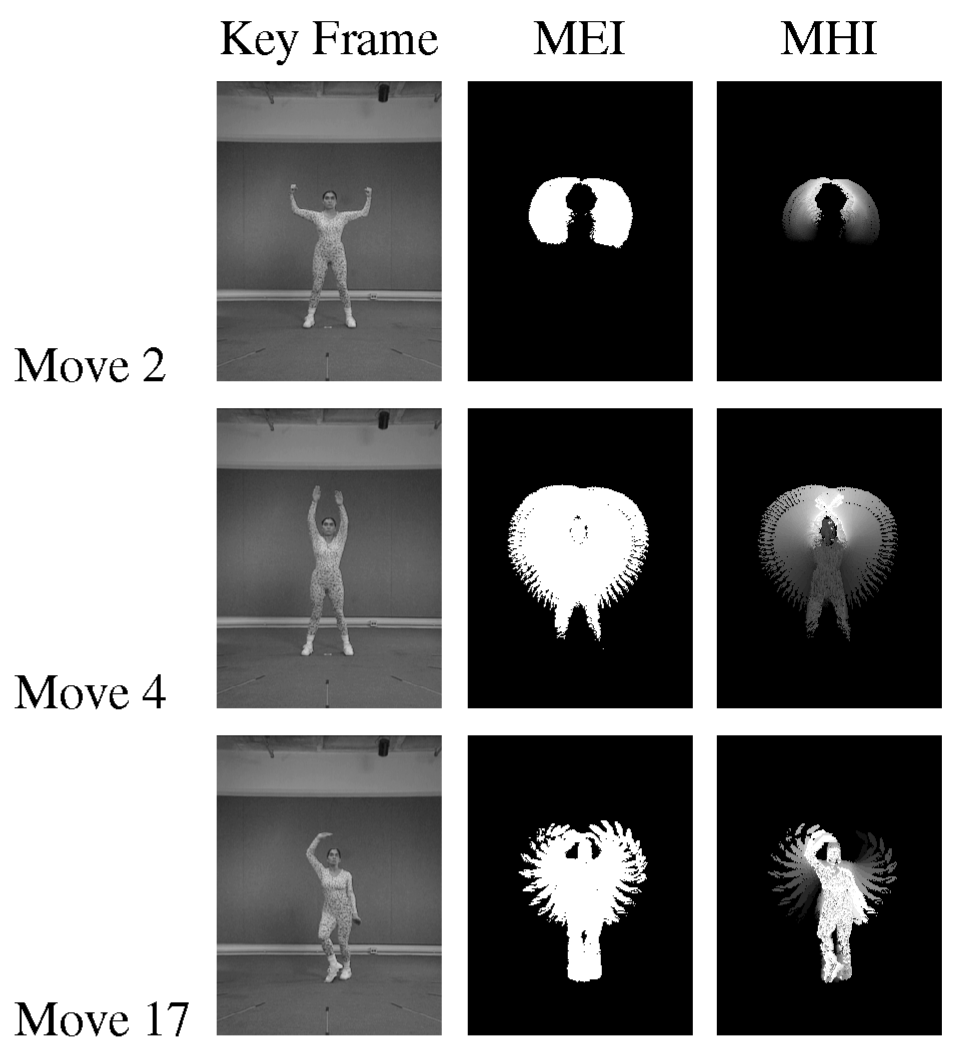
\includegraphics[width=.55\textwidth]{img_conventional/spacetimevolumes_meimhi}
    \caption{Motion-energy image (MEI), motion-history image (MHI) and example frame of three ballet actions \cite{bobick_recognition_2001}}
    \label{fig:spacetimevolumes_meimhi}
\end{figure}


\subsubsection{Action Recognition using Trajectories}
The underlying idea of trajectory-based approaches is, that the motion of a person's joint positions are sufficient for recognizing the performed action \cite{johansson_visual_1975}.
Algorithms that follow this approach use space-time trajectories to represent an action.
More specifically the joint positions of a person are tracked in the video volume.
The resulting trajectories then represent the performed action and can be used for classification, by either comparing the trajectories directly or by extracting features along the trajectories.

\textcite{sheikh_exploring_2005} classify actions by using the trajectories of $13$ tracked points directly as displayed in figure \ref{fig:trajectories_sheikh}.

\begin{figure}[H]
    \centering
    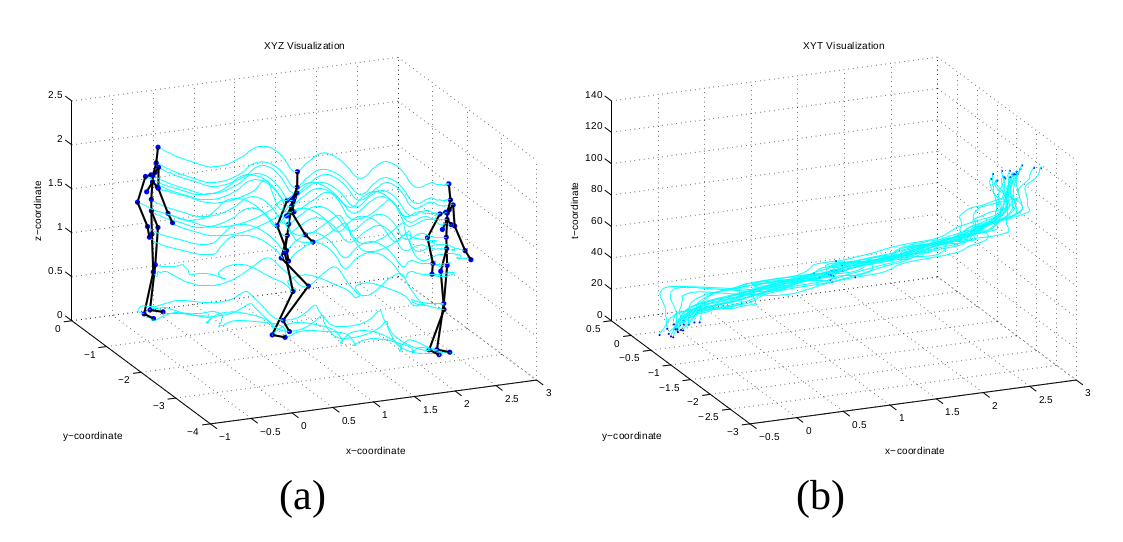
\includegraphics[width=\textwidth]{img_conventional/trajectories_sheikh}
    \caption{Trajectories of a person's tracked joint positions while performing an action. Trajectories shown in XYZ space (a) and XYT space (b) \cite{sheikh_exploring_2005}}
    \label{fig:trajectories_sheikh}
\end{figure}


\subsubsection{Action Recognition using Local Spatio-Temporal Features}
The principle idea behind action recognition with local spatio-temporal features is, that each action produces characteristic changes of pixel values in local 3D regions of the video containing the action \cite{poppe_survey_2010}.
Algorithms can therefore recognize actions by learning the correspondence between an action class and the set of the local regions, that are produced by the class.
A region, that contains these characteristic changes in pixel values, corresponds to a location in the video and is called a \textit{local spatio-temporal feature} or a \textit{spatio-temporal interest point}.
\textcite{aggarwal_human_2011} use the terms interchangeably.

\textcite{poppe_survey_2010} defines spatio-temporal interest points as regions in a video, where sudden changes in motion appear.
They note, that these regions are considered highly informative for action recognition and generally, points that perform a simple translation in the spatio-temporal video volume do not produce a local spatio-temporal feature.

More specifically, \textcite{schuldt_recognizing_2004} define a local space-time feature as ``primitive events corresponding to moving two-dimensional image structures at moments of non-constant motion''.

%In local spatio-temporal feature approaches, a video is generally treated as a 3D space-time volume, which results from stacking the individual video-frames.
%Local regions of characteristic motion are detected in this spatio-temporal volume, which can be interpreted as a three-dimensional object.

In general, a local spatio-temporal feature approach for action recognition contains three main aspects: \cite{karpathy_large-scale_2014}\cite{aggarwal_human_2011}
\begin{enumerate}
    \item \textbf{Feature Extraction}: Determining what kind of features, i.e.\ changes in pixel values, are considered as characteristic for the ongoing motion and where they are located. Feature extractors are specifically hand-crafted to best capture local motion information.
    \item \textbf{Feature Encoding}: Creating a fixed-sized representation of a video using the extracted local spatiotemporal features.
    \item \textbf{Classification}: Learns the correspondence between the video representations and the action class it contains.
\end{enumerate}

Feature extraction can be further divided into interest-point detection and local description \cite{poppe_survey_2010}.
Interest point detectors find and locate the locations of non-constant, informative motion.
Local descriptors transform the raw pixel values in neighbourhoods around previously detected interest points, to best capture the inherent motion information. 

A comparative evaluation of different interest point detectors and local descriptors was published in 2009 by \textcite{wang_evaluation_2009}.
They found, that instead of using computationally expensive feature detectors, dense sampling of interest points from the video is a well performing alternative. 

Prototypical approaches using local features were proposed by \textcite{laptev_space-time_2005} and \textcite{dollar_behavior_2005}.
\textcite{laptev_space-time_2005} extended the Harris corner and edge detector \cite{harris_combined_1988} for extracting space-time interest points in videos.

\begin{figure}[H]
    \centering
    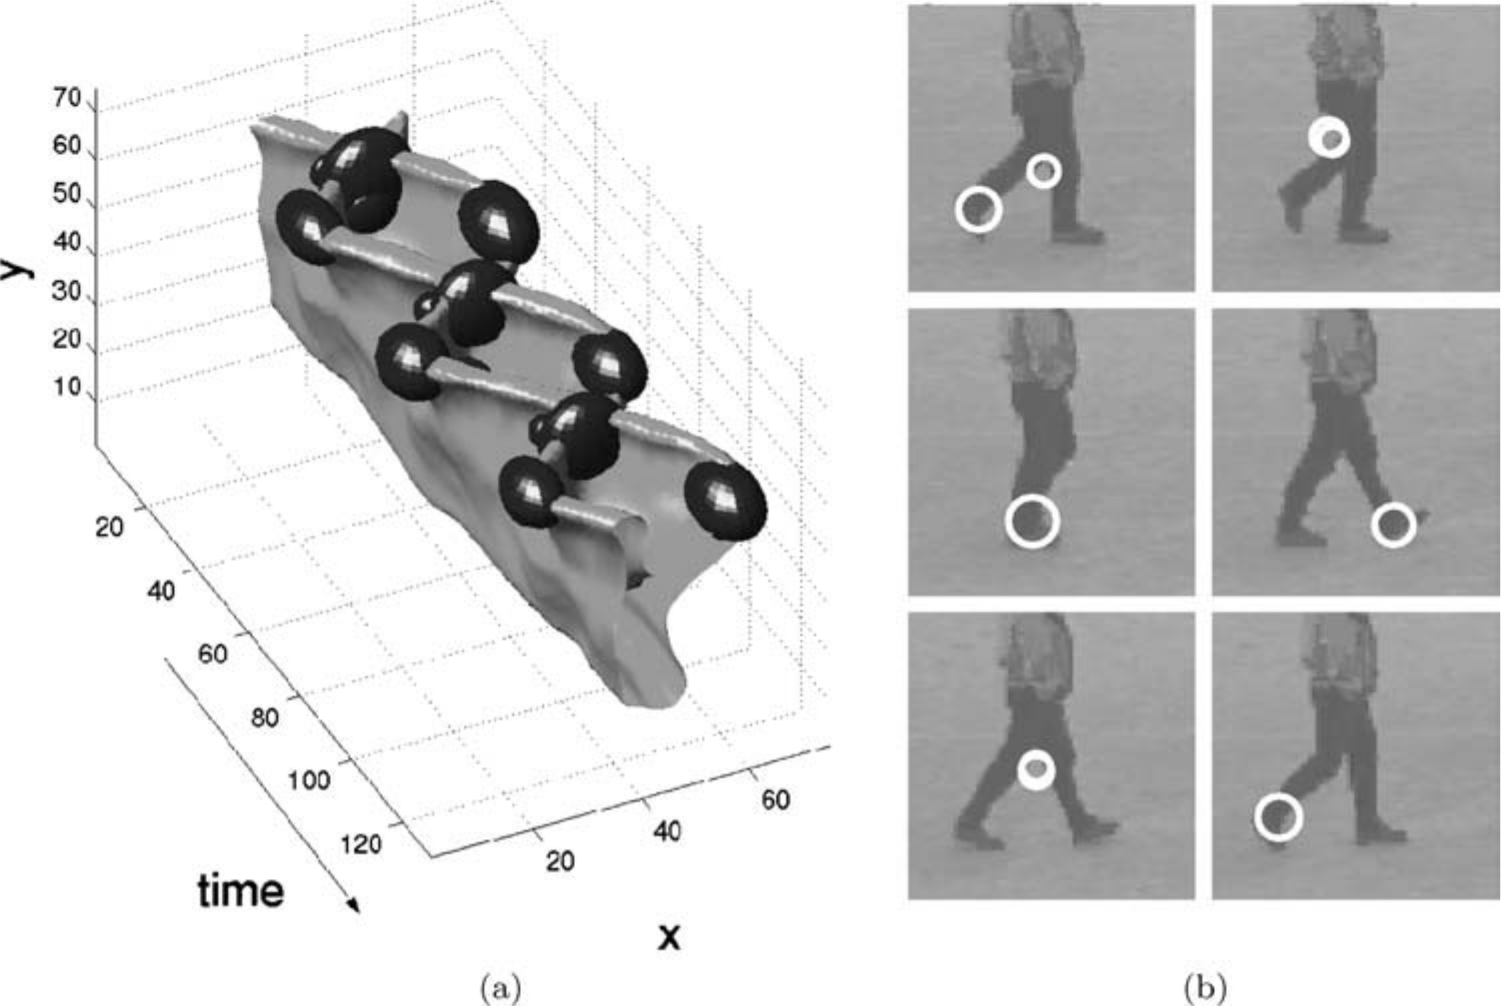
\includegraphics[width=.8\textwidth]{img_conventional/laptev_stip}
\caption{Detection of spatio-temporal interest points from the movement of legs. \textit{a}) Walking pattern of the legs (presented upside down) along with detected interest points (black ellipsoids). \textit{b}) Positions of detected interest points, projected into the original video. \cite{laptev_space-time_2005}}
    \label{fig:laptev_stip}
\end{figure}

\textcite{dollar_behavior_2005} proposed a feature detector for detecting periodic motions.
Once a spatio-temporal interest point is detected, a cube of video pixels called a \textit{Cuboid} as shown in figure \ref{fig:dollar_cuboids} is assigned to each detected point.
The local appearance information in each cube is then extracted and aggregated into a global video description.
They found, that motion information in the cuboids is best captured by transforming each into a flattened vector of brightness gradients to form the final local feature.
Given a training dataset, these final local features in the form of several vectors for each video, are extracted and a codebook of feature vectors is formed by using k-means.
Applying to the bag-of-words paradigm, a video is represented as a histogram of codeword frequencies given the codebook.
Specifically, at first the feature vectors are extracted from a video, each vector is then assigned to its nearest codebook feature vector, which is called a visual word.
By counting the number of visual word occurrences, a histogram representation of the video is created.
A classifier then learns the correlation between histogram representations and action labels.
This approach ignores the spatio-temporal relations between detected interest points.

\begin{figure}[H]
    \centering
    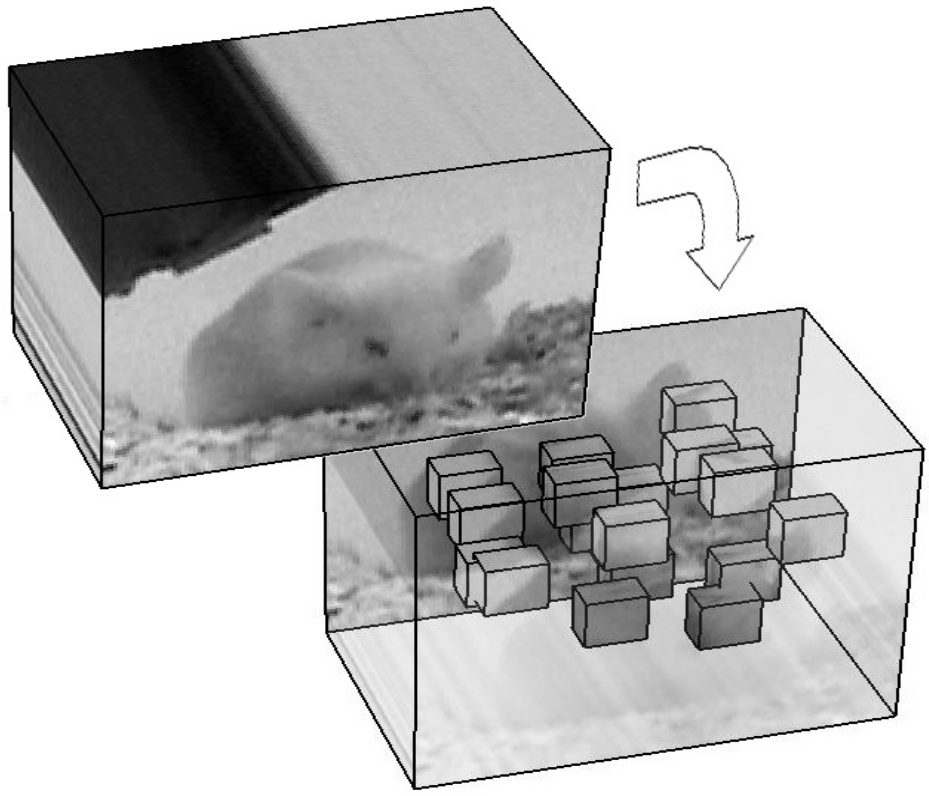
\includegraphics[width=0.4\textwidth]{img_conventional/dollar_cuboids}
    \caption{\cite{dollar_behavior_2005}}
    \label{fig:dollar_cuboids}
\end{figure}

Further examples of feature detectors are given in \cite{poppe_survey_2010}.

Beyond using the bag-of-words paradigm for encoding local features into a global video representation, other more advanced methods were proposed such as the Fisher Vector\cite{perronnin_fisher_2007} and the Vector of Locally Aggregated Descriptors (VLAD) \cite{jegou_aggregating_2010}.
An empirical evaluation of different encoding methods is given in \cite{peng_bag_2014}.

%Laptev and Lindeberg [26] proposed spatio-temporal interest points (STIPs)
%by extending Harris corner detectors to 3D. SIFT and HOG
%are also extended into SIFT-3D [34] and HOG3D [19] for
%action recognition. Dollar et al. proposed Cuboids features
%for behavior recognition [5]. Sadanand and Corso built Ac-
%tionBank for action recognition [33]. Recently, Wang et al.
%proposed improved Dense Trajectories (iDT) [44] which is
%currently the state-of-the-art hand-crafted feature. Tran 2015
%
%Recently, interest point detectors and local descriptors have
%been extended from images to videos. Laptev and Linde-
%berg [13] introduced space-time interest points by extend-
%ing the Harris detector. Other interest point detectors in-
%clude detectors based on Gabor filters [1, 5] or on the de-
%terminant of the spatio-temporal Hessian matrix [33]. Fea-
%ture descriptors range from higher order derivatives (local
%jets), gradient information, optical flow, and brightness in-
%formation [5, 14, 24] to spatio-temporal extensions of image descriptors, such as 3D-SIFT [25], HOG3D [11], extended
%SURF [33], or Local Trinary Patterns [34]. Action Recognition by dense trajectories -- Wang 2011


\subsection{Single-layered Sequential Approaches}
In single-layered sequential approaches an action is processed as a sequence of observations, specifically as a sequence of extracted feature vectors \cite{aggarwal_human_2011}.
As a first step in sequential approaches, feature vectors need to be extracted from each frame in the video that contains the action.
\textcite{aggarwal_human_2011} describe an example of using degrees of joint-angles as suitable feature vectors to describe the status of a person while performing an action.
Given the sequence of feature vectors from in input video, sequential approaches usually calculate the likelihood of action classes producing this observed sequence of feature vectors.
The action class with the highest likelihood is assigned to the input video.

\textcite{aggarwal_human_2011} further differentiate sequential approaches into exemplar-based and state model-based approaches.


\subsubsection{Exemplar-based Approaches}
Exemplar-based approaches store template sequences of feature vectors for each action class \cite{aggarwal_human_2011}:
A presented unknown action in an input video is recognized, by comparing its sequence of feature vectors to the stored templates.
The action class, whose template is most similar to the feature sequence of the input video is assigned to the input.
The approach has to take into account, that the feature sequences may vary because of different execution styles of action among different persons.

The Dynamic Time Warping algorithm (DTW) has been used widely for matching varying sequences in sequential exemplar-based approaches \cite{darrell_space-time_1993}\cite{gavrila_towards_1995}\cite{veeraraghavan_function_2006}.
Following figure \ref{fig:exemplar_dtw} illustrates the concept.

\begin{figure}[H]
    \centering
    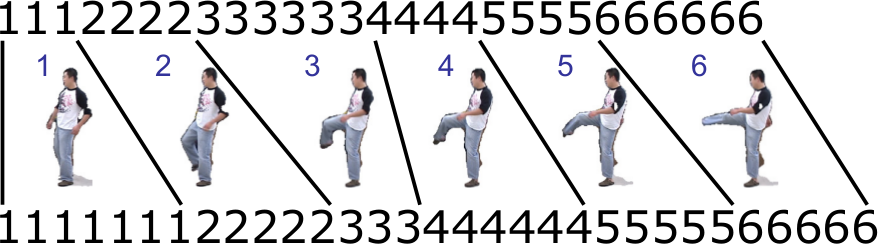
\includegraphics[width=0.6\textwidth]{img_conventional/exemplar_dtw}
    \caption{Matching of two action sequences with different execution rates. Each number corresponds to a pose of the person \cite{aggarwal_human_2011}}
    \label{fig:exemplar_dtw}
\end{figure}

\subsubsection{State Model-based Approaches}
In contrast to representing an action as a sequence of observations, state model-based approaches train one statistical model for each action class and an action is represented as a sequence of the model's hidden states \cite{cheng_advances_2015}.
Using the training videos of an action class, a model is trained on the extracted feature vector observations, so that it generates sequences of feature vectors corresponding to the class.
Given a test video, the likelihood of each model generating this sequence is calculated.
The class, that corresponds to the model with the highest likelihood, is assigned to the test video.
Hidden Markov Models and Dynamic Bayesian Networks have been used for these approaches \cite{aggarwal_human_2011}.


\subsection{Hierarchical Approaches}
The main idea of hierarchical approaches is to model complex actions as a hierarchy of simpler sub-actions \cite{aggarwal_human_2011}.
Sub-actions themselves can be further decomposed, until the initial complex action is represented as a sequence of non-decomposable atomic sub-actions.
A complex action is interpreted as a process that generates sub-actions which can be observed and classified individually.
Most hierarchical approaches thereby employ non-hierarchical single-layered action recognition approaches to recognize low-level sub-actions.

\textcite{aggarwal_human_2011} further differentiate hierarchical approaches into statistical approaches, syntactic approaches and desciption-based approaches.


\subsubsection{Statistical Approaches} 
Hierarchical statistical approaches use hierarchically stacked state-based models such as Hidden Markov Models (HMMs) \cite{oliver_layered_2002}\cite{zhang_modeling_2004} or Dynamic Bayesian Networks (DBNs) \cite{dai_group_2008}\cite{gong_recognition_2003} for action recognition.
Typically two layers of such models are used, where the bottom layer recognizes simple actions from sequences of feature vectors and the top layer recognizes high-level actions from the resulting sequence of simple actions.
The layered Hidden Markov Model approach of \textcite{oliver_layered_2002} is said to be one of the most fundamental forms of hierarchical statistical approaches \cite{aggarwal_human_2011}.


\subsubsection{Syntactic Approaches} 
In hierarchical syntactic approaches, a high-level action is represented as a string of symbols \cite{cheng_advances_2015}.
Each symbol therein corresponds to a simpler, possibly atomic, sub-action as described previously.
Equivalently to hierarchical statistical approaches, syntactic approaches require the recognition of sub-actions by using any of the previously described methods in order to obtain the string of symbols.
An action class is represented as a set of production rules from context-free grammars or stochastic context-free grammars \cite{ivanov_recognition_2000}\cite{moore_recognizing_2002}\cite{minnen_expectation_2003}\cite{joo_attribute_2006}, that generate sequences of symbols corresponding to the action class.
Syntactic approaches then use parsing techniques from the field of programming languages \cite{hopcroft_introduction_1979} to recognize high-level actions.


\subsubsection{Description-based Approaches}
The definition of description-based approaches by \textcite{aggarwal_human_2011} states: ``A description-based approach is a recognition approach, that explicitly maintains human activities' spatio-temporal structure.''
High-level actions are represented by occurrences of their underlying sub-actions, while temporal, spatial and logical relationships between the sub-actions are explicitly specified.
The temporal relations between sub-actions are usually specified by associating a time interval with an occurring action.
\textcite{allen_maintaining_1983}\cite{allen_actions_1994} introduced seven predicates to describe temporal relations between time intervals: \textit{before, meets, overlaps, during, starts, finishes} and \textit{equals}, which have been widely used for hierarchical description-based approaches \cite{pinhanez_human_1998}\cite{siskind_grounding_2001}\cite{nevatia_hierarchical_2003}\cite{ryoo_recognition_2006}.


\subsection{State of the Art Approaches using Local Features}
\label{subsec:conventionalsota}

\textcite{wang_action_2013} introduced the \textit{Improved Dense Trajectories} approach, which is often considered state of the art in action recognition using hand-crafted local features \cite{tran_learning_2015}\cite{wang_towards_2015}\cite{simonyan_two-stream_2014}.
Using the categorization proposed by the taxonomy of \textcite{aggarwal_human_2011}, it can be seen as a hybrid approach of being trajectory-based and using hand-crafted local features.The principle idea behind \textit{Improved Dense Trajectories} is to densely sample spatio-temporal interest points, tracking them using optical flow and extracting local hand-crafted features in regions around the resulting point trajectories.

A basic version of the approach, called \textit{Dense Trajectories}, was first published in 2011 \cite{wang_action_2011} and later improved in 2013 (\textit{Improved Dense Trajectories}) \cite{wang_action_2013}.

A comparison of hand-crafted feature approaches to recent deep learning methods in action recognition is given in section \ref{sec:evaluation}.
Beyond \textit{Improved Dense Trajectories}, the following approaches have been considered state of the art \cite{wang_towards_2015}\cite{lan_beyond_2015}and are compared as well:
\begin{itemize}
    \item Multi-view super vector for action recognition (2014) \cite{cai_multi-view_2014}
    \item Beyond Gaussian pyramid: Multi-skip feature stacking for action recognition (2015) \cite{lan_beyond_2015}
\end{itemize}

\subsubsection{Action Recognition by Dense Trajectories (2011)}
\textcite{wang_action_2011} introduce a tracking technique called \textit{dense trajectories} for action classification from videos.
Points are sampled densely from each frame and then tracked using a dense optical flow field.
Local spatio-temporal features are extracted in regions around the resulting point trajectories to form trajectory descriptors, which are then aggregated into a global video descriptor using the bag-of-words paradigm.

%
%Dense sampling of interest points has shown to yield improved performance in action recognition over sparse spatio-temporal interest points \cite{wang_evaluation_2009}.
%However using the KLT tracker to obtain dense trajectories or matching SIFT features on densely sampled points would be computationally too expensive to handle large datasets. 
%The authors approach therefore represents an efficient way to extract dense trajectories.

Since motion in a video, and therefore also the resulting trajectories, can stem from either motion of interest or unwanted camera motion, the authors propose using a descriptor called \textit{Motion Boundary Histogram} (MBH), which aims at focussing on foreground motion.
The MBH descriptor is designed to make the classification of actions in a video invariant to camera motion.

The overall approach for obtaining a descriptor along densely extracted trajectories is shown in figure \ref{fig:densetrajectories_approach}

\begin{figure}[H]
    \centering
    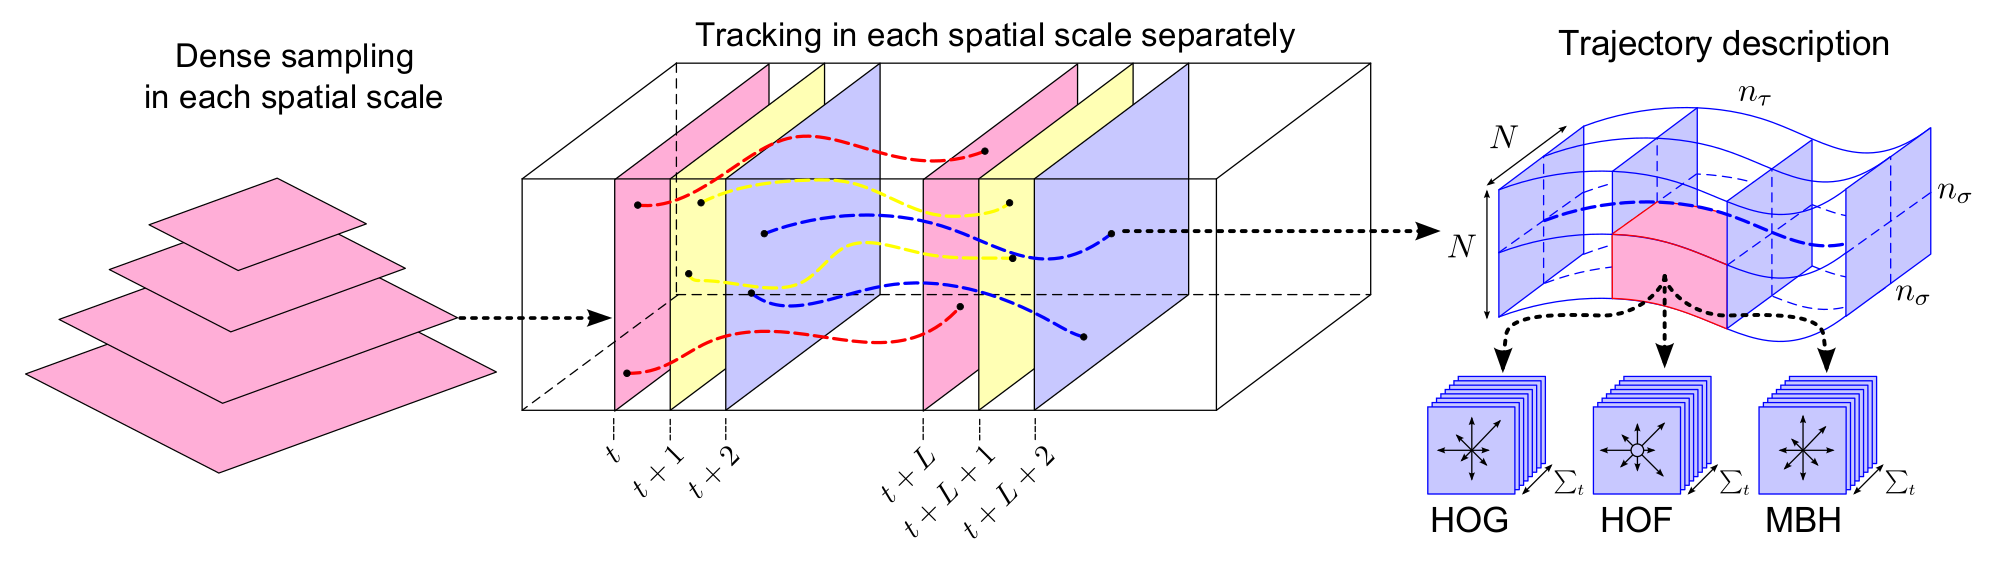
\includegraphics[width=\textwidth]{img_conventional/densetrajectories_approach}
    \caption{Description of densely extracted trajectories \cite{wang_action_2011}}
    \label{fig:densetrajectories_approach}
\end{figure}

Dense trajectories are obtained separately from 8 spatial scales, which differ by a factor of $1 / \sqrt{2}$.
Points are sampled on a grid spaced by $W$ pixels on each scale. Experimentally $W = 5$ has been shown to yield good results.
Each point $P_t$ at frame $t$ is tracked to the next frame by using a dense optical flow field, which was extracted by the Farnebäck algorithm \cite{farneback_two-frame_2003} as implemented in OpenCV.
%The tracked points in subsequent frames then form the trajectory $(P_t, P_{t+1}, P_{t+2}, \cdots)$.
%The maximum length of a trajectory is limited to $L = 15$ frames to avoid the problem of drifting.
%Trajectories that exceed this limit are removed from the tracking process.
%The presence of a trackectory in each $W \times W$ unit of each frame is verified. If no tajectory is present, a new point is sampled and added to the tracking process.

Since only dynamic information is important for action recognition, static trajectories are removed in a pre-processing stage.
Erroneous trajectories with sudden large displacements are also removed.

A simple descriptor is obtained from the shape of a trajectory itself.
It is formed by normalizing the spatial displacements given by the differences of consecutive points in a trajectory.
Formally the \textit{trajectory descriptor} $S'$ is given by:
\begin{equation*}
    S' = \frac{(\Delta P_t, \cdots, \Delta P_{t+L-1})}{\sum_{j=t}^{t+L-1} \|P_j\|}
\end{equation*}
Where $\Delta P_t = (P_{t+1} - P_t) = (x_{t+1} - x_t, y_{t+1} - y_t)$.

\textbf{Local Feature Descriptors:}\\
Local features are extracted from video volumes of size $N \times N \times L$ around the trajectories as depicted in figure \ref{fig:densetrajectories_approach}, where $N = 32$ has shown to yield good results.

Feature descriptors evaluated in the context of dense trajectories are):
\begin{itemize}
    \item \textbf{HOG} (Histogram of Oriented Gradients) \cite{dalal_histograms_2005-1}
    \item \textbf{HOF} (Histogram of Optical Flow) \cite{laptev_learning_2008}
    \item \textbf{MBH} (Motion Boundary Histogram) \cite{dalal_human_2006}
\end{itemize}

\begin{figure}[H]
    \centering
    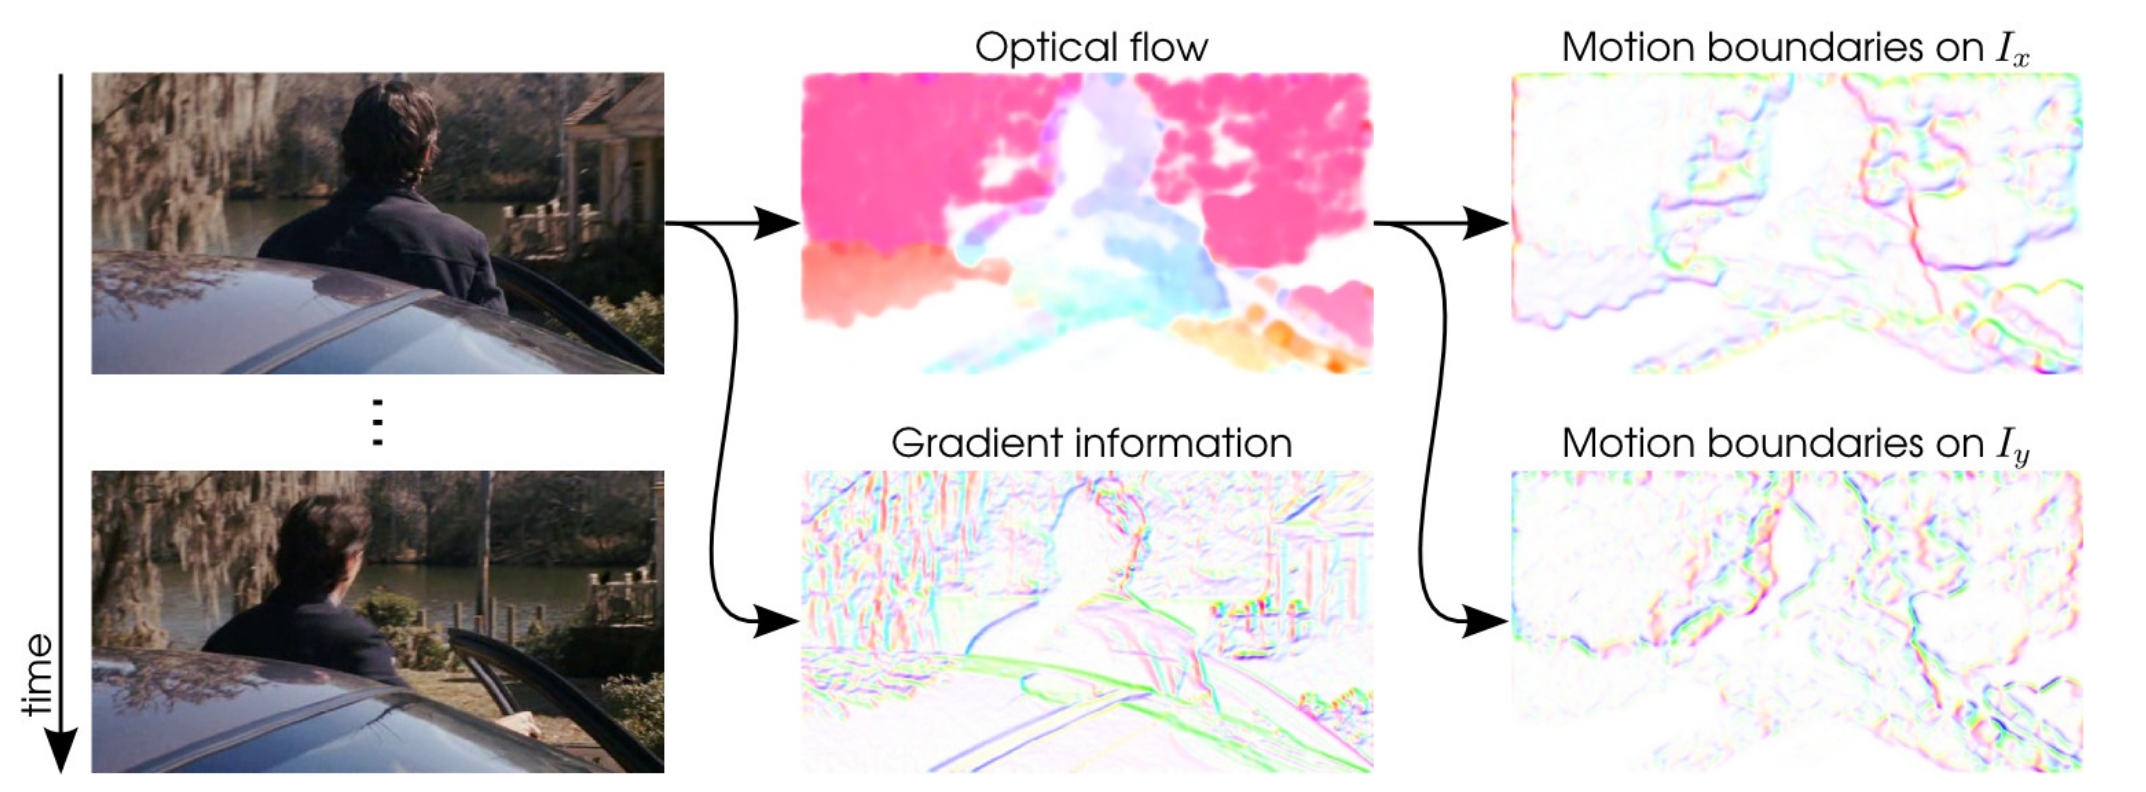
\includegraphics[width=\textwidth]{img_conventional/densetrajectories_featurevisualization}
    \caption{Visualization of the information captured by HOG, HOF and MBH on complete video frames. In each image, the orientation is given by color, the magnitude is given by saturation. \cite{wang_action_2011}}
    \label{fig:densetrajectories_featurevisualization}
\end{figure}

The HOG descriptor encodes static appearance information by computing the orientations of image gradients and aggregating them in a histogram over all subframes of the current video volume along the trajectory. In this approach the histograms contain 8 bins.

The HOF descriptor aggregates the orientations of optical flow vectors in a histogram and therefore captures local motion information. An additional bin is used here, i.e.\ 9 bins.

The MBH descriptor separately calculates the spatial derivatives of the $x$- and $y$-component of the optical flow field.
The orientations of the derivatives are aggregated into histograms (similarly to the HOG descriptor), which represent the video volume.
An advantage of MBH is that is suppresses constant motion, since it takes only the changes in the flow field (i.e.\ motion boundaries) into account.
The authors therefore use MBH as an easy way to filter noise stemming from background camera-motion, as can be seen by comparing the optical flow-image and motion boundaries in figure \ref{fig:densetrajectories_featurevisualization}.

The authors evaluate their approach on the KTH, YouTube, Hollywood2 and UCF-Sports dataset using a standard bag-of-features approach as follows:

\begin{enumerate}
    \item Construction of a codebook for each descriptor-type (trajectory, HOG, HOF and MBH).
        $100.000$ descriptors for each type are randomly chosen from all extracted descriptors over the training split.
        These descriptors are clustered into a 4000 words long codebook using $k$-means.
    \item Each extracted descriptor from a video is assigned to its nearest codebook-descriptor using the Euclidean distance.
        The number of occurrences are aggregated in a histogram, which builds the global video descriptor.
    \item A classifier (here a non-linear SVM with a $\chi^2$ kernel) is trained to assign the class-labels to the global video descriptors.
\end{enumerate}

Besides densely sampled trajectories, the authors evaluate baseline trajectories obtained from the KLT tracker for comparison.
The same descriptors (trajectory, HOG, HOF and MBH) are used around the KLT-trajectories.

\begin{table}[H]
    \centering
    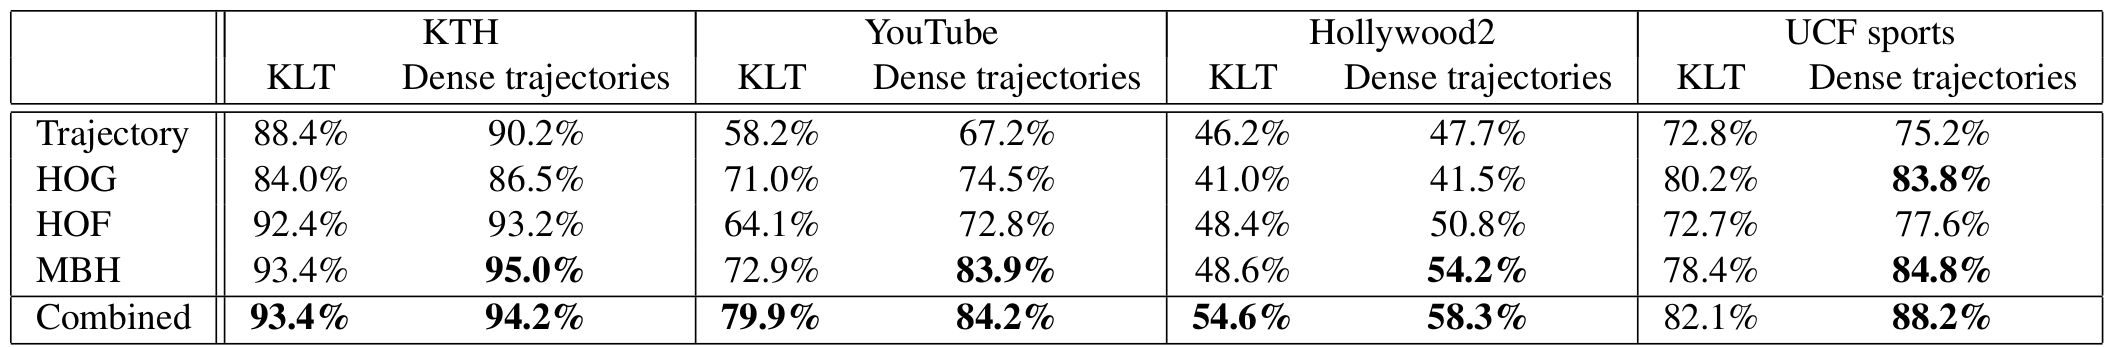
\includegraphics[width=\textwidth]{img_conventional/densetrajectories_results}
    \caption{Results of dense trajectories compared to KLT-trajectories when using different feature descriptors. \cite{wang_action_2011}}
    \label{tab:densetrajectories_results}
\end{table}

Other approaches used feature trajectories for action recognition by either tracking sparse spatio-temporal interest points using a standard KLT tracker \cite{lucas_iterative_1981} or by matching SIFT features \cite{lowe_distinctive_2004} between consecutive frames.
The results in table \ref{tab:densetrajectories_results} show the superiority of dense trajectories compared to the KLT baseline.
The simple trajectory descriptor yields surprisingly good results, which according to the authors confirms the importance of motion information encoded in the trajectory shapes themselves.
The MBH descriptor performs significantly better than all the other descriptors.
On the YouTube dataset, the advantage of using the MBH descriptor is most prominent, since the videos in this dataset contain a lot of noise from camera-motion (uncontrolled, realistic videos, often recorded by handheld cameras).


\subsubsection{Action recognition with improved trajectories (2013)}
TODO
\cite{wang_action_2013}
``Recently, Wang et al. proposed improved Dense Trajectories (iDT) [44] which is currently the state-of-the-art hand-crafted feature'' tran learning spatio-temporal features with 3D convolutional networks.

\section{Deep Learning Methods in Action Recognition}
META: Review of approaches that use Deep Learning methods.

Taxonomy of approaches.


\subsection{3D-Convolutional Networks}
I.e. convolutional methods.

The naive approach: using framewise information, classifying it with a CNN and average the results. Elaborate further\ldots ??

``Video analysis provides more information to the recognition task by adding a temporal component through which motion and other information can be additionally used. At
the same time, the task is much more computationally de-
manding even for processing short video clips since each
video might contain hundreds to thousands of frames, not
all of which are useful. A naive approach would be to treat
video frames as still images and apply CNNs to recognize
each frame and average the predictions at the video level.
However, since each individual video frame forms only a
small part of the video’s story, such an approach would
be using incomplete information and could therefore eas-
ily confuse classes especially if there are fine-grained dis-
tinctions or portions of the video irrelevant to the action of
interest.'' Beyond Short Snippets: Deep Networks for Video Classification

explain: feature maps

Treated as an additional spatial dimension.


\subsubsection{3D Convolutional Neural Networks for Human Action Recognition (2010/2013)}

\textcite{ji_3d_2013} propose 3D convolutions for action recognition from video with convolutional neural networks (CNNs).
3D convolutions are able to process spatial as well as temporal information in a convolutional layer.

In regular 2D CNNs the convolutional layers apply 2D convolutional kernels to the previous layers to extract features from them.
More formally, in the notation of the authors, the value $v_{ij}^{xy}$ at spatial position $(x,y)$ of feature map $j$ in convolutional layer $i$ of the network is given by:
\begin{align*}
    v_{ij}^{xy} = \tanh \left( b_{ij} + \sum_m \sum_{p=0}^{P_i -1} \sum_{q = 0}^{Q_i - 1} w_{ijm}^{pq} v_{(i-1)m}^{(x+p)(y+q)} \right)
\end{align*}
The two inner sums over $p$ and $q$ carry out the convolutional operation on feature map $v_{(i-1)m}$ of the previous layer $i-1$ with the 2 dimensional convolutional kernel $w_{ijm}$ (spatial indices omitted).
Thereby $w$ is a tensor-like object, which contains all 2 dimensional convolutional kernels in the network, that produce feature maps through convolution
Specifically, $w_{ijm}^{pq}$ denotes the value at spatial positions $(p,q)$ of the 2D convolutional kernel, which is applied to feature map $m$ of the previous layer $i-1$.
Feature map $j$ in layer $i$ is finally obtained by summing the results of all the convolutions performed on the feature maps of layer $i-1$ over $m$, adding a bias and passing it into a non-linear function (here $\tanh(\cdot)$).

$P_i$ and $Q_i$ denote the dimensions of the kernels in $x$ and $y$-direction respectively.
The convolutional operation used here is called \textit{cross-correlation}, which differs from the mathematical discrete convolution in that the convolutional kernel is not flipped. This results in a non-commutative operation as described in chapter 9 of \cite{goodfellow_deep_2016}.

\textcite{ji_3d_2013} propose an extension of 2D convolutions by using three dimensional kernels, i.e.\ two spatial dimensions as above and an additional temporal dimension.
More formally the value $v_{ij}^{xyz}$ of feature map $j$ at spatio-temporal position $(x,y,z)$ in convolutional layer $i$ is given by:
\begin{align*}
    v_{ij}^{xyz} = \tanh \left( b_{ij} + \sum_m \sum_{p=0}^{P_i -1} \sum_{q = 0}^{Q_i - 1} \sum_{r = 0}^{R_i - 1} w_{ijm}^{pqr} v_{(i-1)m}^{(x+p)(y+q)(z+r)} \right)
\end{align*}
As above, $w_{ijm}^{pqr}$ denotes the value of the now three dimensional kernel at spatio-temporal position $(p,q,r)$, which performs convolution on the $m$th feature map of the previous layer $i-1$ to obtain feature map $j$ in convolutional layer $i$.
$R_i$ additionally denotes the dimension of the kernel in temporal direction. 

Based on 3D convolutions, the authors design a neural network architecture, that takes an input of $7$ video-frames of size $60 \times 40$ pixels.
The details of the architecture as shown in figure \ref{fig:3dconv_architecture} are described below:

\begin{figure}[H]
    \centering
    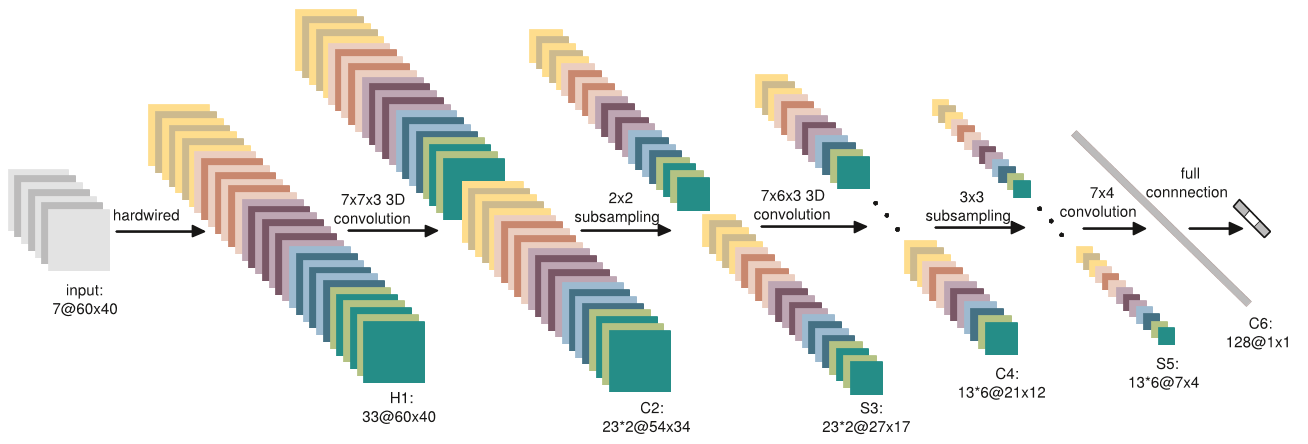
\includegraphics[width=\textwidth]{img_deep/3dconv_architecture}
    \caption{3D CNN architecture developed for human action recognition \cite{ji_3d_2013}}
    \label{fig:3dconv_architecture}
\end{figure}
The architecture contains one hard-wired layer, three convolutional layers \textit{C2, C4} and \textit{C6}, two subsampling layers for dimensionality reduction \textit{S3} and \textit{S5} and one fully connected layer for classification.

At first, hard wired connections are applied to the input frames, in order to extract gray values of the input frames, gradients along the horizontal and vertical direction and the optical flow between two consecutive frames. This results in 33 feature maps in layer $H1$, organized in five different channels: \textit{gray, gradient-x, gradient-y, optflow-x} and \textit{optflow-y}.

The first convolutional layer \textit{C2} applies two 3D kernels with dimesions $7\times7\times3$ ($7\times7$ pixels in the spatial dimension and $3$ frames in the temporal dimension) to each of the five channels in layer $H1$ separately. 
This results in $2\times5$ channels with a total of 46 feature maps in layer \textit{C2}.
The first convolutional layer therefore requires $\text{(kernel-weights)} + \text{(biases)} = 2 \times 5 \times 7 \times 7 \times 3 + 2 \times 5 = 1480$ trainable parameters. 

After subsampling layer \textit{S3}, three different 3D kernels with size $7 \times 7 \times 3$ are applied to each of the $2 \times 5$ channels of the previous layer to get the feature maps in layer \textit{C4}.
The last convolutional layer \textit{C6} performs 2D convolutions to obtain $128$ feature maps of dimension $1 \times 1$.

The resulting vector of these 128 feature maps in layer $C6$ is interpreted as a 128-dimensional feature representation of the input.
This feature representation is then classified by a fully connected layer into the required number of output classes.

In total the architecture contains $295,458$ trainable parameters, which are initialized randomly and learned by online error back-propagation as done by \textcite{lecun_gradient-based_1998-1}.
The authors tried other architectural layouts but conclude that the one described above works best.

The network is evaluated as part of an action detection and recognition system, using the TRECVID 2008 development dataset \cite{rose_trecvid_2009}.
Additionally, it's performance is measured as stand-alone approach on the KTH benchmarking datset \cite{schuldt_recognizing_2004}.

\textbf{Evaluation on TRECVID:} \\
The TRECVID 2008 development dataset \cite{rose_trecvid_2009} contains 49 hours of surveillance videos continuously recorded by five different cameras on five days at London Gatwick Airport.
The datset is annotated for surveillance event detection, i.e.\ what events occur where.
The authors train their model to recognize three action classes from the dataset: \textit{CellToEar}, \textit{ObjectPut} and \textit{Pointing}.
The other action classes provided by the dataset were used to generate negative training examples.
The distribution of training examples sorted by date is shown in figure \ref{fig:3dconv_dataset}.
Example frames of the datset are shown in figure \ref{fig:3dconv_sampletracking}.

\begin{figure}[H]
    \centering
    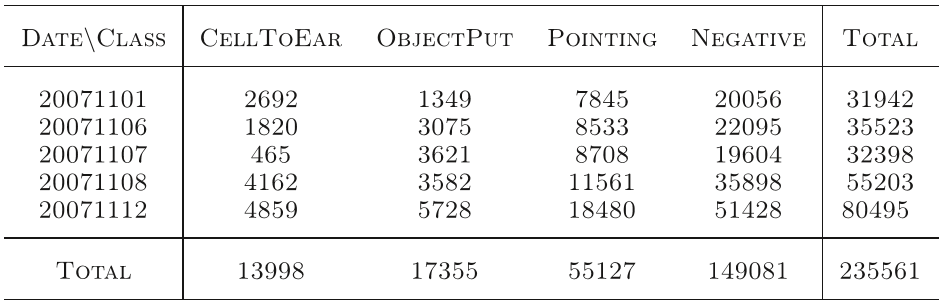
\includegraphics[width=0.75\textwidth]{img_deep/3dconv_dataset}
    \caption{Number of action samples per class from the TRECVID 2008 development dataset \cite{ji_3d_2013}}
    \label{fig:3dconv_dataset}
\end{figure}

Since the dataset provides continuous videos with several persons in a real-world scence, \textcite{ji_3d_2013} apply a human detector and a detection-driven tracker, to keep track of the heads in the scene.
This information is used to extract a bounding box around a person, as soon as an action is performed. 
Six additional bounding boxes are sampled from three frames before and three frames after the action was detected with a temporal step size of two frames.
The bounding boxes have the same size and are sampled at the same spatial location as the initial bounding box.

The contents of these 7 bounding boxes are stacked and used as input of the 3D CNN architecture in order to classify the performed action.

\begin{figure}[H]
    \centering
    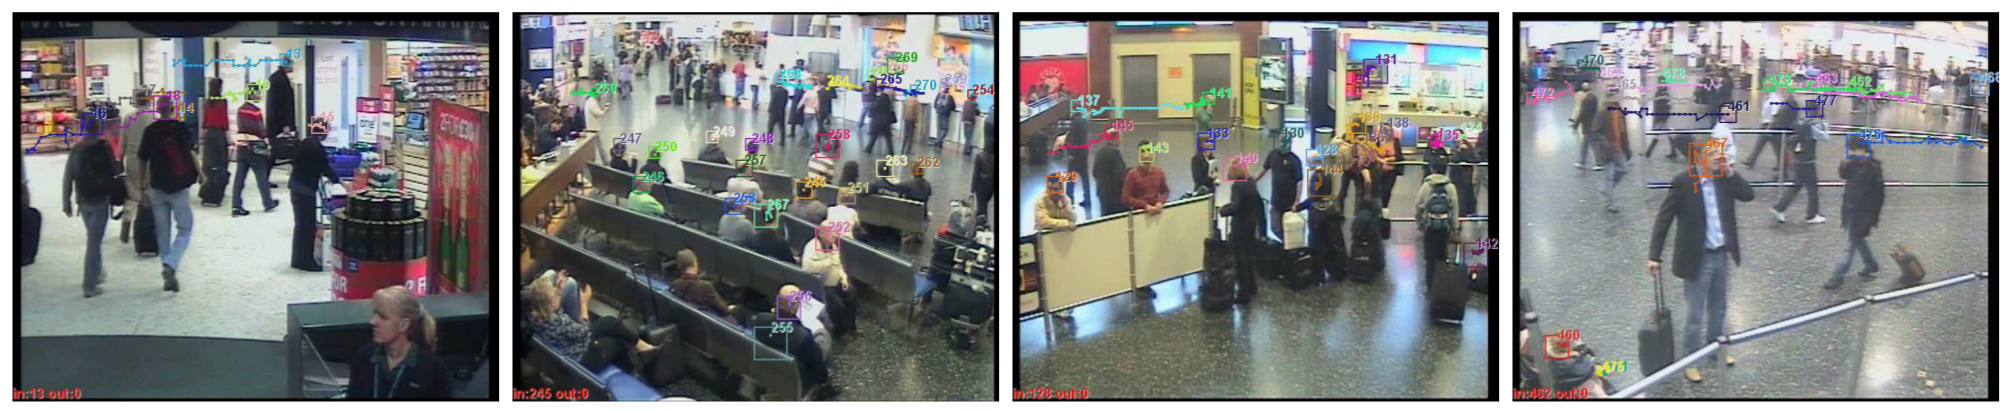
\includegraphics[width=\textwidth]{img_deep/3dconv_sampletracking}
    \caption{Example scenes of the TRECVID 2008 development dataset with results of human detection and tracking \cite{ji_3d_2013}}
    \label{fig:3dconv_sampletracking}
\end{figure}

To evaluate the performance of the 3D CNN model, the authors compare it to three other baseline approaches in the detection and recognition system:
\begin{enumerate}
    \item A frame-based 2D CNN model, which averages the action class predictions over individual frames.
    \item Extraction of dense SIFT features \cite{lowe_distinctive_2004} from the seven (grayscaled) input frames, which are then aggregated using the BoW-Paradigm and classified through a linear SVMs.
    \item Extraction of dense SIFT features \cite{lowe_distinctive_2004} from motion edge history images (MEHI)\cite{yang_human_2009} of the input frames, which are then aggregated as above.
\end{enumerate}

The 3D CNN model outperfoms the other approaches on the TRECVID 2008 development dataset significantly for all classes except \textit{Pointing}, where the 2D frame-based CNN performed best.
The authors note, that the number of training examples for \textit{Pointing} are significantly larger than for any other class and conclude, that their architecture performs best, when few positive examples are present.

\textbf{Evaluation on KTH:}\\
Furhermore, the stand-alone 3D CNN architecture was evaluated on the KTH dataset \cite{schuldt_recognizing_2004}.
It achieves an overall accuracy of $90.2\%$ on that benchmark.
In comparison: \textcite{schindler_action_2008} achieved $92.7\%$ and \textcite{jhuang_biologically_2007} achieved $91.7\%$ several years earlier.

\textcite{ji_3d_2013} showed, that 3D convolutions yield competitive performace compared to state-of-the-art approaches at that time as shown on the KTH benchmark \cite{schuldt_recognizing_2004}.
Although the authors reference the work of \textcite{schindler_action_2008} which states, that 5-7 video-frames are enough for recognizing simple actions, this short temporal extend is often identified as a deficit of the approach and addressed in following approaches, e.g.\ by \textcite{baccouche_sequential_2011}.


\subsubsection{Sequential Deep Learning for Human Action Recognition (2011)}
\textcite{baccouche_sequential_2011} identify two deficits of previous approaches for extending CNNs to the video domain, specifically the approach of 3D convolutions such as \cite{ji_3d_2013} and \cite{kim_human_2007}:
\begin{enumerate}
    \item They still rely on hand crafted inputs (hard wired pre-processing of the data to produce image gradients and optical flow in the first processing layer).
    \item The models typically process less than 15 input frames, and therefore only classify short sub-clips, not the entire video.
\end{enumerate}

To address these issues, the authors design a two-step deep architecture, which is shown in figure \ref{fig:sequentialdeep_overview} and consists of:
\begin{enumerate}
    \item A convolutional spatio-temporal feature extractor network, based on 3D convolutions.
    \item A recurrent neural network (RNN) classifier, which incorporates LSTM cells \cite{hochreiter_long_1997} to classify the entire sequence of previously extracted spatio-temporal features.
\end{enumerate}

\begin{figure}[H]
    \centering
    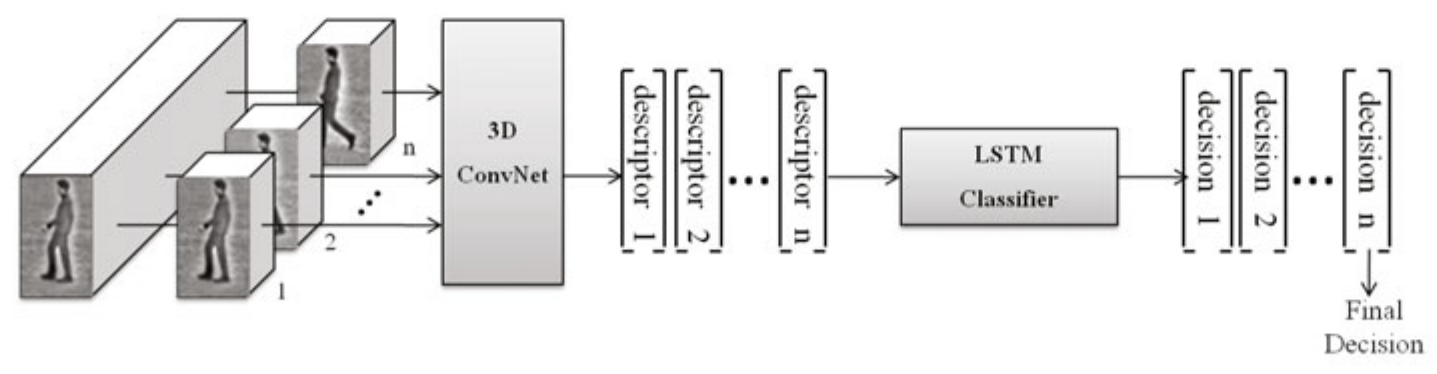
\includegraphics[width=\textwidth]{img_deep/sequentialdeep_overview.png}
    \caption{Overview of the two-step architecture consisting of a 3D ConvNet and a recurrent neural network classifier. \cite{baccouche_sequential_2011}}
    \label{fig:sequentialdeep_overview}
\end{figure}

\textcite{baccouche_sequential_2011} incorporate the work of \textcite{ji_3d_2013} by using a 3D ConvNet as feature extraction stage, which processes raw pixel values instead of hand-crafted inputs.
To compensate the problem of temporally short inputs and to take the temporal evolution of movements during an action into account, a RNN classifier is added, because they are able to process input sequences of arbitrary length.
The RNN classifies a sequence of feature representations, previously extracted by applying the 3D ConvNet to temporally adjacent patches of the input video, in order to recognize an action. 
Similarly to \cite{ji_3d_2013}, the overall approach is evaluated on the KTH dataset \cite{schuldt_recognizing_2004}.

Details of the 3D ConvNet architecture are shown in figure \ref{fig:sequentialdeep_cnnarchitecture}.
\begin{figure}[H]
    \centering
    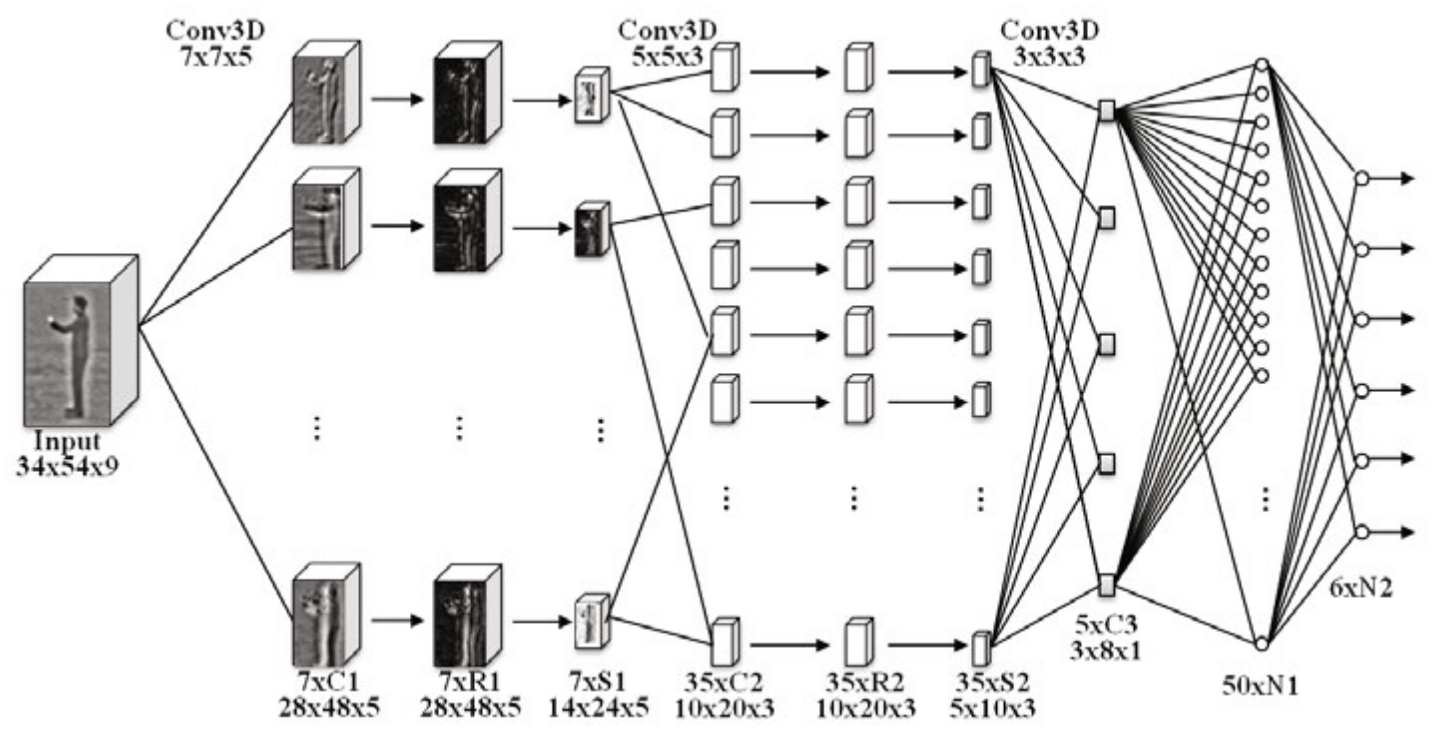
\includegraphics[width=0.9\textwidth]{img_deep/sequentialdeep_cnnarchitecture}
    \caption{Detailed architecture of the 3D ConvNet for later use with an RNN classifier. \cite{baccouche_sequential_2011}}
    \label{fig:sequentialdeep_cnnarchitecture}
\end{figure}

The input to the 3D ConvNet is formed by stacking $9$ successive frames from the input video of spatial resolution $34\times54$ pixels.
The network contains three convolutional layers \textit{C1, C2} and \textit{C3}.
The first two convolutional layers are followed by rectification and subsampling layers \textit{R1, S1} and \textit{R2, S2}.
A rectification layer simply computes the absolute value of its input \cite{baccouche_sequential_2011}.
The third convolutional layer is followed by two neuron layers (fully-connected layers) \textit{N1} and \textit{N2}.

The ConvNet model, as shown in figure \ref{fig:sequentialdeep_cnnarchitecture} embeds $17,169$ trainable parameters in total, which is about 15 times less than the $295,458$ parameters used by \textcite{ji_3d_2013}.

Specifically, the layers are configured as follows:
\begin{enumerate}
    \item Convolutional layer \textit{C1} computes $7$ feature maps, by convolving $7$ 3D $7\times7\times5$ kernels with the stacked input frames.
    \item Layer \textit{R1} and \textit{S1} perform rectification (building of the absolute value) and subsampling with a spatial factor of 2 respectively.
    \item Convolutional layer \textit{C2} computes $35$ feature maps (the $7$ feature maps in layer \textit{S1} are connected to two different convolutional kernels, which results in $14$ feature maps and pairs of different feature maps in \textit{S1} are connected to one convolutional kernel each, which results in additional $21$ feature maps, summing to a total of $35$ feature maps).
    \item Convolutional layer \textit{C3} computes $5$ features maps, which are fully connected to all feature maps in previous layer \textit{S2} by $3\times3\times3$ convolutional kernels. These five feature maps have dimension $3\times8\times1$, rendering the raw input encoded as a 120 dimensional feature vector.
\end{enumerate}

The 3D ConvNet is trained individually on the KTH dataset before employing the RNN classifier.
For training, the 120 dimensional feature vector is fed into two fully connected layers \textit{N1} and \textit{N2} with 6 output neurons, one for each class of the KTH dataset.
The authors use the same training algorithm as \textcite{ji_3d_2013}: online Backpropagation with momentum adapted to weight-sharing.

For training the RNN classifier with online backpropagation through time \cite{gers_learning_2002}, the fully connected layers \textit{N1} and \textit{N2} of the 3D ConvNet are removed.
The 120 output values of the third convolutional layer \textit{C3} are fed into the recurrent neural network as input at each time step.
Several configurations were tested by the authors and a single hidden layer with 50 LSTM cells were found to be a good compromise between training time and performance.
The LSTM cells are fully connected to the outputs of layer \textit{C3}.

The authors find their 3D ConvNet model alone, without adding the recurrent LSTM classifier, to yield a recognition rate of $91.04\%$ on KTH, when the classification is done by majority voting over several short sub-sequences of the test-video.
This result is comparable to other approaches at that time and almost the same as obtained by \textcite{ji_3d_2013} ($90.2\%$), although the model requires about 15 times less paramerters.
When using the LSTM classifier network, recognition performance increases to $92.17\%$.


\subsubsection{Large-scale Video Classification with Convolutional Neural Networks (2014)}
\textcite{karpathy_large-scale_2014} provide a comprehensive examination of techniques to apply convolutional neural networks to the domain of action recognition from video.
More specifically, their contribution is four-fold:
\begin{enumerate}
    \item They gather the Sports-1M dataset containing a collection of 1 million automatically annotated sports videos from YouTube (further described in section \ref{chap:datasets} of this work).
    \item They evaluate several approaches besides three dimensional convolutions for extending CNNs to process spatio-temporal data in a consistent and therefore comparable manner. These methods are called \textit{fusion methods} in the phrasing of the authors, since temporal motion information has to be fused with spatial motion information while propagating through a network.
    \item They propose a generic multiresolution convolutional architecture in oder to speed up training time at no cost in accuracy.
    \item They retrain the top layers of a network on the UCF-101 dataset, which has previously been trained on the Sports-1M dataset and thereby achieve a significant increase in performance against training the network on UCF-101 alone (transfer learning).
\end{enumerate}

The authors first implement a baseline CNN architecture, which classifies human action videos by processing a single frame at a time, i.e.\ without considering temporal relationship between frames.
Based on the single frame architecture, several extensions for processing temporal information in the network are being investigated. These types of fusion methods are depicted in figure \ref{fig:largescale_fusionmethods}.

\begin{figure}[H]
    \centering
    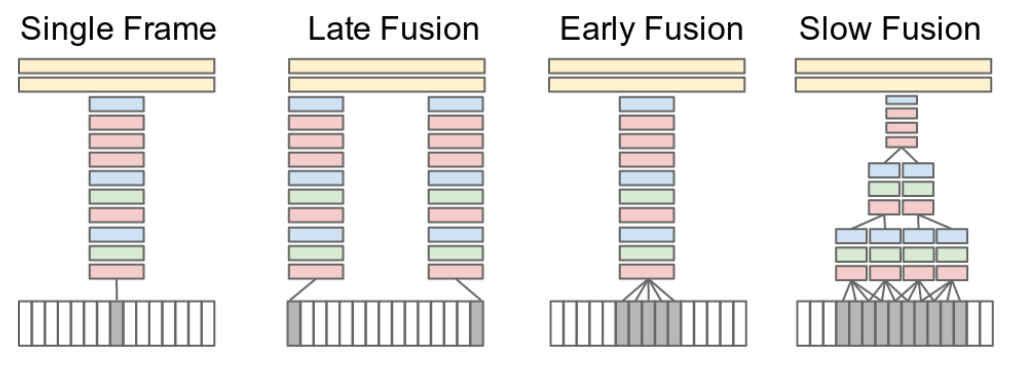
\includegraphics[width=0.75\textwidth]{img_deep/largescale_fusionmethods}
    \caption{Different methods for fusing temporal with spatial information in convolutional neural network architectures. Red, green and blue denotes convolutional, normalization and pooling-layers. Grey colored inputs are single RGB video frames. Yellow layers are fully-connected for classification. \cite{karpathy_large-scale_2014}}
    \label{fig:largescale_fusionmethods}
\end{figure}

\textbf{Single Frame}\\
The CNN model used in the single frame approach is a deep convolutional neural network with 2D convolutions, that recognizes actions by classifying frames of a given input sequence individually and reporting the averaged prediction.
The architecture is similar to AlexNet, which won the 2012 ImageNet Classification Challenge \cite{krizhevsky_imagenet_2012-1}, but receives slightly smaller inputs: $170\times170\times3$ instead of $224\times224\times3$ in the ImageNet model.
The first two dimensions thereby corresprond to the spatial resolution of the video, the third dimension to the RGB color channels of a video-frame.
This approach is evaluated as a baseline in order to measure the improvement when using temporal information, i.e.\ several frames, in the recognition process. 

\textbf{Early Fusion}\\
In the early fusion approach temporal information is incorporated in the network on the pixel level by extending the convolutional kernels in the first layer to be of dimension $11 \times 11 \times 3 \times T$, where $T$ is the temporal extend, i.e.\ the number of input frames to the network.
The authors set $T = 10$ which corresponds to a third of a second.
Note that the temporal information is completely flattened after the first convolutional layer, since the kernel has the same temporal dimension as number of inputs frames.
Therefore only the kernels in the first convolutional layer are three dimensional in nature.

\textbf{Late Fusion}\\
In the late fusion methods, two separate single-frame networks with shared parameters and without their individual classification layers are used on input frames with a temporal distance of $15$ frames.
Two shared fully connected layers then merge the individual network's information and classify the input. 
The fully connected layers are able to compute motion information by comparing the feature representations of the two single-frame networks.

\textbf{Slow Fusion}\\
Temporal information is processed throughout the network by extending the kernels of each convolutional layer in time, as done in the first layer of the \textit{Early Fusion} approach.
Thereby higher layers progressively process more temporal information along the input frames.
The \textit{Slow Fusion} approach applys 3D convolutions as done by \textcite{ji_3d_2013} and \textcite{baccouche_sequential_2011}.
The first convolutional layer incorporates a temporal extend of $T = 4$ in its kernels, while the second convolutional layer uses a temporal extend of $T = 2$.
This allows the third convolutional layer layer to access the information of all 10 input frames.

\textbf{Evaluation on the Sports-1M dataset}\\
The recognition performance of the different fusion methods is evaluated on the Sports-1M dataset.
The authors use downpour stochastic gradient descent \cite{dean_large_2012} for training the models in a distributed way on a computing cluster.
For the evaluation $70\%$ of the dataset were used as training data, $10\%$ as validation set and $20\%$ as test set.

To obtain fixed-sized inputs for the models, the authors interpret an entire video as a set of short, fixed-sized video clips.
At test time, 20 short clips are sampled from the current test-video and each clip is presented to the network individually.
Each clip is passed through the network 4 times, each time using different crops and flips and the result is averaged to produce a robust class prediction.
The video-level predictions (examples shown in figure \ref{fig:largescale_classification}) are computed from the clip-level predictions simply by averaging.

\begin{figure}[H]
    \centering
    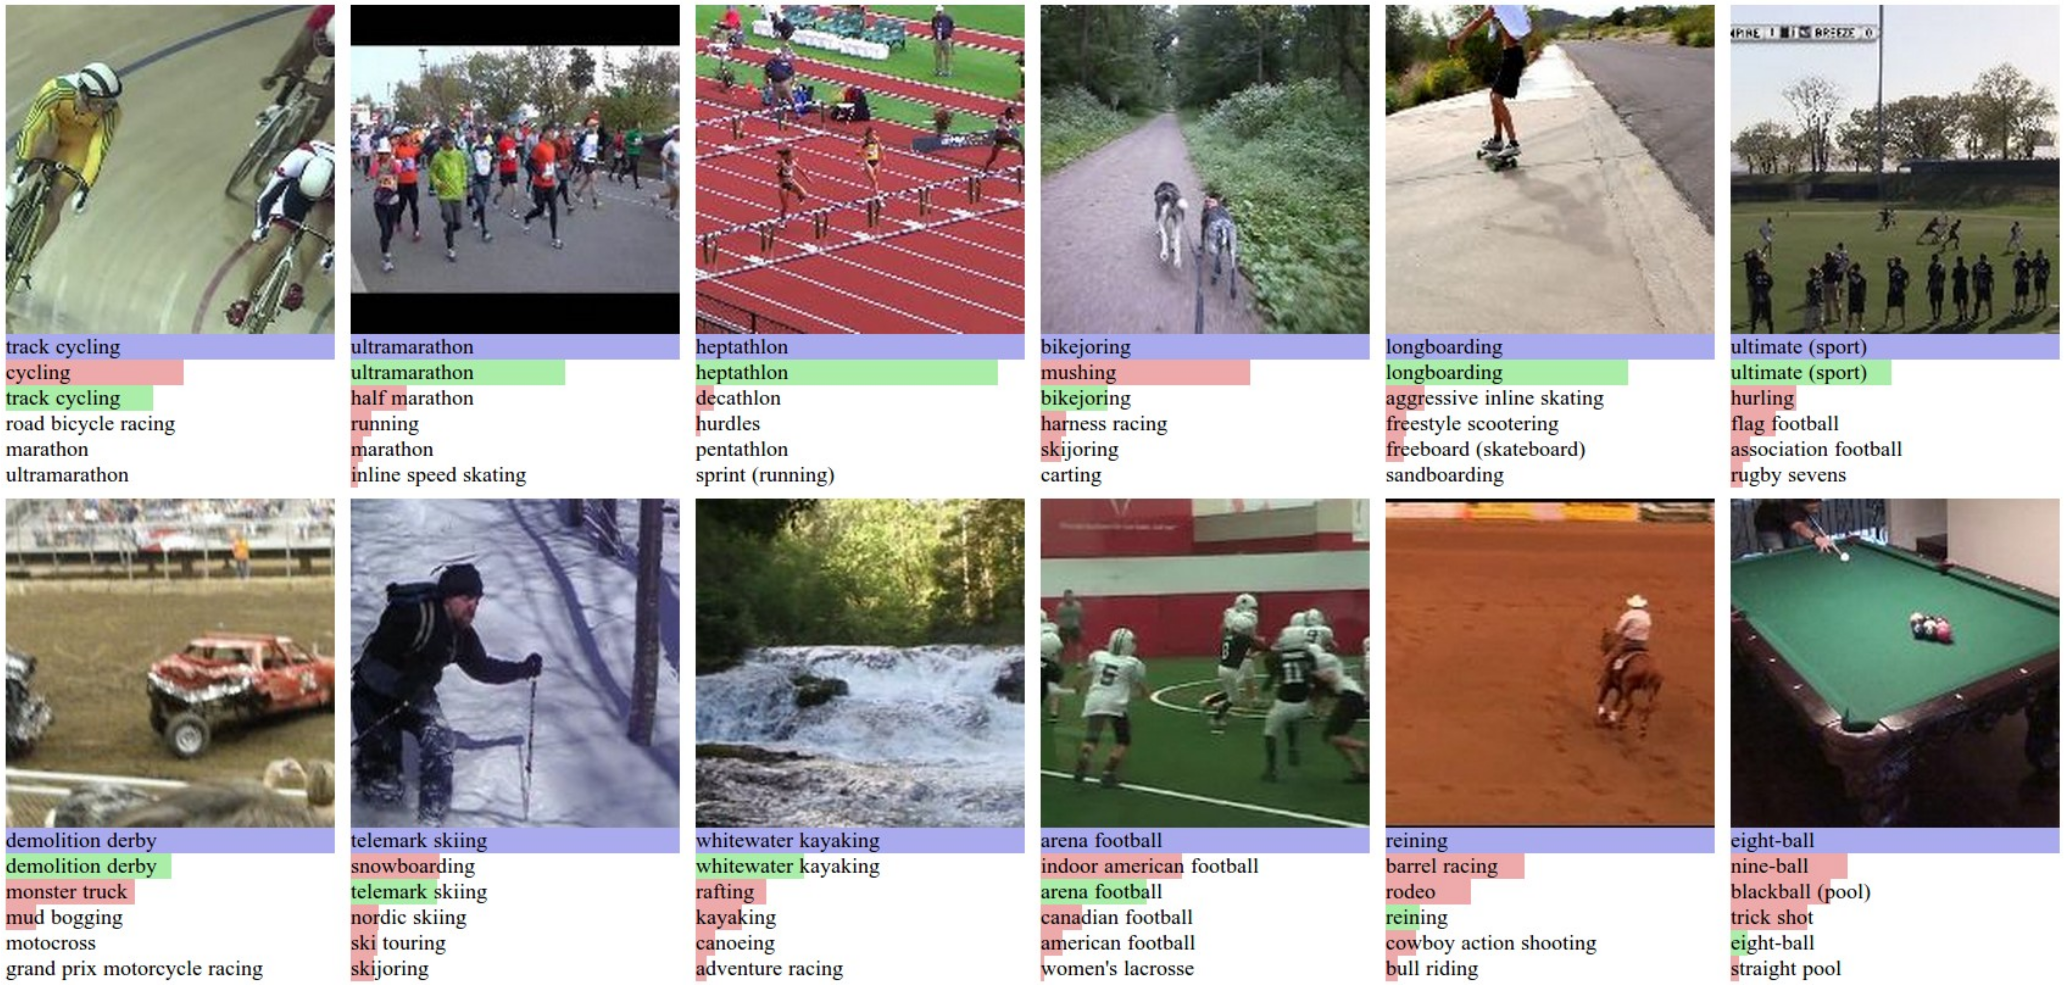
\includegraphics[width=\textwidth]{img_deep/largescale_classification}
    \caption{Classification of videos in the Sports-1M dataset. Blue label is the ground truth, below class predictions are shown with decreasing confidence. \cite{karpathy_large-scale_2014}}
    \label{fig:largescale_classification}
\end{figure}

In addition to comparing different fusion methods, the authors also implement a hand-crafted feature baseline approach, that extracts multiple kinds of hand-crafted local features from each video and aggregates them according to the bag-of-words paradigm.
The resulting feature histogram representations are classified into action classes using a multilayer neural network, with rectified linear activation units.

The performance of the studied approaches is shown in table \ref{tab:largescale_results}:
\begin{table}[H]
    \centering
    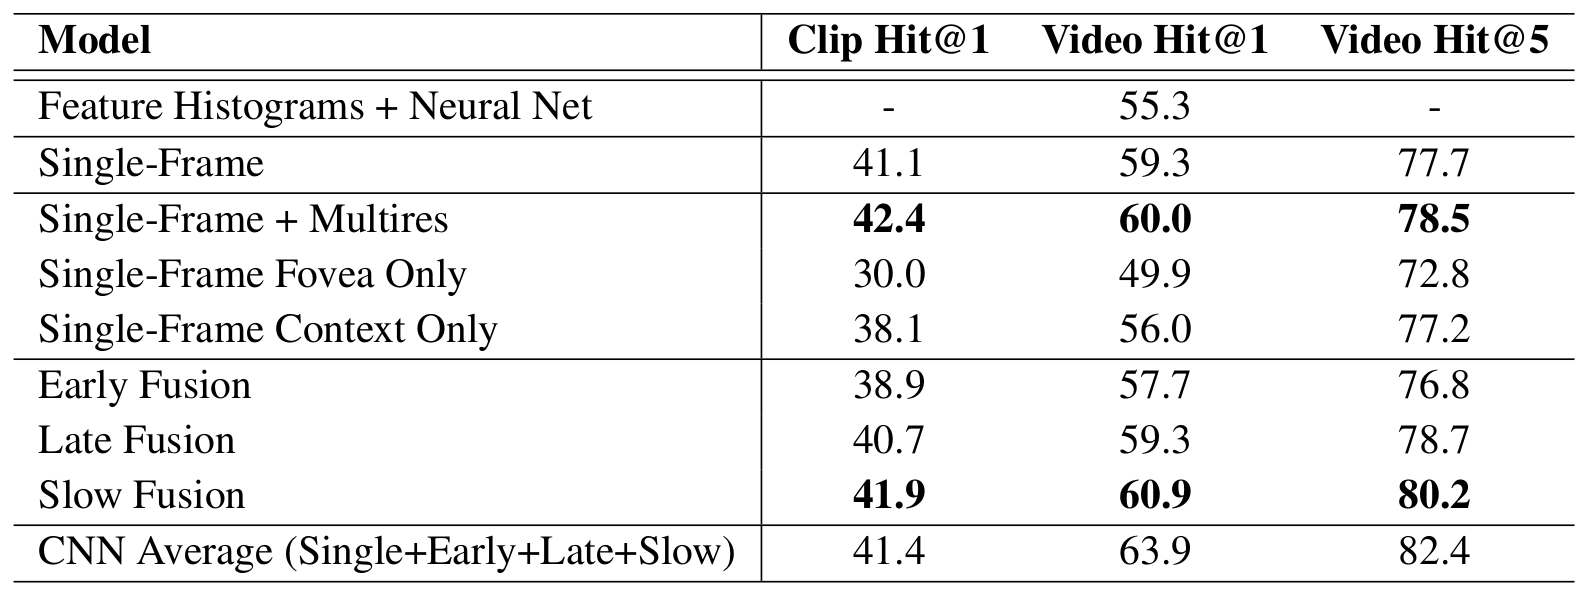
\includegraphics{img_deep/largescale_results}
    \caption{Results of different architectures on the Sports-1M dataset. Hit@$k$ denotes the percentage of test samples, that had at least one of their class labels included in the top $k$ predictions. \cite{karpathy_large-scale_2014}}
    \label{tab:largescale_results}
\end{table}

The results show, that the deep models (\textit{early}, \textit{late} and \textit{slow-fusion}) consistently outperform the hand-crafted feature baseline.
Compared to each other, the deep models perform similarly well, despite their different convolutional architectures.
The \textit{slow fusion} model, that uses 3D convolutions in all convolutional layers, outperforms the other fusion approaches by a small margin.
\textcite{karpathy_large-scale_2014} describe the performance difference of between fusion models as ``surprisingly insignificant''\cite{karpathy_large-scale_2014}.
The single-frame model performs noticably well on it's own.
The authors suspect, that the motion aware networks suffer from camera movements such as translations or zoom.

Since the training time of a network heavily influences the amount of evaluations that can be conducted using different hyperparameter settings, it is of great interest to reduce the training time for neural networks, which lies in the in the order of weeks for CNNs\cite{karpathy_large-scale_2014}, while maintaining accuracy.

The authors therefore propose a multiresolution architecture, that is shown in figure \ref{fig:largescale_multiresolution}.
\begin{figure}[H]
    \centering
    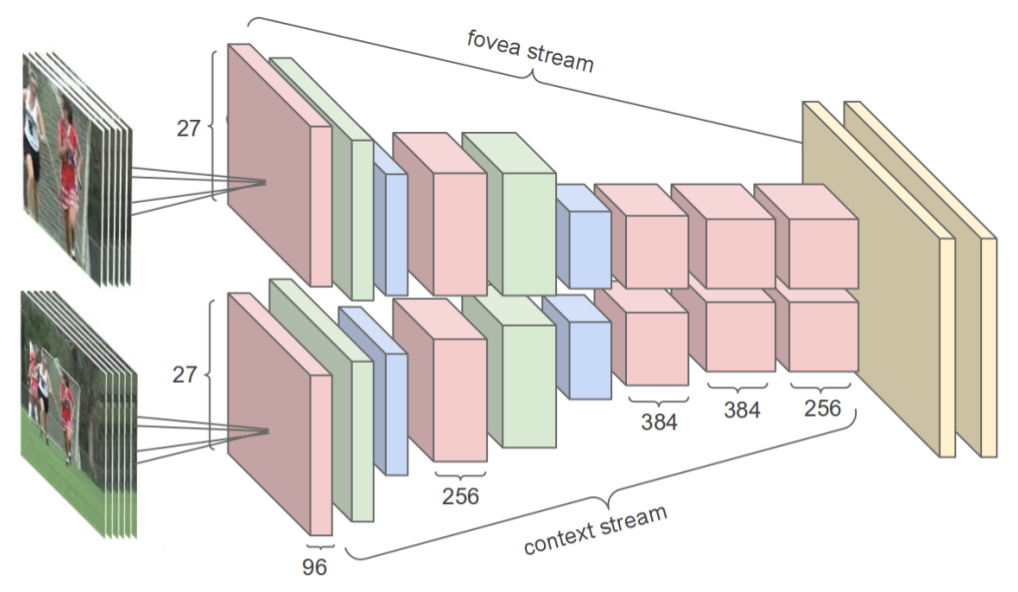
\includegraphics[width=0.75\textwidth]{img_deep/largescale_multiresolution.png}
    \caption{Multiresolution CNN architecture \cite{karpathy_large-scale_2014}}
    \label{fig:largescale_multiresolution}
\end{figure}

The multi-resolution network processes input videos with a resolution of $178\times178$ pixel.
The context stream receives a downsampled version of the input frames, which contain the complete field of view but have a decreased resolution of $89\times89$ pixel.
The fovea stream works on just the $89\times89$ pixel sized center of the original input frames.
Both streams are implemented as the same CNN architecture and the outputs of both streams are fed into two fully connected layers, where their information is merged and a class prediction is calculated.

The input dimensionality of the multiresolution architecture is decreased by a factor of $2$ compared to processing the raw $178\times178$ pixel input video in one stream.
The authors achieved a reduction in training time by a factor of 2-4, while maintaining the accuracy of the system (see table \ref{tab:largescale_results}).


\subsubsection{Learning Spatiotemporal Features with 3D Convolutional Networks (2015)}
\textcite{tran_learning_2015} create a generic spatio-temporal feature extractor, by training a very deep 3D ConvNet on the large-scale action recognition dataset Sports-1M \cite{karpathy_large-scale_2014}.
Given a human action video as input, the activations of the ConvNet's last fully connected layer form a descriptive feature vector, which represents the input.
The authors show, that the extracted feature representation, which they call \textit{C3D}, is generic enough to be reused on other vision tasks without requiring task-specific fine tuning of the model.
Merely a classifier (the authors use linear SVMs) has to be trained on the extracted \textit{C3D} features, given a video-based vision task.
The approach is evaluated for action recognition, action similarity labeling (ASLAN, see section \ref{chap:datasets} of this work), scene classification and object recognition.

Using a model based on 3D convolutions for \textit{C3D} is motivated by the recent review of fusion methods, published by \textcite{karpathy_large-scale_2014}, which showed that using 3D convolutions in all convolutional layers of a CNN performs best for action recognition (\textit{Slow Fustion}).  
The authors conclude that 3D convolutions preserve temporal information along the processing stages of a deep CNN, because they result in a 3 dimensional feature map.
In contrast 2D convolutions the temporal relations among frames after each convolutional layer by only processing frames spatially.
This is illustrated in following figure \ref{fig:c3d_2dconv3dconv}.
\begin{figure}[H]
    \centering
    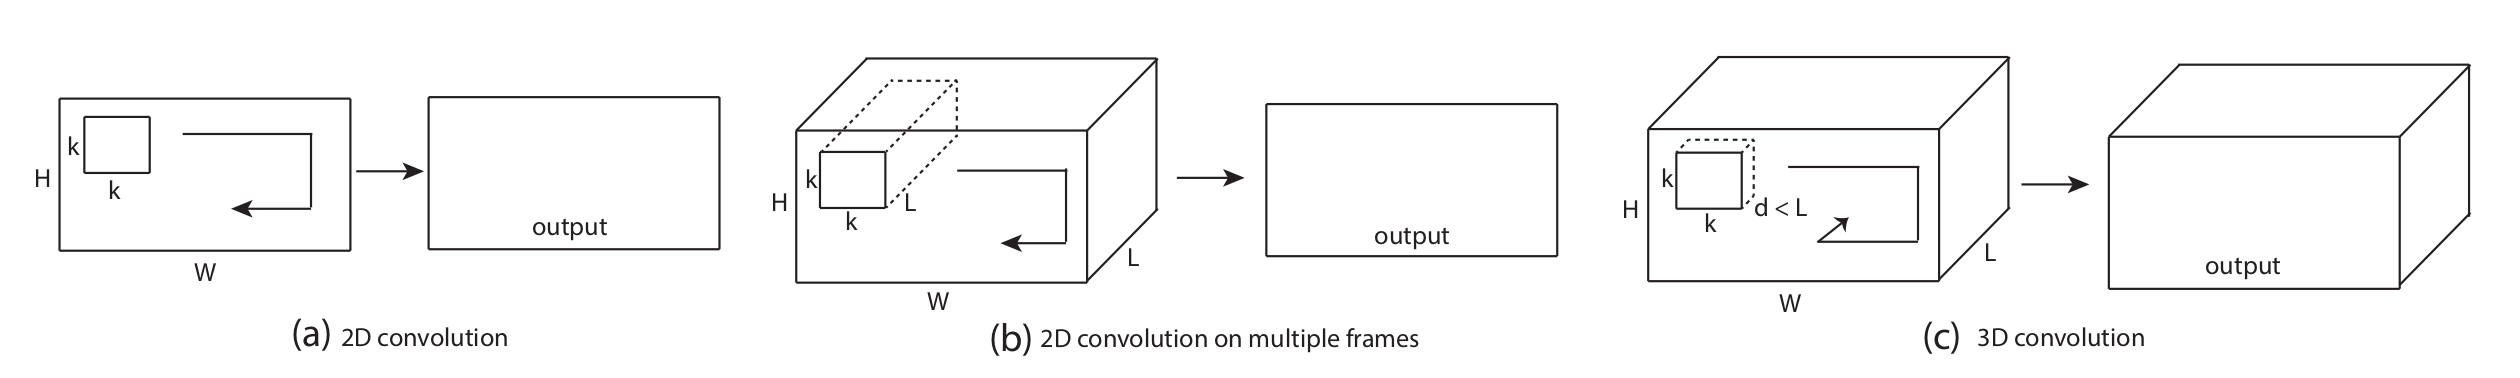
\includegraphics[width=\textwidth]{img_deep/c3d_2dconv3dconv}
\caption{Dimensionality of convolutions: a) 2D convolution on a single image results in a 2D feature map. b) 2D convolution on multiple frames, interpreted as different channels of the input, results in a 2D feature map because results of individual frames are summed. c) 3D convolution on multiple frames results in a 3D feature map, therefore preserving the temporal dimension \cite{karpathy_large-scale_2014}}
    \label{fig:c3d_2dconv3dconv}
\end{figure}

To find the best performing architecture, the authors first perform experiments on the medium-scale dataset UCF-101\cite{soomro_ucf101:_2012}, because using a large-scale dataset would be too time-consuming.
For these experiments, all trained networks take inputs of dimension $128\times171\times16$ (\textit{frame width} $\times$ \textit{frame height} $\times$ \textit{number of frames}, in three color channels each).
More specifically, the network architecture is designed as follows:
\begin{itemize}
    \item 5 convolutional layers with 64, 128, 256, 256 and 256 filters respectively.
    \item Each convolutional layer is followed by a max-pooling layer with filter size $2\times2\times2$ (except for the first layer, which has a filter size of $1\times2\times2$ for not collapsing the temporal information too early).
    \item Two fully connected layers with 2048 neuraons each at the end and an additional softmax layer with one output per action class for training.
\end{itemize}

The work of \textcite{simonyan_very_2014}, regarding 2D convolutional neural networks, suggests that $3\times3$ convolutional kernels yield best results in deep architectures .
The authors therefore fix the spatial kernel size in their 3D convolutions to $3\times3$ and vary the temporal depth of the kernel $d$.
For finding the best parameter, the depth $d$ is varied according to the following two methods, results are shown in figure \ref{fig:c3d_temporaldeptheval}:
\begin{enumerate}
    \item Homogeneous temporal depth: The kernels across all convolutional layers have the same temporal depth. Four networks are evaluated with $d \in \{1, 3, 5, 7\}$.
    \item Varying temporal depth: The temporal depth changes across the convolutional layers. Two schemes are being evaluated. Increasing temproal depth $3-3-5-5-7$ and decreasing temporal depth $7-5-5-3-3$.
\end{enumerate}

\begin{figure}[H]
    \centering
    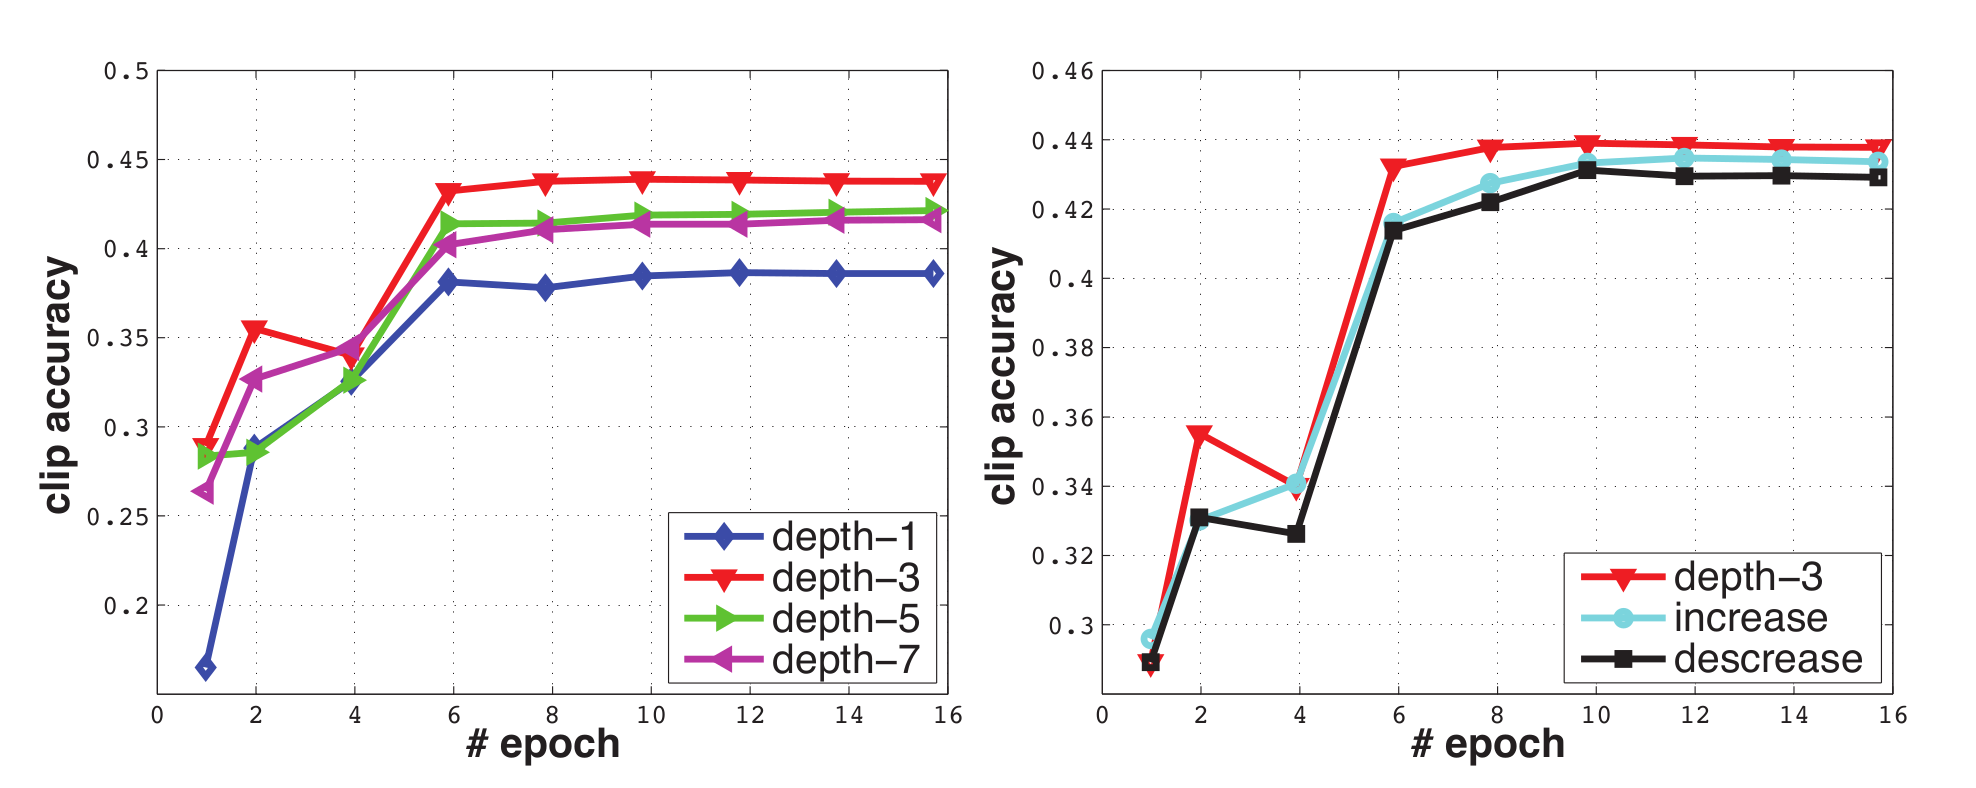
\includegraphics[width=\textwidth]{img_deep/c3d_temporaldeptheval}
    \caption{Clip accuracy for different temporal kernel depths over training epochs on UCF101. Left shows homogeneous temporal depth, right shows varying temporal depth. \cite{tran_learning_2015}}
    \label{fig:c3d_temporaldeptheval}
\end{figure}

The results indicate, that a fixed temporal depth of 3 performs best among all tested settings.
Testing a spatial kernel resolution of $5\times5$ with the same variations for $d$ yielded the same result.
The authors therefore conclude that $3\times3\times3$ kernels are the best choice in 3D convolutional networks.

Using this result, the authors design the architecture for extracting C3D features with 3x3x3 convolutional kernels as follows: 8 convolutional layers, 5 pooling layers, two fully connected layers and a softmax output layer as can be seen in figure \ref{fig:c3d_architecture}.

\begin{figure}[H]
    \centering
    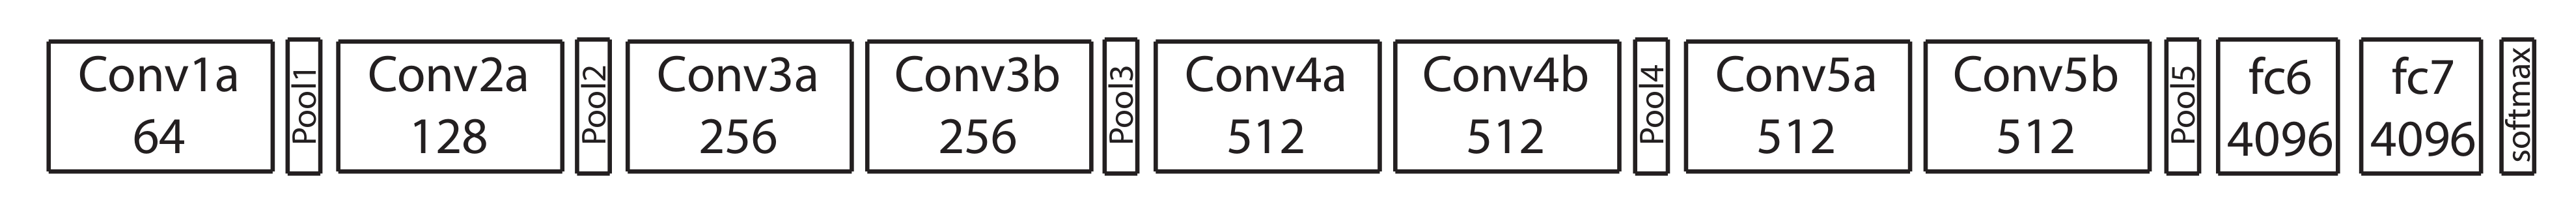
\includegraphics[width=\textwidth]{img_deep/c3d_architecture}
    \caption{C3D architecture. Number of filters is given in each box. \cite{tran_learning_2015}}
    \label{fig:c3d_architecture}
\end{figure}

\textbf{Training} \\
The network is trained on the large-scale dataset Sports-1M to learn spatio-temporal features.

Five two second long clips are extracted from every training video and resized to the input dimensions of 128x171 pixel.

The training inputs are randomly extracted video volumes from these clips of size 112x112x16 (using temporal and spatial jittering).

Training is conducted with stochastic gradient descent with batch size of 30.

\textbf{Testing} \\
A single center crop of a testing-video is passed through the network to obtain a clip-preditction.

For obtaining video-predictions, the predictions for 10 clips which were extracted randomly from the test-video are being averaged.

The network trained from scratch yields top-5 accuracy at action recognition on the Sports-1M dataset of $84.4\%$. The authors also try to boost the performance by pre-training the model on an internal dataset (called I380K), which results in a top-5 accuracy of $85.5\%$.

The authors propose a standardized method to extract C3D features using their model and evaluate them on several video analysis tasks:
\begin{enumerate}
    \item Action recognition on UCF-101 dataset: \\
    A single C3D net obtains an accuracy of 82.3\%.
    Three networks combined obtain 85.2\%.
    In order to outperform the results of \textcite{simonyan_two-stream_2014} or \textcite{ng_beyond_2015}, C3D has to be combined with the improved dense trajecotries approach \cite{wang_action_2013}, which results in an accuracy of 90.4\%.

    \item Action Similarity Labeling (ASLAN \cite{kliper-gross_action_2012}): \\
    C3D features classified with a linear SVM outperforms the state-of-the-art method \cite{peng_large_2014} by 9.6\%.

    \item Scene Recognition on YUPENN and Maryland benchmark: \\
    Using C3D features outperforms the state-of-the-art method on both benchmarks \cite{feichtenhofer_bags_2014}.

    \item Object Recognition on the Egocentric datset \cite{ren_egocentric_2009}: \\
    C3D features outperfrom the method of \cite{ren_egocentric_2009} but perform worse than an ImageNet baseline.
\end{enumerate}

Additionally to good results on various video analysis datasets, the authors note several advantages of using their features:
\begin{enumerate}
    \item They are simple to compute by making the pre-trained 3D CNN model available
    \item The features are compact and discriminative, which makes them scalable to large-scale analysis tasks.
    \item They are efficient to compute, because of the fast forward processing in neural networks.
\end{enumerate}


\subsubsection{Long-term Temporal Convolutions for Action Recognition -- Varol et al. (2016)}
%Extensions of CNNs to action recognition in video have been proposed in several
%recent works [6, 12, 13]. Such methods, however, currently show only moderate
%improvements over earlier methods using hand-crafted video features [5].

\textcite{varol_long-term_2016} address, similar to \textcite{baccouche_sequential_2011}, the common drawback of recent CNN extensions in action recognition, that class labels are learned from very short video subsequences only, i.e.\ a temporal extend of only 1-16 input frames can be processed by the architectures at a time.\cite{ji_3d_2013}\cite{karpathy_large-scale_2014}\cite{tran_learning_2015}

Instead of using a recurrent neural network for classifying convolutionally extracted spatio-temporal features, which takes the temporal evolution of features into account (as done by \textcite{baccouche_sequential_2011}), in this publication the authors study the effects of increasing the number of input frames of a 3D convolutional architecture on the performance in action recognition.

The authors call their approach long-term temporal convolutions. Their contribution in this work is two-fold:
\begin{enumerate}
    \item Systematical evaluation of the influence of the temporal extend, i.e.\ the number of input frames $T = \{20, 40, 60, 80, 100\}$, on the performance of a 3D CNN architectures for video action recognition.  
    \item Confirming the importance of high-quality optical flow inputs, in order to learn accurate video features with a 3D CNN architecture for human action recognition.
\end{enumerate}

Processing an increased temporal extend has to be compensated with a decreased spatial resolution, in order to not exceed computational limitations.
The studied architectures therefore process spatial resolutions of 58x58 or 71x71 pixels.

The authors' 3D CNN architecture is shown in figure \ref{fig:longterm_architecture}.

\begin{figure}[H]
    \centering
    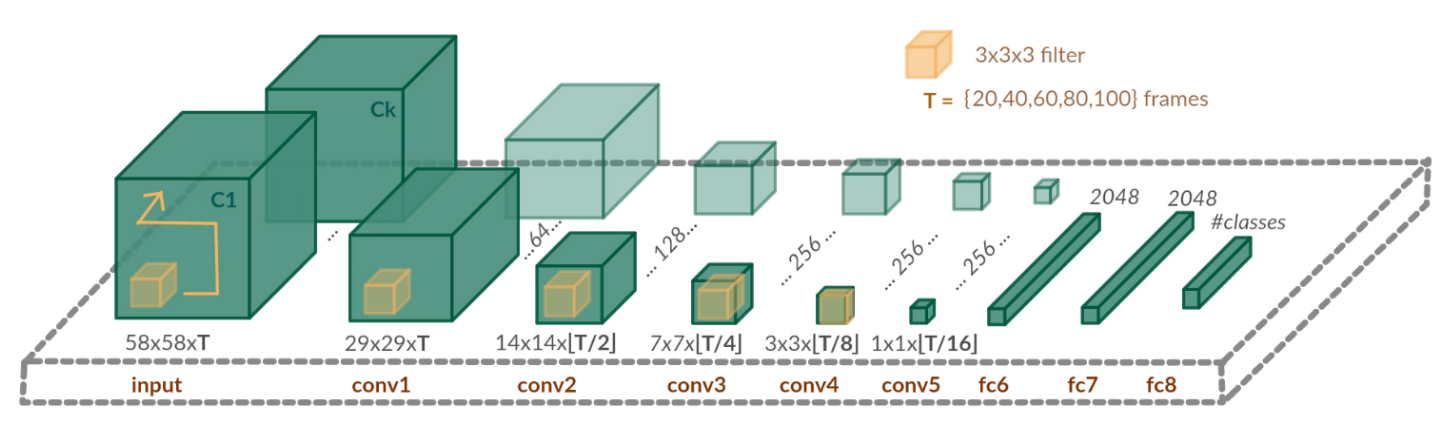
\includegraphics[width=\textwidth]{img_deep/longterm_architecture}
    \caption{3D CNN architecture for evaluating the influence of temporal extend on action recognition performance. \cite{varol_long-term_2016}}
    \label{fig:longterm_architecture}
\end{figure}

Architectural details:

\begin{itemize}
    \item 5 space-time convolutional layers with 64, 128, 256, 256 and 256 feature maps (also called 3D convolutions).
    \item 3x3x3 space-time convolutional kernels in every convolutional layer.
    \item After each convolutional layer: One layer of rectified linear units (ReLU) and one layer of max-pooling with filter size 2x2x2 except in the first layer where it is 2x2x1.
    \item 3 fully connected layers as classifier with sizes 2048, 2048 and number of classes.
        The fully connected layers also use rectified linear units as activation functions and a softmax layer at the end of the network.
\end{itemize}

As a baseline approach the authors first implement their architecture with inputs of size 112x112x16, beacause it can be directly compared to the work of \textcite{tran_learning_2015}.
The authors initially study the performance between the 16 frame baseline and a 60 frame network, which takes inputs of size 58x58x60 (spatial size has to be decreased to remain computationally tractable).

In order to then systematically investigate the influence of temporal extend on the action recognition performance, the authors implement their architecture with different numbers of input frames $T = \{20, 40, 60, 80, 100\}$ and different spatial resolutions ${58 \times 58, 71 \times 71}$.

Additionally the influence of using optical flow inputs on the performance, specifically the influence of different sources of optical flow, is evaluated. These namely are:
\begin{enumerate}
    \item MPEG flow, which directly can be obtained from the video encoding. It is a fast alternative to regular optical flow estimators, but has low spatial resolution and is not available for all video frames.
    \item Farneback optical flow estimator cite ??, which is fast, but calculates noisy flow fields.
    \item Brox optical flow estimator cite ??, which generates highest quality optical fields but is slower than the other two methods.
\end{enumerate}

Example flow estimations for all three methods are shown in figure \ref{fig:longterm_optflow}.

\begin{figure}[H]
    \centering
    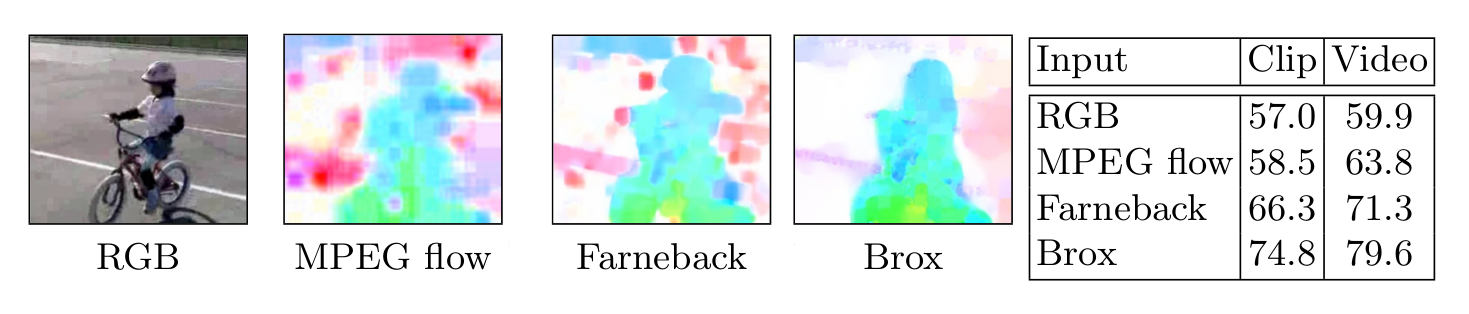
\includegraphics[width=\textwidth]{img_deep/longterm_optflow}
    \caption{Add caption here}
    \label{fig:longterm_optflow}
\end{figure}

The networks are trained on the UCF-101 and HMDB-51 dataset using stochastic gradient descent with negative log-likelihood criterion.

The authors generate training inputs by randomly sampling video subsequences with the desired spatial and temporal dimensions from the input videos, which in general have a higher resolution and are temporally longer than needed. The authors call this form of pre-processing \textit{random clipping}.

An alternative method for creating suitable network inputs during training is called \textit{multiscale cropping}.
Smaller input volumes than needed are cropped from the training videos and then rescaled to fit to the input dimensions of the network.
The size of the crop is determined by rendomly selected factors for frame width and height from $\{1.0, 0.875, 0.75, 0.66\}$.
Finally the input is flipped with a probability of 50\%.

Dropout is used during training independent of the selected cropping method.

Details of the testing-procedure are:
\begin{enumerate}
    \item The video under test is divided into sequences of length $T$ with temporal stride 4, each called a clip.
    \item For each video clip, 10 crops are being classified: The 4 corners, the center and their horizontal flips.
    \item The overall video classification is obtained by averaging over crop scores and clip scores.  
\end{enumerate}

Two evaluation metrics are used to compare the networks: 
\begin{enumerate}
    \item Clip-accuracy: Each clip is assigned the class according to the highest softmax-score and the number of correctly classified clips is measured.
    \item Video-accuracy (i.e. the standard evaluation protocol): The per-clip softmax scores are averaged and the maximum value defines the class label for the video. The authors report their final resutlts by taking the mean over the results on the three test splits of the datasets.
\end{enumerate}

\textbf{Optical flow results:} \\
The influence of optical flow quality on the action recognition performance is depicted in the table on the right of figure \ref{fig:longterm_optflow}.

For this evaluation a network with 60 input-frames was trained on UCF-101 split 1 from scratch.

The authors find, that high quality optical flow, i.e.\ Brox flow, can boost the action recognition performance by nearly 20\%.

Even using low-quality MPEG-flow outperforms regular RGB inputs.

The authors therefore conclude, that using high-quality optical flow inputs is critical for learning competitive human action features from video.

\textbf{Data-augmentation and dropout results:} \\
Results for the used data augmentation methods \textit{Random Clipping}, \textit{Multiscale Cropping} and \textit{Dropout} are shown below in table \ref{tab:longterm_preprocessing}.
Best performance is obtained when combining all three methods.

\begin{table}[H]
    \centering
    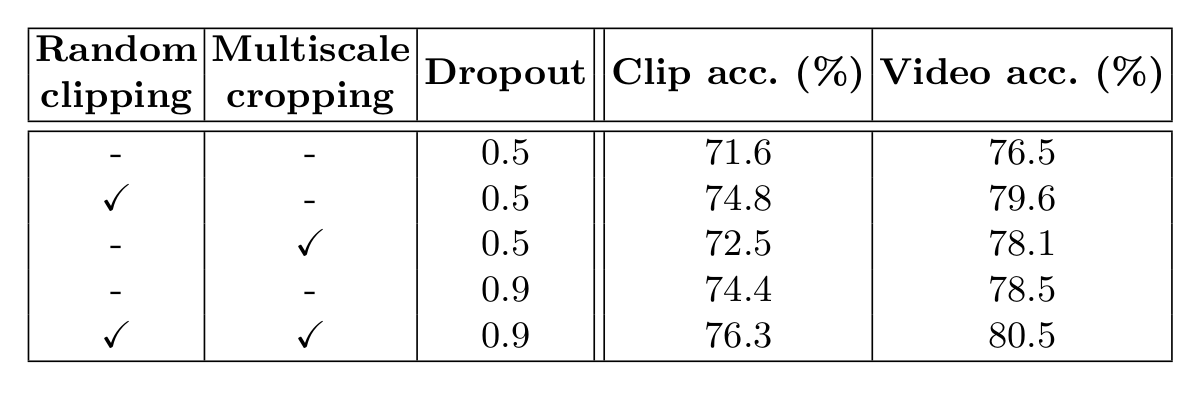
\includegraphics[width=0.75\textwidth]{img_deep/longterm_preprocessing}
    \caption{Evaluation of data-augmentation methods and dropout on a 60 input-frame network, trained on UCF-101 (split 1) from scratch using Brox flow as input modality \cite{varol_long-term_2016}}
    \label{tab:longterm_preprocessing}
\end{table}

\textbf{Comparison 16 frame against 60 frame input:}\\
The 16 frame network is equivalent to the C3D architecture in \cite{tran_learning_2015} and therefore enables direct comparison to the long-term temporal convolution approach of this work (the 60 frame network).

The evaluation results on the UCF-101 dataset (split 1) for RGB and optical flow inputs as well as different data augmentations and dropout are shown in table \ref{tab:longterm_16vs60} below.

\begin{table}[H]
    \centering
    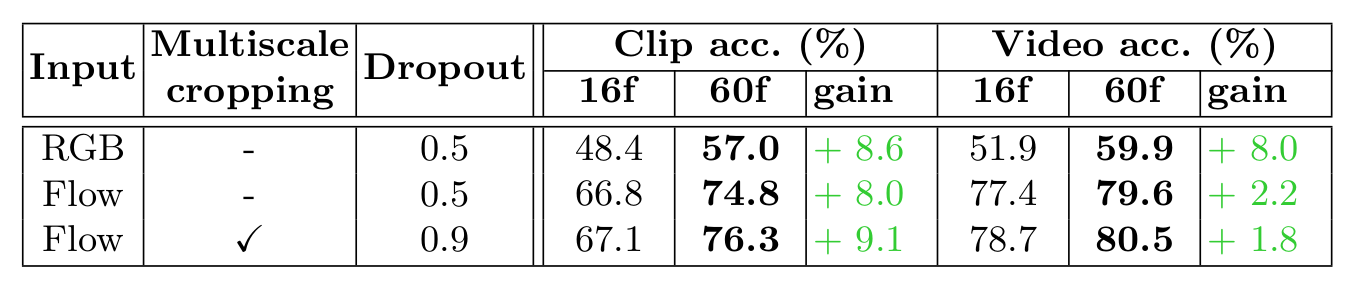
\includegraphics[width=\textwidth]{img_deep/longterm_16vs60}
    \caption{Performance for 16 frame against 60 frame inputs, evaluated on UCF-101 (split 1) \cite{varol_long-term_2016}}
    \label{tab:longterm_16vs60}
\end{table}

The results show that long-term temporal convolutions in the 60 frame network persistently outperform the 16 frame counterpart.

The authors note, that the complexity of the networks, i.e.\ the number of trainable parameters, is similar.

Results for the clip accuracy are more prominent, because video evaluation already averages and aggregates the available information over the whole video.

The authors repeat the comparison on the HMDB-51 (split 1) dataset and additionally evaluate the effects of pre-training the networks on the UCF-101 dataset, because HMDB-51 is significantly smaller than UCF-101.

Results are shown in table \ref{tab:longterm_pretraining} below.

\begin{table}[H]
    \centering
    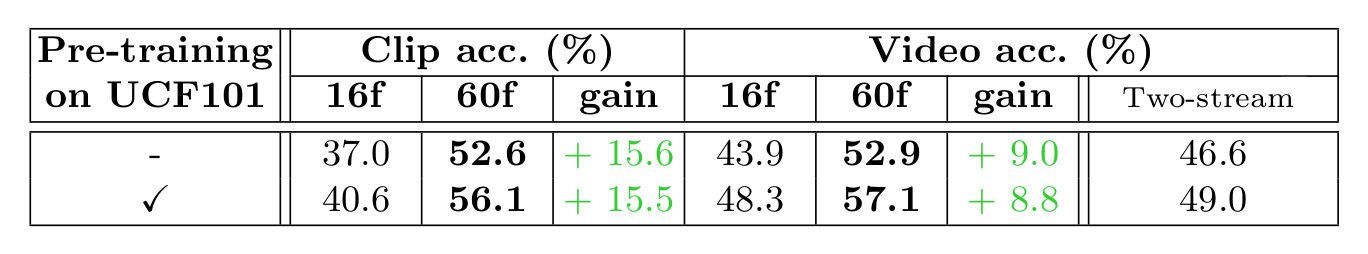
\includegraphics[width=\textwidth]{img_deep/longterm_pretraining}
    \caption{Performance for 16 frame against 60 frame inputs, evaluated on HMDB-51 (split 1). Flow input, random clipping, multiscale cropping and 0.9 dropout are used. \cite{varol_long-term_2016}}
    \label{tab:longterm_pretraining}
\end{table}

The results again indicate, that using long-term temporal convolutions leads to significant increase in action recognition accuracy.

Pre-training the networks yields significant improvement over training it from scratch. 

\begin{figure}[H]
    \centering
    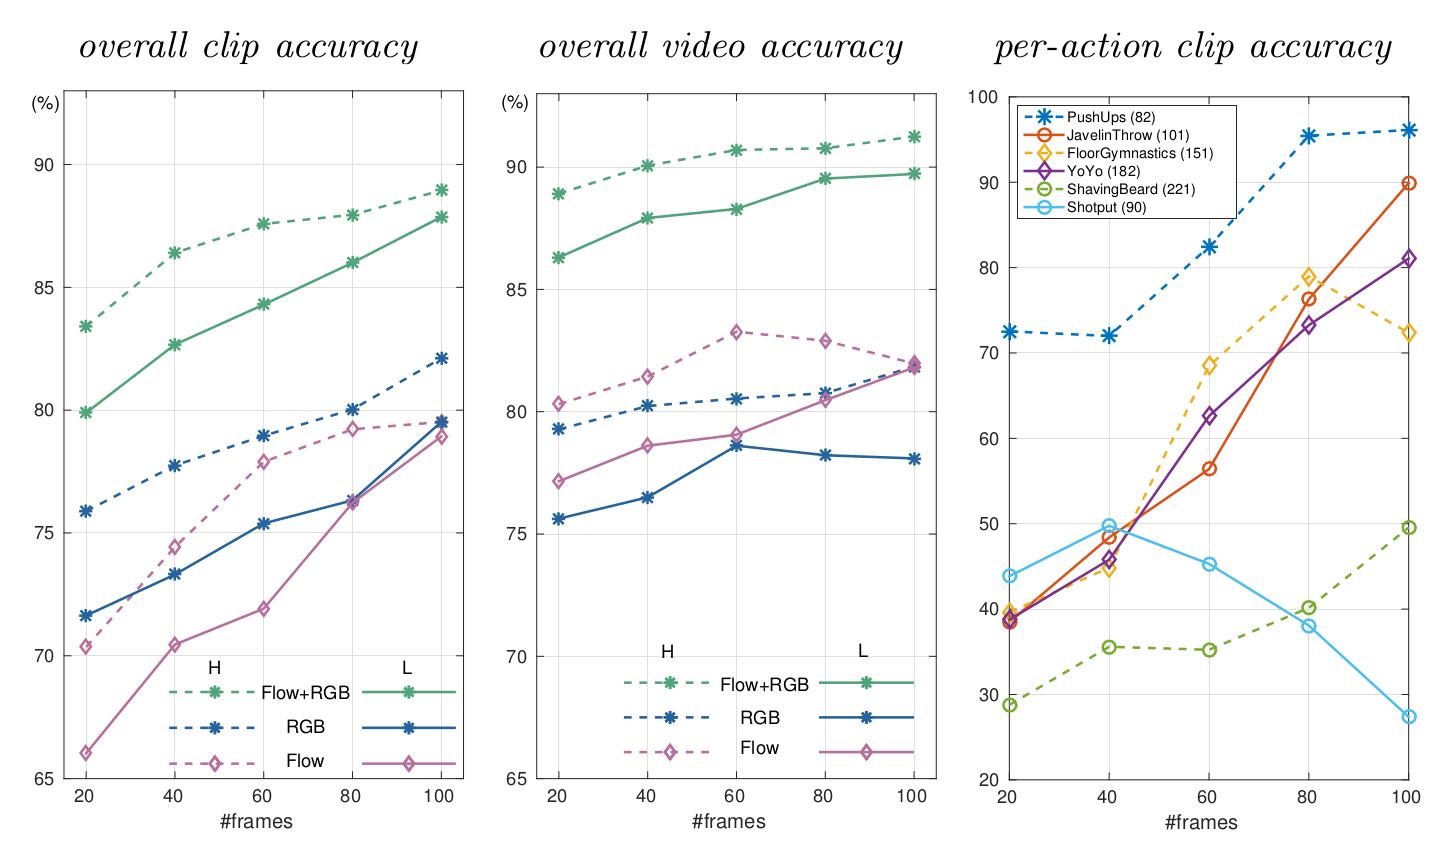
\includegraphics[width=\textwidth]{img_deep/longterm_systematical}
    \caption{<+caption text+>}
    \label{fig:<+label+>}
\end{figure}

\subsubsection{Summary and Comparison}
Most of the current CNN methods use architectures with 2D convolutions, enabling shift-invariant representations in the image plane. Meanwhile, the invariance to translations in time is also important for action recognition since the beginning and the end of actions is unknown in general. Laptev 2016
Note: No need for action detection???

%---------------------------------------------------------------------------------------------------------------------------------------------------------------------------------------
\newpage
\subsection{Multiple Stream Networks}
The most successfull architecture at action recognition. They are equally powerful as the improved dense trajectories approach. cite TDD ??

These approaches use the decomposability of videos into a spatial component (analysing different frames) and a temporal component (analysing the change between frames) for action recognition.

Underlying principle: Temporal dimension has different characteristics than the spatial dimension and should therefore be handled separately, not in a joint 3D space.

The first architecture of this kind was proposed in 2014 by Simonyan and Zisserman.


\subsubsection{Two-Stream Convolutional Networks for Action Recognition in Videos - Simonyan and Zisserman (2014)}

The authors propose a novel architecture for action recognition with two separate recognition streams (spatial- and temporal-stream) which are combined by late fusion.

The authors evaluate two different fusion methods: building the average of both network's outputs and training a linear multi-class SVM on stacked $L_2$-normalised softmax scores.

This approach is motivated by the two-streams hypothesis cite (??), according to which the human visual cortex contains two paths: the ventral stream for object recognition and the dorsal stream for recognising motion.

Both streams are implemented as deep CNNs, with the rectification activation function for all hidden units.

\begin{figure}[H]
    \centering
    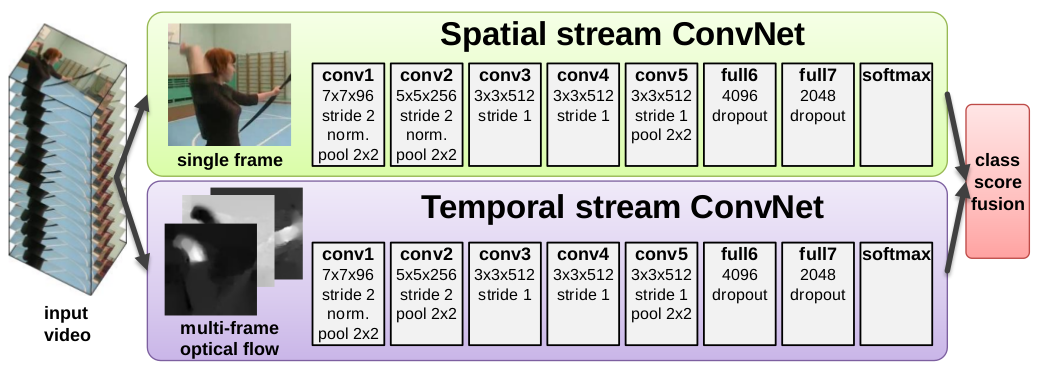
\includegraphics[width=0.9\textwidth]{img_deep/twostream_architecture}
    \caption{Two-stream architecture for video classification, depicting the spatial- and temporal-stream with implementation details as deep Convolutional Neural Network \cite{simonyan_two-stream_2014}}
    \label{fig:twostream_architecture}
\end{figure}

Spatial stream: Takes single video frames as input. Performs action recognition from still images and is fairly competitive on its own. Basically an image recognition architecture. Advantage: Can be pre-trained using large amount of image data, here from the ImageNet challenge dataset cite (??).

Spatial part of a video, i.e. the individual static frames, convey information about the objects and persons in the scene.

Temporal stream: is trained to recognize actions from motions given in the form of dense optical flow.

The temporal part of a video, i.e. the change between frames, conveys information about the movement of the observer (camera) and the movement of objects in the scene.

The second normalisation layer was removed from the the temporal stream network in order to reduce memory usage.

The authors propose two methods for constructing the input to the temporal network by stacking optical flow displacement fields along several consecutive frames of the input video.

\textbf{Optical Flow Stacking:} \\
A dense optical flow field $\mathbf{d}_t(u,v)$ of two consecutive frames at times $t$ and $t+1$ can be thought of as a two dimensional vector-field, which maps the displacement of each pixel along the transition from frame $t$ to $t+1$. In this case $u,v \in \mathbb{N}$, $1 \leq u \leq w$ and $1 \leq v \leq h$ where $w$ and $h$ are the width and height of the video frames.

The horizontal and vertical components $d_t^x(u,v)$, $d_t^y(u,v)$ can be interpreted as image channels.

This method constructs the input volume $I_\tau \in \mathbb{R}^{w \times h \times 2L}$ of the temporal stream network by stacking the horizontal and vertical components of the dense optical flow field along $L$ consecutive frames, beginning at time $\tau$. Formally, with $1 \leq k \leq L$:
\begin{align*}
    I_\tau(u,v,2k-1) = d_{\tau + k - 1}^x(u,v) \\
    I_\tau(u,v,2k) = d_{\tau + k - 1}^{y}(u,v)
\end{align*}

\textbf{Trajectory Stacking:} \\
Instead of sampling at fixed locations in each frame, this methods samples the dense optical flow field along the motion trajectories of the initial points in frame $\tau$.

Let $\mathbf{p}_k$ denote the motion trajectory of initial point $(u,v)$. With $1 < k \leq L$ and \mbox{$\mathbf{p}_1 = (u,v)$} the trajectory is recursively defined by:
\begin{align*}
    \mathbf{p}_k = \mathbf{p}_{k-1} + \mathbf{d}_{\tau + k - 2}(\mathbf{p}_{k-1})
\end{align*}

The input volume can then be constructed by sampling the horizontal and vertical optical flow components along these trajectories.

\begin{align*}
    I_\tau(u,v,2k-1) = d_{\tau + k - 1}^x(\mathbf{p}_{k}) \\
    I_\tau(u,v,2k) = d_{\tau + k - 1}^y(\mathbf{p}_{k})
\end{align*}

\begin{figure}[H]
    \centering
    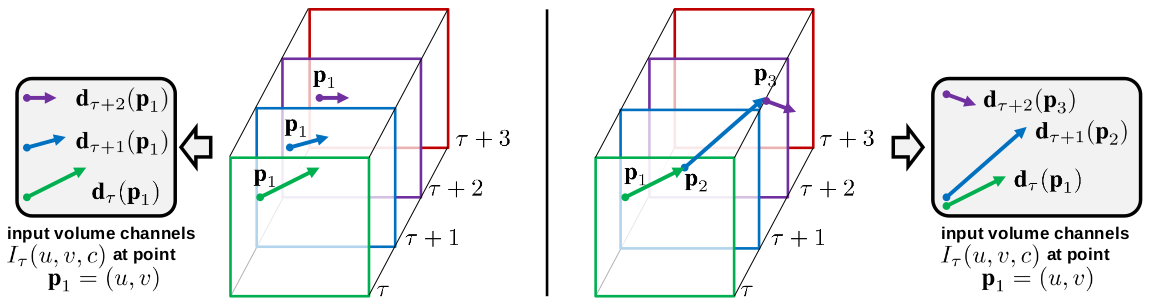
\includegraphics[width=0.9\textwidth]{img_deep/trajectory_stacking}
    \caption{Construction of input volumes from multi-frame optical flow. Left: Optical Flow Stacking. Right: Trajectory Stacking \cite{simonyan_two-stream_2014}}
    \label{fig:trajectory_stacking}
\end{figure}

Since the Convolutional Networks require fixed sized inputs, the authors sample a $224 \times 224 \times 2L$ subvolume from $I_\tau \in \mathbb{R}^{w \times h \times 2L}$ and use it as the temporal networks input.

By using optical flow, the authors explicitly incorporate a representation of motion in their action recognition architecture.

The authors further describe two optional techniques that are evaluated for constructing the inputs with either one of optical flow stacking methods.
\begin{enumerate}
    \item \textbf{Bi-directional Optical Flow}: The input volume $I_{\tau}$ is created by using regular forward optical flow from frame $\tau$ to $\tau + L/2$ and additionally calculated optical flow from frame $\tau$ to $\tau - L/2$ in the backwards direction. Stacking the horizontal and vertical components of these optical flow fields results in an input volume of length $L/2$ around frame $\tau$ in both directions. 
    \item \textbf{Mean flow subtraction}: The displacement vectors between two frames can dominantly be caused by global movement of the camera. Compared to regular camera-motion compensation, the authors use a simpler approach and just subtract the mean vector from each displacement field $\mathbf{d}_t$.
\end{enumerate}

An advantage of separating the spatial and the temporal stream is the possibility of pre-training the spatial net with large pre-existing image datasets (here ImageNet ILSVRC-2012 ??).

For training the temporal stream network with video-data, the authors address the general problem of video action recognition, that the existing datasets are too small in comparison to their image-dataset counterparts.

The authors use, according to the multi-task learning paradigm \cite{collobert_unified_2008}, the UCF-101 and the HMDB-51 dataset simultaneously for training the temporal stream network (see chapter ??). 

By training a network on several tasks (here UCF-101 classification and HMDB-51 classification), the network learns more general video representations, since the second task acts as regulariser and more data can be utilized.

The authors implement this by using two softmax classification layers, one for each dataset. Each softmax layer has its own loss function and the sum of the individual losses is taken as the overall training loss for computing the weight updates by backpropagation.

Training for both networks is conducted with mini-batch gradient descent with 256 randomly selected videos at each iteration. From each of those videos, a single frame is randomly chosen, a $224 \times 224$ sub-image is randomly cropped, randomly horizontal flipped, RGB jittered and then used as training input for the spatial stream network.

An optical flow volume is constructed for this selected frame as described above. For optical flow computation the authors use a fast implementation (0.06s per pair of frames) from the OpenCV toolbox. Despite it's speed, on-the-fly computation of optical-flow would be a bottleneck and is therefore pre-computed and stored for the complete datasets.

The creators of UCF-101 and HMDB-51 provide three splits of their datasets into training- and testing-data. The standard evaluation procedure is to report the average accuracy over those three splits, which the authors follow in this work as well.

The authors build their final design of the two-stream architecture by evaluating different setups for the spatial and temporal stream network on their own using UCF-101 (split 1).

Besides using two different dropout rate (0.5 and 0.9), the performance of the spatial-stream network is evaluated for:
\begin{enumerate}
    \item Training the complete network from scratch on UCF-101.
    \item Pre-training the network on ILSVRC-2012 and fine-tuning it on UCF-101.
    \item Pre-training the network on ILSVRC-2012 and fine-tuning of only the last (classification) layer.
\end{enumerate}

For evaluating the temporal-stream network a fixed dropout rate of 0.9 is chosen, because the network needs to be trained from scratch. The performance is then measured for:
\begin{enumerate}
    \item Using one or several (stacked) optical flow displacement fields $L \in {1,5,10}$.
    \item Regular optical flow stacking
    \item Trajectory stacking
    \item Using bi-directional optical flow
    \item Using mean subtraction
\end{enumerate}

The findings are presented in table \ref{tab:twostream_archeval}.

Spatial-stream network: The authors decided on pre-trained the network on ILSVRC and fine-tuning only the last layer.

Temporal-stream network: Mean subtraction and stacking multiple optical flows is beneficial, so $L=10$ is used as the default setting. Regular optical flow stacking performs better than trajectory stacking and bi-directional optical flow only yields slight improvement against forward optical flow. Therefore regular forwars optical flow stacking is chosen for the temporal-stream network.

The authors highlight that the temporal-stream network significantly outperforms the spatial-stream network, which confirms the importance of motion information for action recognition from video.

\begin{table}[H]
    \centering
    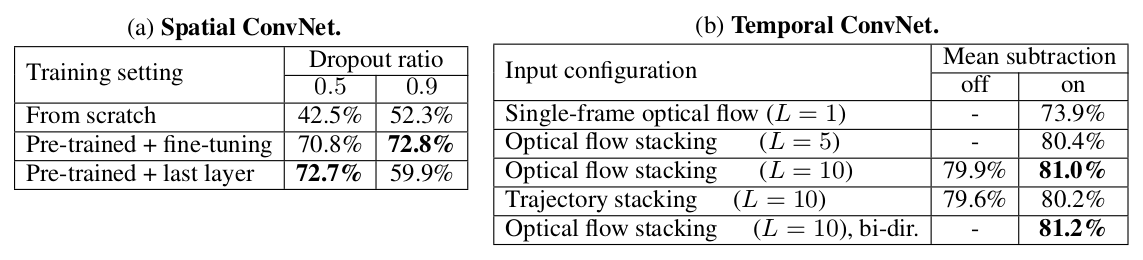
\includegraphics[width=\textwidth]{img_deep/twostream_archeval}
    \caption{Performance of the individual convolutional networks on UCF-101 (split 1) \cite{simonyan_two-stream_2014}}
    \label{tab:twostream_archeval}
\end{table}

After having found the optimal configurations for the individual temporal-stream and spatial-stream networks, the authors evaluate different fusion methods (averaging and SVM) and find that fusion by SVM performs best. The fused network's performance significantly improves over the individual network's performance, which implies, that the spatial and temporal recognition stream are complementary.

\begin{table}[H]
    \centering
    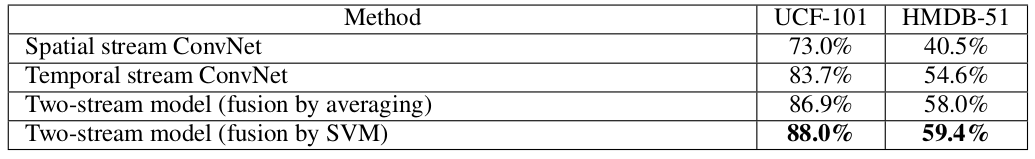
\includegraphics[width=\textwidth]{img_deep/twostream_results}
    \caption{Mean accuracy over three splits on UCF-101 and HMDB-51 \cite{simonyan_two-stream_2014}}
    \label{tab:twostream_results}
\end{table}

The results in table \ref{tab:twostream_results} show, that fusion by SVM works best.


\subsubsection{Beyond Short Snippets: Deep Networks for Video Classification -- Ng et al. (2015)}

\textcite{ng_beyond_2015} hypothesize that a global video description, i.e.\ a representation learned from the complete temporal evolution of a video, is important for accurate action recognition.

Similar to the approaches made in \cite{baccouche_sequential_2011} and \cite{varol_long-term_2016}, the goal of this work is to design and evaluate video processing architectures, that are able to incorporate video information over long time periods (tens of seconds), preferably over the complete video.

The authors discuss the results of \textcite{karpathy_large-scale_2014}, who discovered that spatio-temporal 3D convolutions applied on frame stacks of short video-subclips only yield marginally better performance than a single-frame baseline.

The following approach is therefore evaluated in this work (see also figure \ref{fig:beyondshort_overview}):
\begin{enumerate}
    \item 2D image features are obtained from still input frames by feeding them into a convolutional neural network (which incorporates 2D convolutions for processing still images).
    \item The resulting feature vectors for each frame, i.e.\ the activations of the last convolutional layers, are aggregated into a global video representation by using one of the following methods:
    \begin{itemize}
        \item A feature pooling architecture aggregates the CNN activations through several pooling layers, which are added after the last convolutional layer.
        \item A recurrent neural network uses layers of LSTM cells after the last convoultional layer to integrate frame information over time.
    \end{itemize}
\end{enumerate}

\begin{figure}[H]
    \centering
    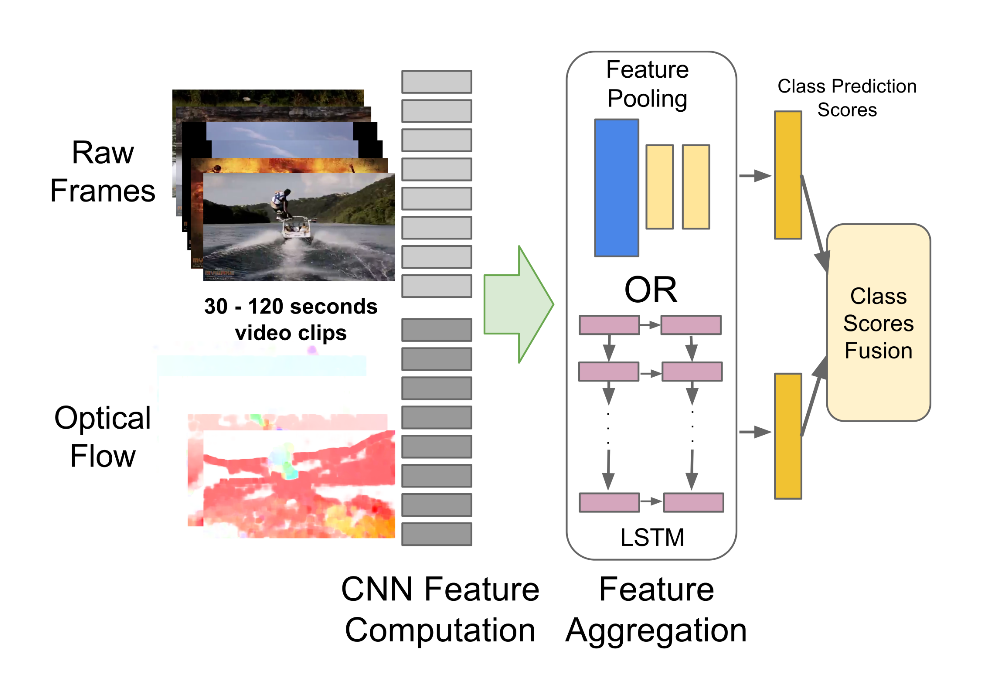
\includegraphics[width=0.6\textwidth]{img_deep/beyondshort_overview}
    \caption{Overview of the appraoch taken by \textcite{ng_beyond_2015}}
    \label{fig:beyondshort_overview}
\end{figure}

An advantage of this approach is that it can build on the achievements of CNN-based image processing architectures by directly embedding them as feature extractors for each frame.
Specifically two architectures are being evaluated for that:
\begin{enumerate}
    \item AlexNet \cite{krizhevsky_imagenet_2012}
    \item GoogLeNet \cite{szegedy_going_2015}
\end{enumerate}

Both networks take 220x220 pixel sized input images/frames.

The temporal extend of this approach can be easily adjusted by changing the number of CNNs that process an input frame each.

The CNNs for processing single frames all share paramters, which results in a constant number of trainable parameters over the number of input frames.

The authors propose to process input videos at only one frame per second, for being able to cover a long temporal extend while remaining computationally feasible.

Implicit motion information from processing adjacent frames is lost at this frame-rate.
This is compensated by using explicit motion information, i.e.\ optical flow inputs.

The Sports-1M and UCF-101 dataset are used as benchmarks in this work.

\textbf{Feature Pooling}\\
Pooling layers are used to combine feature vector representations of the input frames.

The authors consider, max-pooling, average pooling and a fully connected layer as pooling layers. Max-pooling results in faster learning architecture and was therefore chosen as the default pooling method in this approach. 

Several pooling architectures are evaluated (see figure \ref{beyondshort_poolingarchitectures}).

\begin{figure}[H]
    \centering
    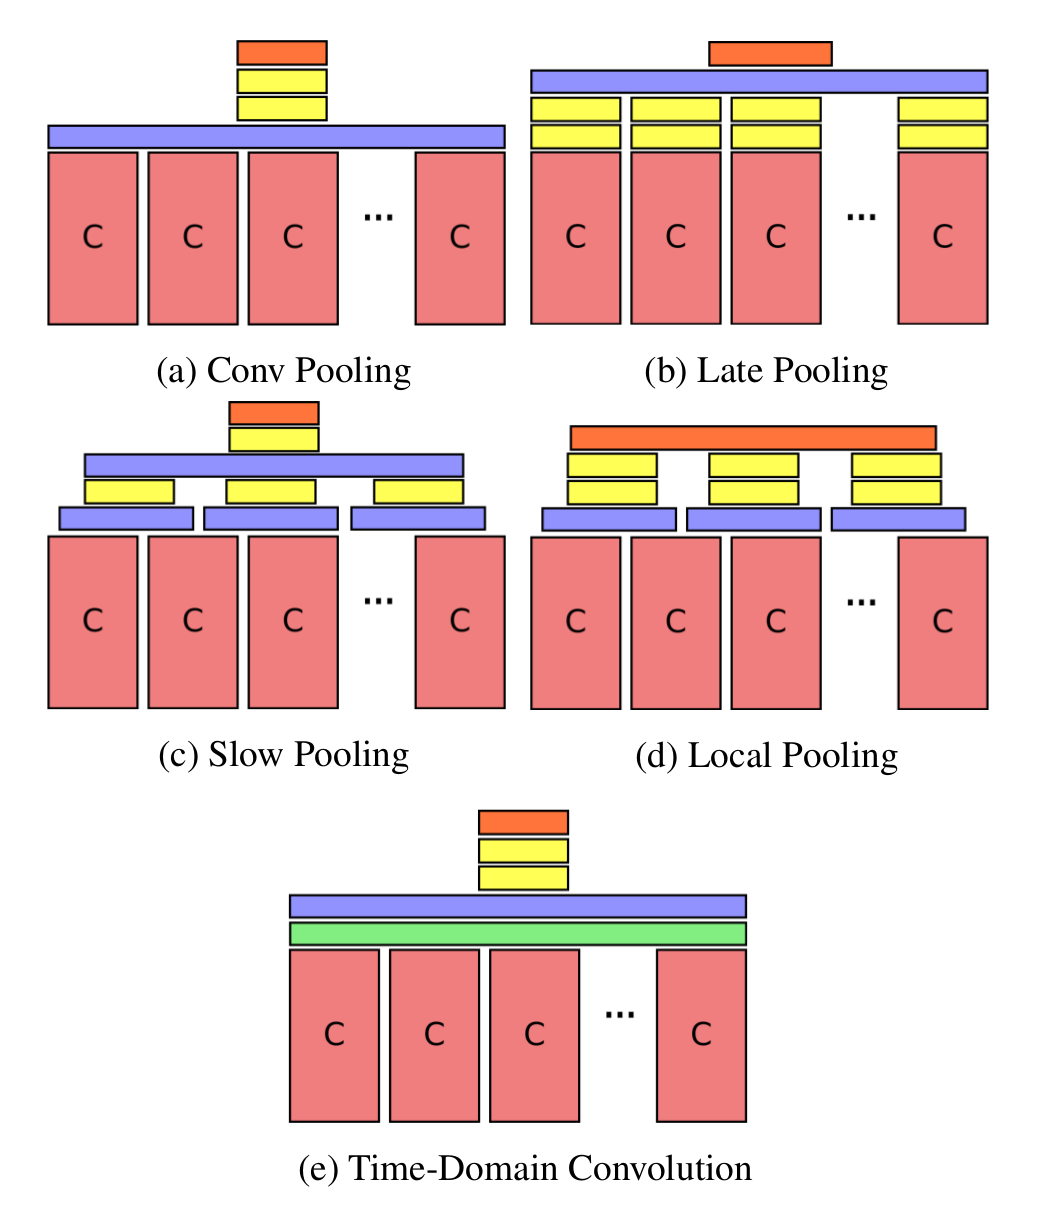
\includegraphics[width=0.5\textwidth]{img_deep/beyondshort_poolingarchitectures}
    \caption{Feature pooling architectures with: Max-pooling layers (blue), time-domain-convolution layer (green), fully-connected layers (yellow), softmax layers (orange). \cite{ng_beyond_2015}}
    \label{fig:beyondshort_poolingarchitectures}
\end{figure}

\begin{enumerate}[label=\alph*)]
    \item \textbf{Conv Pooling:} Max-pooling is performed over the activations of the final convolutional layers across all input frames.
    \item \textbf{Late Pooling:} Convolutional activations are first passed through two fully connected layers individually, before max-pooling is applied over the resulting high-level representations. Weights are shared between all convolutional and fully-connected layers.
    \item \textbf{Slow Pooling:} Two stages of pooling are applied: The first stage combines local temporal patches by max-pooling and feeds the activations into fully connected layers with shared weights. A single max-pooling layer then combines the resulting activations of all fully connected layers in the second stage.
    \item \textbf{Local Pooling:} Similar to slow pooling frame information is combined locally but only one stage of max-pooling is implemented. This prevents a potential loss of temporal information.
    \item \textbf{Time-Domain Convolution:} An additional time-domain convolutional layer is implemented before pooling features across frames.
\end{enumerate}

\textbf{LSTM architecture}\\
To capture the dynamic content, i.e.\ the information that is encoded in the differences between frames, a deep LSTM \cite{hochreiter_long_1997} architecture with 5 layers containing 512 memory cells each is used to aggregate sequences of frame-level CNN activations.

\begin{figure}[H]
    \centering
    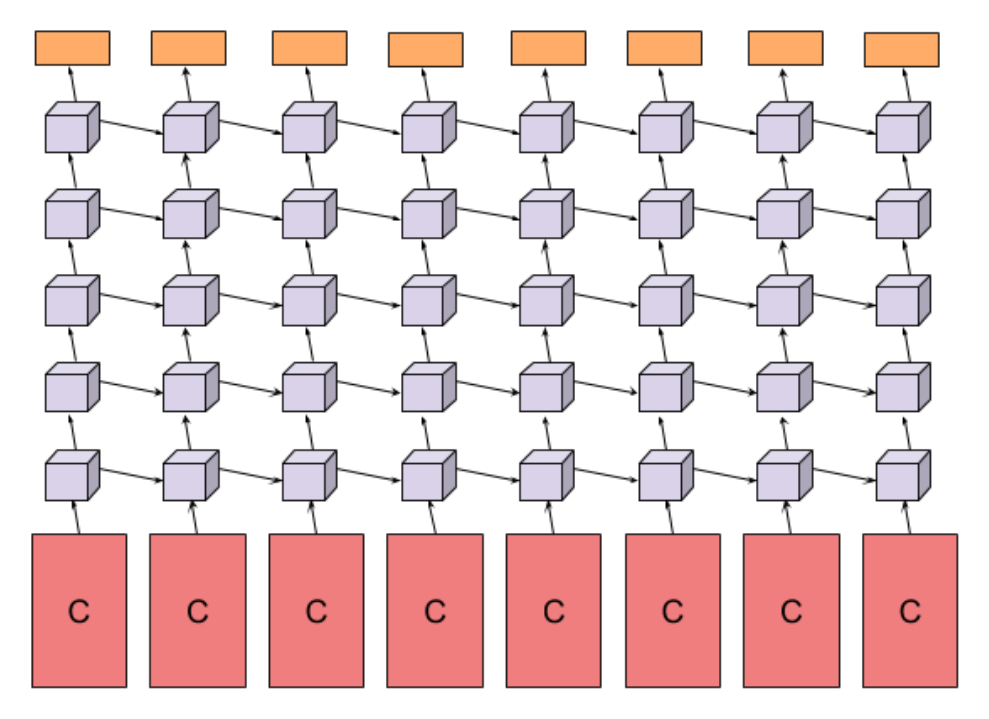
\includegraphics[width=0.6\textwidth]{img_deep/beyondshort_lstmarchitecture}
    \caption{LSTM Architecture. Five layers of LSTM cells take the final CNN activations as inputs. The video class is predicted at every timestep by a softmax output layer. \cite{ng_beyond_2015}}
    \label{fig:beyondshort_lstmarchitecture}
\end{figure}

The max-pooling architectures were trained on a computing cluster using a distributed version of Gradiend Descent Training called Downpour Stochastic Gradient Descent.

The AlexNet and GoogLeNet networks were initialized on pre-trained ImageNet models and then fine-tuned on the Sports-1M dataset in order to safe training time.

Since the CNN models share weights across input frames, the authors note that training time can also be saved by expanding a trained single-frame model to 30-frames and then expanding the 30-frames model to 120-frames.

Analogically to the two-stream approach of \cite{simonyan_two-stream_2014} the authors additionally train both their models on optical flow and perform late fusion over the two resulting streams.
The used optical flow is sampled at 15fps by using the method proposed in \cite{zach_duality_2007a}.

\textbf{Evaluation on Sports-1M dataset:}\\
For training and testing on Sports-1M, the first 5 minutes of each input-video are sampled at 1fps as input frames.

The frames are first resized to 256x256 pixels, a 220x220 pixel region of a randomly selected starting frame is selected and the following frames are cropped accordingly to create a network input of the desired temporal length.
Input frames are flipped horizontally with a probability of 50\%.

Models capable of processing 120 frames in a single example (which corresponds to 2 minutes of video) are trained.

240 random input examples are generated from a video for testing as described above and the predictions are averaged.

The LSTM models are not limited to a fixed input size and could generally process a complete video in a single pass.
The authors report a 3-5\% increase in Hit@1 accuracy when using the above mentioned data augmentation methods however.

As first result (see table \ref{tab:beyondshort_poolingevaluation}, the authors report the conv-pooling architecture to yield the best accuracy when evaluating different pooling methods.

\begin{table}[H]
    \centering
    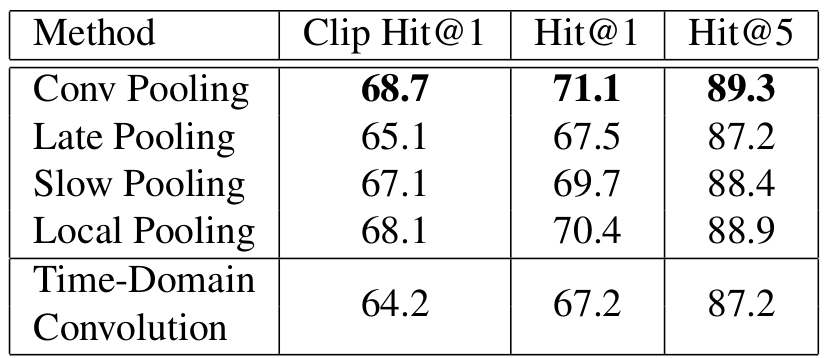
\includegraphics[width=0.5\textwidth]{img_deep/beyondshort_poolingevaluation}
    \caption{Evaluation of different pooling methods on Sports-1M dataset with a 120-frame AlexNet model. \cite{ng_beyond_2015}}
    \label{tab:beyondshort_poolingevaluation}
\end{table}

When evaluating the two different CNN architectures, GoogLeNet consistently outperforms AlexNet.
Fine tuning the models is noted to be crucial for high performance.

Evaluating the influence of the number of input frames confirmed the authors initial hypothesis, that longer sequences of an input video need to be considered for accurate action recognition.
The conv-pooling architecture with 120 input-frames yields a clip-hit of 70.8\%, which is an improvement of 70\% against the best clip-hit accuracy of \textcite{karpathy_large-scale_2014}. 
Results are shown in table \ref{beyondshort_framelengtheval}.

\begin{table}[H]
    \centering
    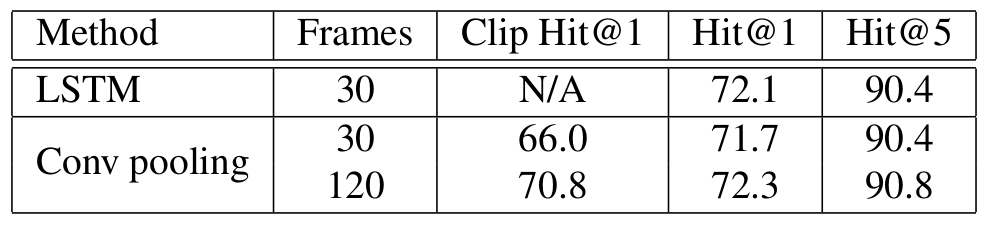
\includegraphics[width=0.6\textwidth]{img_deep/beyondshort_framelengtheval}
    \caption{Evaluation of the effect of the number of input frames using GoogLeNet CNN models. \textcite{karpathy_large-scale_2014}}
    \label{tab:beyondshort_framelengtheval}
\end{table}

When fusing 30-frame models with their optical flow counterparts, no significant increase in performance could be observed.
Also, the models trained on optical flow alone yield a much lower performance compared to training on still image frames.
The authors constitute this result to the noisyness of optical flow in the Sports-1M dataset (real-world videos with lower quality and rough cuts).

Yet overall, the best conv-pooling and lstm models perform significantly better than the state-of-the-art as reported by \textcite{karpathy_large-scale_2014}.

\textbf{Evaluation on UCF-101:}\\
The UCF-101 dataset contains short videos, lasting 10-15 seconds on average. It is therefore possible to extract frames at higher rates such as 6fps and still capture the complete input-video.

The authors compare frame sampling at different frame rates (30 fps and 6fps) for 30-frame models. They find, that decreasing the sampling rate from 30fps to 6fps slightly increases the classification accuracy, since the model captures more context from the input video (1 second of video against 5 seconds).

In comparison to the Sports-1M dataset, optical flow of UCF-101 provides an increase in performance.

The authors best models, which combine image frames and optical-flow, perform better by a small margin than the state of the art on UCF-101 reported by \textcite{simonyan_two-stream_2014}.

?? read conclusion!!


\subsubsection{Towards Good Practices for Very Deep Two-Stream ConvNets -- Wang et al. (2015)}
\cite{wang_towards_2015}

\textcite{wang_towards_2015} aim at improving the Two-Stream ConvNet approach for action recognition\cite{simonyan_two-stream_2014} by leveraging the advances of very deep ConvNet architectures in image classification.

The trends in network design that lead to the success of convolutional architectures in image classification are: smaller convolutional kernels, smaller kernel strides and deeper network architectures.

Examples of such very deep architectures are GoogLeNet\cite{szegedy_going_2015} and VGGNet\cite{simonyan_very_2014}.
The authors use these two models to train an enhanced Two-Stream ConvNet model for video action recognition.

The authors identify two main draw-backs of recent ConvNet approaches in video action recognition:
\begin{enumerate}
    \item The used models are shallow compared to their image counterparts. \\
        The deepest variant VGG-19 contains 16 convolutional layers, while the networks of the original Two-Stream ConvNet approach contain 5 convolutional layers.
    \item The available dataset are too small, which results in over-fitting.
\end{enumerate}

This work therefore proposes and evaluates a series of good practices to enable very deep ConvNet architectures for accurate action recognition, specifically in the two-stream ConvNet architecture.
These good practises namely are:
\begin{enumerate}
    \item Pre-training for the spatial- as well as the temporal-stream network.
    \item Smaller learning rates
    \item Different and more data augmentation techniques
    \item Higher drop-out ratios
\end{enumerate}

The two-stream ConvNet approach of \textcite{simonyan_two-stream_2014} uses pre-training on the ImageNet dataset for the spatial-stream network only and uses two convolutional networks with five convolutional layers each.

The authors name their approach Very Deep Two-Stream ConvNets.

The spatial net processes a single video frame of input size ($224 \times 224 \times 3$) and its architecture therefore is the same as in image classification, i.e.\ either GoogLeNet or VGGNet.

The temporal net processes 10 stacked optical flow fields splitted into images of the $x$- and $y$- coordinates.
Its input therefore has the size $224 \times 224 \times 20$ and the convolutional kernels in the first layer need to be different than in the spatial stream to process the higher-dimensional input.

Evaluations are done using the UCF101 dataset, specifically the three splits into training- and test-sets that are provided with it.
For each split, the training set consists of around 10.000 videos while the testing set consists of 3.000 videos.
UCF101 contains 13.320 videos in total and is considered extremely small for training very deep architectures.

\textbf{Pre-training}.
The spatial net is pre-trained using an ImageNet model as in \cite{simonyan_two-stream_2014}.
Specifically the network's weights are initialized with the values of a trained ImageNet model.

Interestingly, the authors find that pre-training is also beneficial for the temporal-stream network.
The authors average the ImageNet model's filters across channels and duplicate them 20 times as filters for the temporal net's first layer.

\textbf{Smaller dropout ratios}.
Since the networks in both streams have been pre-trained, the authors use smaller dropout ratios as in \cite{simonyan_two-stream_2014}.

The authors note a faster conversion of the training and credit this to the pre-training.

\textbf{Data Augmentation Techniques}.
Data augmentation techniques such as random cropping and horizontal flipping have been widely used to reduce over-fitting.

Since random cropping favors cropping regions in the center of an image/frame, the authors design a corner cropping strategy.
Specifically, they crop the four corners and the center of the input images.
This increases the variation of inputs and reduces over-fitting.

Additionally, network inputs are cropped from video frames on multiple scales.
The input video is first scaled to $256 \times 340$ pixels and the cropping width and height is randomly chosen from $\{256, 224, 192, 168\}$.
The cropped region is then scaled to $224 \times 224$ to form the network input.

\textbf{High Dropout Ratio}.
The authors use dropout ratios of 0.8 and 0.9 for the fully connected layers.

For testing 25 frames or optical flow fields are sampled from a test-video.
For each of these input instances 10 inputs to the very deep ConvNet are created by the above mentioned cropping method (four corners, the center and their horizontal flip).

The final prediction is obtained by averaging over all inputs.

Temporal and spatial net are fused using a weighted linear combination of both outputs.
The weight for the temporal net is set to $2$ and the weight for the spatial net is set to $1$.

Optical flow fields are extracted using the OpenCV implementation of TVL1 optical flow algorithm.

Table \ref{tab:towardsgood_results} shows the accuracy for the two evaluated very deep Two-Stream ConvNets.

\begin{table}[H]
    \centering
    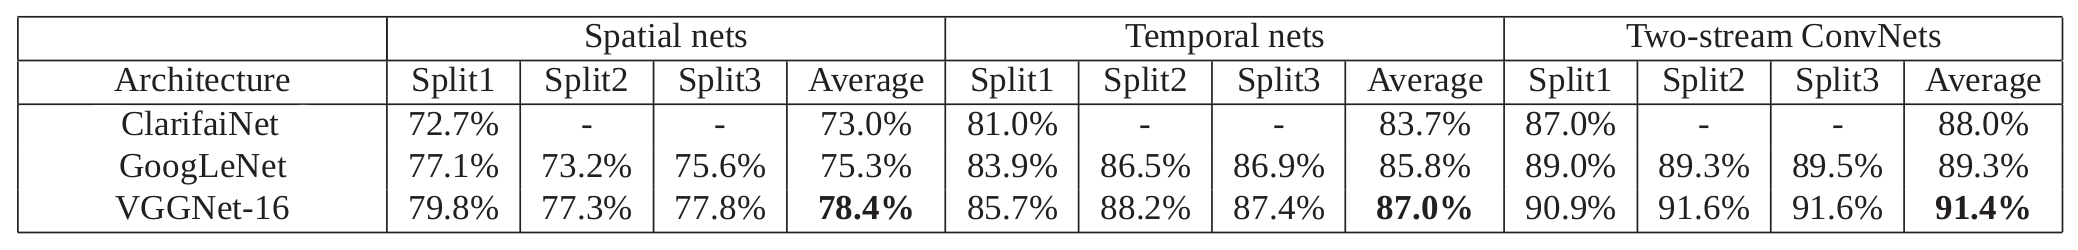
\includegraphics[width=\textwidth]{img_deep/towardsgood_results}
    \caption{Accuracy of the Two-Stream ConvNet architecture when building on different ConvNet models. Results for ClarifaiNet are taken from \cite{simonyan_two-stream_2014}, which isthe original two-stream approach. \cite{wang_towards_2015}}
    \label{tab:towardsgood_results}
\end{table}

The results show, that the proposed good practices and the employment of a very deep convolutional network lead to a significant improvement in performance over the original two-stream appraoch.


\subsubsection{Convolutional Two-Stream Network Fusion for Video Action Recognition -- Feichtenhofer et al. (2016)}
\cite{feichtenhofer_convolutional_2016}

\textcite{feichtenhofer_convolutional_2016} aim at improving the two-stream architecture for action recognition by addressing two main disadvantages of the approach:
\begin{enumerate}
    \item The architecture is not able to learn pixel-wise relations between the spatial stream and the temporal stream, i.e.\ it cannot relate extracted object-features to motion features, since the two separate streams are fused at the final softmax-layer. 
    \item A temporal extent of only $L = 10$ frames is processed by the temporal stream network in a single pass. Originally this was addressed by averaging network outputs over equally spaced temporal locations in the input video. However this averaging does not consider the temporal evolution of actions.
\end{enumerate}

The authors conduct a systematical evaluation of fusion methods to find a better way of combining the appearance information extracted by the spatial stream network with the motion information extracted by the temporal stream network.
More specifically, fusion techniques combine two feature maps of different ConvNets into a single feature map.
When combining all feature maps from a given convolutional layer with all the feature maps in the convolutional layer of another network, two network streams can be combined into one.

Fusion can be conducted either spatially or temporally.
Spatial fusion combines feature maps between the streams of the two-stream architecture. Temporal fusion combines feature maps resulting from applying the two-stream architecture on frames at different points of time in the input video.

In the original two-stream approach \cite{simonyan_two-stream_2014} fusion of the two streams is done by \textit{late fusion}, i.e.\ the two streams are combined by averaging the predictions of the softmax-output layer.

The authors evaluate temporal and spatial fusion methods and design an enhanced version of the two-stream architecture by implementing the best suited methods.

The objective of spatial fusion is to merge two networks after a given convolutional layer by combining the feature maps of the layers.

A fusion function $f: x^a, x^b \rightarrow y$ combines two feature maps $x^a, x^b \in \mathbb{R}^{W \times H \times D}$ into a fused feature map $y \in \mathbb{R}^{W \times H \times D'}$.
A feature map of a convolutional layer is given by the outputs of the neurons in the convolutional layer.
$W$ and $H$ corresponds to the spatial dimensions of the input frames, which get successively reduced by propagation through the layers.
$D$ and $D'$ correspond to the number of channels, i.e.\ the number of filters in the convolutional layer. 

\textbf{Sum Fusion}:\\
The sum of the activations in the two feature maps is computed at each location and used as the new feature map.
The output feature map has the same dimensions as the input feature maps.
Since the ordering of the channels is arbitrary in each network stream, this fusion technique does not implement a semantic relation between the feature maps.

\textbf{Max Fusion}:\\
This method is similar to Sum Fusion, but the maximum value at each location of the two feature maps is used as the new feature map.
The output feature map has again the same dimensions as the input feature maps and does not represesent a semantic relation between the feature maps.

\textbf{Concatenation Fusion}:\\
The two feature maps are stacked into each other along the dimesion of channels.
The resulting feature map has dimension $W \times H \times 2D$.
Since the activations are not combined by a mathematical operation, a relation between the feature maps is not implemented but it can be learned by the following layers.

\textbf{Conv Fusion}:\\
The feature maps are first concatenated as described above. A set of $D$ trainable filters with dimensions $1 \times 1 \times 2D$ is then convolved with the stacked feature maps and a bias is added to produce a resulting feature map of dimension $H \times W \times D$.
The convolution can be seen as a trainable weighted combination of the feature maps across the channels, which is able to learn semantic relations between two feature maps.

\textbf{Bilinear Fusion}:\\
The channel vectors of the feature maps at each pixel locations are combined by computing the matrix outer product of them. This results in $H \cdot W$ matrices for each pixel location which are then added to form the new feature map of dimension $D \times D$.
This fusion method is adapted from the Bilinear CNN approach in image classification \cite{lin_bilinear_2015a}.
Usually the fully connected layers are replaced by a linear SVM to make this fusion method usable in practice, i.e.\ the compensate the high number of parameters.

Implementing a layer that performs spatial fusion between two network streams has significant influence on the number of trainble parameters in the network, especially if the networks are fused before the fully connected layers and if only the merged stream is kept. Most of the parameters are located in the fully connected layers.

In figure \ref{fig:streamfusion_layerplacement} two examples of placing fusion layers into the two-stream architecture are shown.

\begin{figure}[H]
    \centering
    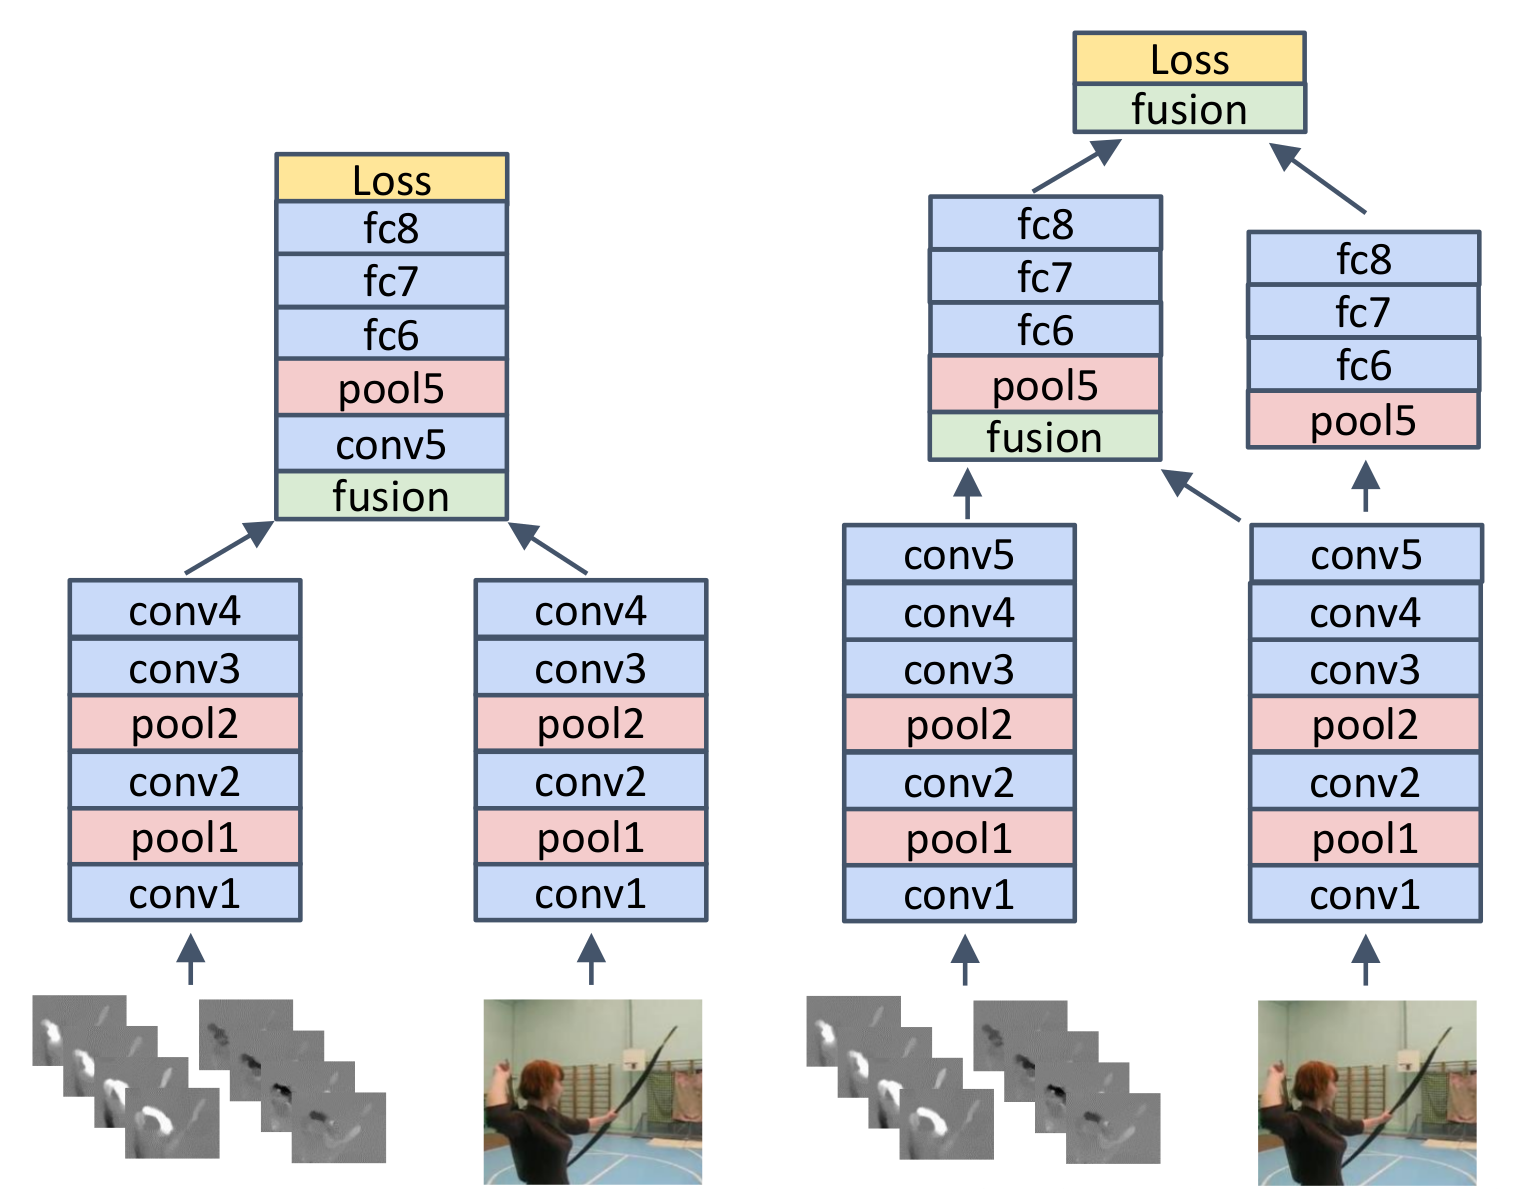
\includegraphics[width=0.75\textwidth]{img_deep/streamfusion_layerplacement}
    \caption{Placement examples of fusion layers for early combination of the spatial and temporal stream in two-stream architectures. (\textit{left}) Only the merged stream is kept. (\textit{right}) The spatial stream is kept after the first fusion layer and fused into it before the final layer \cite{feichtenhofer_convolutional_2016}}
    \label{fig:streamfusion_layerplacement}
\end{figure}

The authors evaluate the spatial fusion methods in a two-stream architecture as implemented in the original approach \cite{simonyan_two-stream_2014}.
Each stream consists of 5 convolutional layers, and three fully connected layers.
The accuracy on UCF101 (Split1), the number of paramters and overall number of layers in the architecture is given in table \ref{tab:parameternumber}.
The streams are fused after the rectification of the fifth convolutional layer and only the fused stream is kept.

\begin{table}
    \centering
    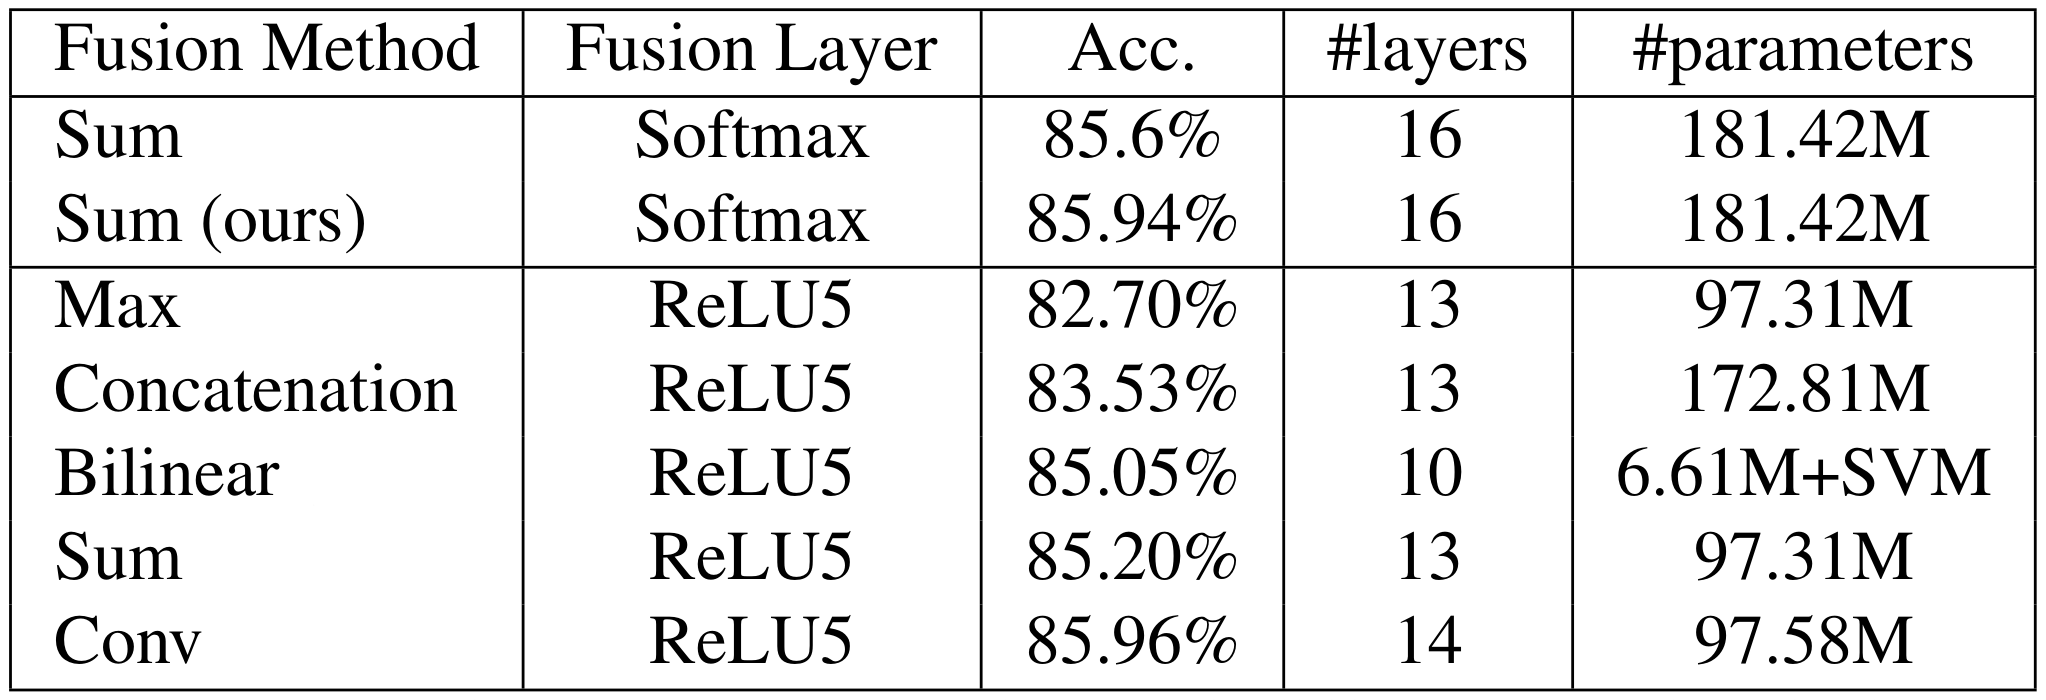
\includegraphics[width=0.5\textwidth]{img_deep/streamfusion_parameternumber}
    \caption{Performance and number of parameters for different spatial fusion methods in a two-stream setup, evaluated on UCF101 (split 1) \cite{feichtenhofer_convolutional_2016}}
    \label{tab:streamfusion_parameternumber}
\end{table}

Results of the origignal approach are reported in the first row.
As can be seen the authors' approach yields comparable results, when implementing the same fusion method.
Conv Fusion performs best and reduces the number of parameters significantly to roughly half of the parameters in the original approach.

Implementing the fusion layer after an earlier convolutional layer decreses the performance significantly.
Best results are obtained by fusion after the rectification layer of convolutional layer 5, keeping both streams and fusing again at the final layer (as shown in figure \ref{fig:streamfusion_layerplacement} (right)).

After evaluating spatial fusion methods, the authors evaluate temporal fusion methods.
In order to fuse feature maps temporally, they are considered to be extended over time by applying the two-stream architecture at several temporal points across the video and stacking the resulting feature maps.

The input to a temporal pooling layer is a feature map $x \in \mathbb{R}^{H \times W \times T \times D}$ where $H$ and $W$ again correspond to the spatial location, $T$ corresponds to the temporal dimension, i.e.\ the number of feature maps that get stacked and $D$ again corresponds to the number of channels in the feature map, i.e.\ the number of filters in the convolutional layer.

\begin{figure}[H]
    \centering
    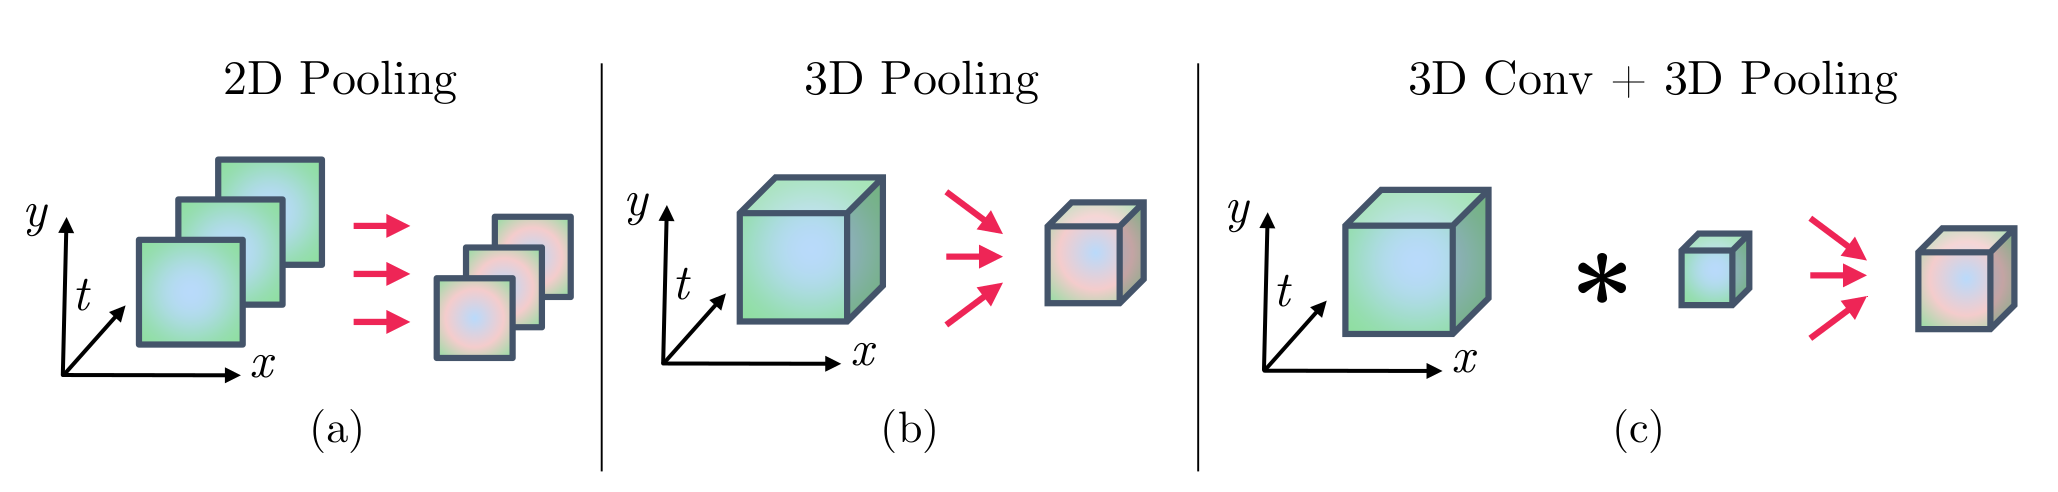
\includegraphics[width=\textwidth]{img_deep/streamfusion_temppooling}
\caption{Methods for pooling feature maps along the temporal dimension. \cite{feichtenhofer_convolutional_2016}}
    \label{fig:streamfusion_temppooling}
\end{figure}

\textbf{(a) 2D pooling.}
The feature maps in each channel are only pooled spatially.
The network predictions are averaged over all the outputs for different points in time, where the network has been applied.
The pooling operation ignores the temporal dimension.

\textbf{(b) 3D pooling.}
Max-pooling with a 3D pooling filter of dimensions $W' \times H' \times T'$ is applied to the stacked feature maps.
The max-pooling operation executed for each of the channels $D$ individually.
Pooling across different channels is not conducted.

\textbf{(c)3D Conv + 3D Pooling.}
A set of $D'$ filters $f \in \mathbb{R}^{W'' \times H'' \times T'' \times D \times D'}$ is convolved with the stacked feature maps and biases are added.
The resulting feature map is then pooled with a 3D pooling filter as described above.
Since the convolutional filter is trainable, it is able to learn weighted combinations of features in a local spatio-temporal region.

The authors evaluate the pooling methods and find that 3D Conv + 3D Pooling performs best.

The final approach for applying the two-stream ConvNet model to action recognition is implemented by the authors as follows:


Take away message in abstract.

\subsection{Trajectory Pooling of Deeply Learned Features}

\subsubsection{Action recognition with trajectory-pooled deep-convolutional descriptors -- Wang et al. (2015)}
\textcite{wang_action_2015} propose a novel method of building video representations by combining the advantageous porperties of hand-crafted features as in \textit{Dense Trajectories} \cite{wang_action_2013} with deeply learned features as in \textit{Two-Stream Convolutional Networks} \cite{simonyan_two-stream_2014}.

In the \textit{Improved Dense Trajectories} approach, local features are extracted along trajectories, which are mostly located near prominent motion in a video.
The authors claim however, that hand-crafted features are not discriminative enough for accurate action recognition.

Deep architectures have proven to learn discriminative features effectively with \textit{Two-Stream Networks} being a successful approach that finally performed comparably to \textit{Improved Dense Trajectories}.

The main outline of the approach for action recognition is as follows:
\begin{enumerate}
    \item A two-stream convolutional network architecture is trained on multiple scales of a large dataset.
    \item \textit{Dense Trajectories} are begin extracted from the input video according to the approach in \cite{wang_action_2013}.  
    \item The deeply learned feature maps of the two-stream architecture are used to extract local descriptors, by pooling the convolutional responses over areas around the trajectories. The resulting descriptor is called Trajectory-pooled deep-convolutional descriptor (TDD). ??
    \item The local TDDs are aggregated over the complete video using the Fisher Vector representation. cite ??
    \item A linear SVM is trained to assign the action label to the FV representations, i.e.\ to perform action recognition.
\end{enumerate}

The authors evaluate their approach on the HMDB51 and UCF-101 dataset. Results show, that TDD is complementary to HOG, HOF and MBH and therefore fusion of these descriptors can further boos performance.

In contrast to \cite{wang_action_2013}, trajectories are only extracted on the original spatial scale, because it is computationally more effective.
To compensate, multi-scale TDDs are extracted around the trajectories.

Any convolutional architecture can be embedded in a two-stream setup for TDD extraction.
The authors choose the Clarifai network \cite{zeiler_visualizing_2014-1} with less filters in the \textit{conv4} layer (512 instead of 1024) and a lower dimensional \textit{full7} layer (2048 instead of 4096).
Architectural details are depicted in table \ref{tab:tdd_layers}) below.

\begin{table}[H]
    \centering
    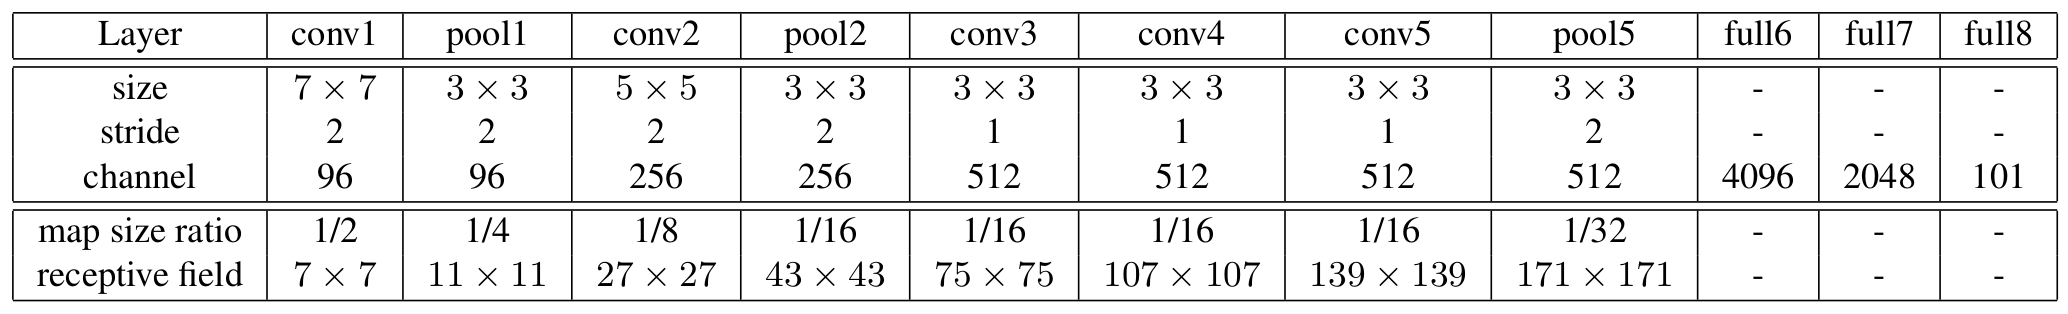
\includegraphics[width=\textwidth]{img_deep/tdd_layers}
    \caption{Layers of the Clarifai network modified for TDD extraction \cite{wang_action_2015}}
    \label{tab:tdd_layers}
\end{table}

This architecture is chosen for implementing the spatial stream network as well as the temporal stream network.

After training of the two-stream architecture, the activations of the convolutional layers in each stream (feature maps) are used for extracting the TDD descriptors of an input video.

Before each convolutional or pooling layer with kernel size $k$, zero padding of the layer's input is applied with size $\lfloor k/2 \rfloor$.
This padding prevents an additional reduction in dimensionality between the layer's input and output besides the reduction that stems from applying the kernel with a certain stride.
Therefore the position of a trajectory point in the input can be easily related to coordinates in the convolutional feature map at question by incorporating the map size ratio $r$ of the layer (see table \ref{tab:tdd_layers}).
Specifically, the $p$-th point in a video trajectory $(x_p, y_p, z_p)$ is represented by point $(\overline{r \times x_p}, \overline{r \times y_p}, z_p)$.
Where $\overline{(.)}$ denotes the mean-value.

Given a video $V$, training of the two-stream architecture results in a set of feature maps $\mathbb{C}(V)$ from the spatial stream $s$ and temporal stream $t$.
\begin{equation*}
    \mathbb{C}(V) = \{C_1^s, C_2^s, \cdots, C_M^s, C_1^t, C_2^t, \cdots, C_M^t\}
\end{equation*}
where:
\begin{itemize}
    \item $C_m^s, C_m^t \in \mathbb{R}^{H_m \times W_m \times L \times N_m}$ denotes the $m$-th feature map of the spatial or temporal stream
    \item $H_m$ is it's height
    \item $W_m$ is it's width
    \item $L$ is the number of video frames
    \item $N_m$ is the number of channels
    \item $M$ is the number of feature maps in each stream.
\end{itemize}

There are two steps involved in extracting the local trajectory-aligned descriptor called TDD from a 3D volume around a trajectory:
\begin{enumerate}
    \item Feature Map Normalization (two different methods)
        \begin{itemize}
            \item Spatiotemporal Normalization
            \item Channel Normalization
        \end{itemize}
    \item Trajectory pooling
\end{enumerate}

\textbf{Normalization}
Normalization has been widely applied to hand-crafted features beacause it reduces the influence of illumination.
The authors use this technique on convolutional feature maps to suppress the activation burstiness of some neurons.

In Spatiotemporal Normalization, each feature map is normalized independently across each channel according to it's maximal value.
Specifically, for any channel $n$ and a feature map $C \in \mathbb{C}(V)$:
\begin{equation*}
    \tilde{C}_{st}(x,y,z,n) = C(x,y,z,n) / \max_{x,y,z} C(x,y,z,n)
\end{equation*}
This normalization method ensures, that the feature maps across all channels range in the interval $(0,1)$.

In Channel normalization the values of each feature map are normalized according to the values at the same spatial positions but in another channel.
Specifically, for an spatial position $(x,y,z)$ in the feature map at question:
\begin{equation*}
    \tilde{C}_{ch}(x,y,z,n) = C(x,y,z,n) / \max_{n} C(x,y,z,n)
\end{equation*}
This normalization method ensures, that the feature map values of each pixel range in the interval $(0,1)$ and therefore contribute equally to the final representation.

Both normalization methods were evaluated experimentally and the authors found, that combining the resulting video representations from both normalization methods by late fusion yields the best results.

\textbf{Trajectory Pooling}
Given the $k$-th trajectory out of all trajectories $\mathbb{T}(V)$ over a video $V$, a trajectory-pooled deep convolutional descriptor in respect to a normalized feature map $\tilde{C}_m$ is constructed by sum-pooling the feature map values along the trajectory-points in the feature map.

\begin{equation*}
    D(T_k, \tilde{C}_m) = \sum_{p=1}^P \tilde{C}(\overline{(r_m \times x_p^k)}, \overline{(r_m \times y_p^k)}, z_p^k)
\end{equation*}
Where $r_m$ is the map size ratio belonging to feature map $\tilde{C}_m$.

The extracted TDDs over a complete video are then aggregated using the Fisher Vector representation cite ?? to form a global video representation.
A linear SVM is then trained to learn the action classes to these representations.

\begin{figure}[H]
    \centering
    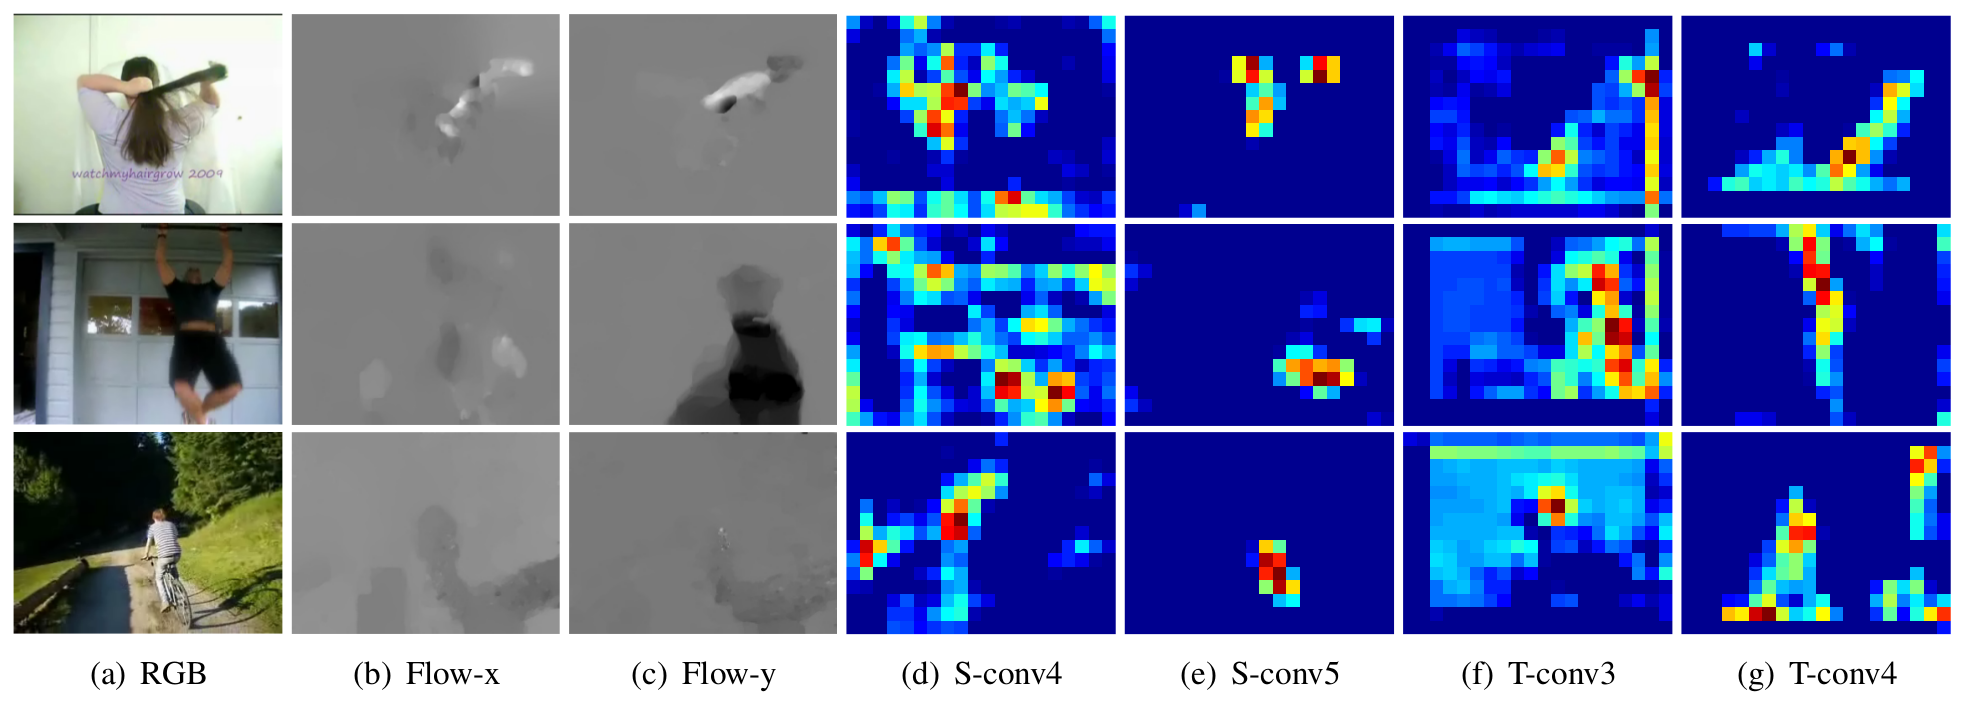
\includegraphics[width=\textwidth]{img_deep/tdd_featuremaps}
    \caption{Snapshots of input videos (a), their corresponding optical flow fields in $x$- and $y$-dimension (b - c), the corresponding activations of the feature maps used for TDD extraction (d - g) \cite{wang_action_2015}}
    \label{fig:tdd_featuremaps}
\end{figure}

Using TDDs for action recognition is evaluated on the UCF-101 and HMDB-51 datasets. Since UCF-101 is bigger than HMDB-51, the authors initially train the two-stream model on the bigger UCF-101 dataset and transfer it for TDD extraction on HMDB-51.

The weights of the \textbf{Spatial Net} are initialized using the publicly available model of \cite{chatfield_return_2014} and then fine-tuned on the frames of UCF-101 videos.
During fine-tuning, the frames of UCF-101 are first resized to have 256 pixels on their smallest side.
A randomly cropped region of $224 \times 224$ pixels then builds the network training input after random horizontal flipping.

The \textbf{Temporal Net} is trained from scratch on stacked optical flow image volumes.
The optical flow between two adjacent frames of a training-video is calculated using the TVL1 algorithm \cite{zach_duality_2007} (implemented in OpenCV) and split into images of it's $x$- and $y$- component.
This forms the optical flow volume for the complete video.
A $224 \times 224 \times 20$ pixel sized sub-volume is randomly cropped from it and randomly flipped to form a training-input for the temporal stream network.

The authors evaluate the two-stream architecture without extracting TDDs and obtain similar results as \textcite{simonyan_two-stream_2014}.

Experimental evaluation shows, that using the descriptors from \textit{conv4} and \textit{conv5} in the spatial net as well as from \textit{conv3} and \textit{conv4} in the temporal net yields best performance in action recognition.

Combining the descriptors of the spatial and temporal net in the TDD approach significantly outperforms the previous state of the art (two-stream convolutional network \cite{simonyan_two-stream_2014}).
Quantitative results are shown in table \ref{tab:tdd_results}.

\begin{table}[H]
    \centering
    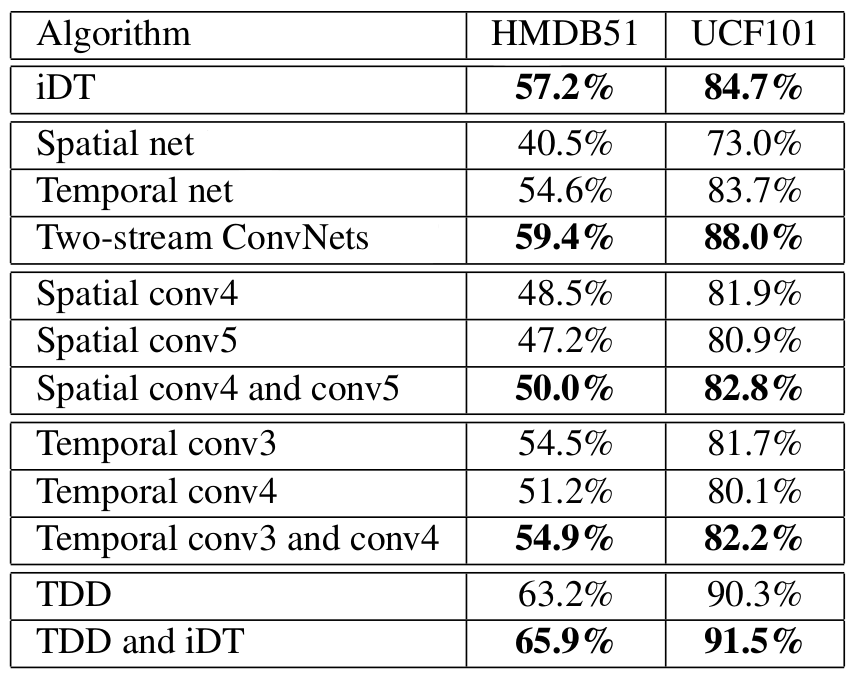
\includegraphics[width=0.5\textwidth]{img_deep/tdd_results}
    \caption{Action recognition performance of TDDs on HMDB51 and UCF101 compared to improved dense trajectories (iDT) \cite{wang_action_2013} and two-stream ConvNets \cite{simonyan_two-stream_2014}. \cite{wang_action_2015}}
    \label{tab:tdd_results}
\end{table}


\subsubsection{?Pooling the Convolutional Layers in Deep ConvNets for Action Recognition -- Zhao et al. (2015)}
\cite{zhao_pooling_2015}


\subsection{Generative Models}

One of the most popular deep learning models that can be trained unsupervised is the restricted Boltzmann machine [5]. A nice property of RBMs is that they can be greedily trained and stacked on top of each other to form deep belief networks (DBNs) [6], allowing us to learn representations of gradually increasing complexity. Training of these models using maximum likelihood learning is intractable, but they can be trained using contrastive divergence [4]. (Palasek Patras)

\textbf{Auto-Encoders:}\\
The most common architecture used is an auto-encoder
which learns representations based on its ability to recon-
struct the input images [35, 3, 49, 37]. Wang an Gupta (Unsupervised learning of visual representations using video.

\textbf{Restricted Boltzmann Machine:}\\
Boltzmann Machines are probabilistic networks, specifically undirected graphical models, that can learn the probability distribution inherent in a given dataset.
A Boltzmann Machine consists in its simplest form of two binary layers: A visible layer $x$ and a hidden layer $h$, which are fully connected to each other.
The Boltzmann Machine allows connections between units of the same layer, which renders training computationally extremely demanding.

The design of the Restricted Boltzmann Machine addresses this problem by restricting connections to nodes between different layers, which explains its name.
Restricted Boltzmann Machines can be trained using a Markov Chain Monte Carlo algorithm, namely Contrastive Divergence.

Once a Boltzmann Machine is trained, i.e.\ it learned the underlying probability distribution, data can be sampled from it.
The visible layer functions as both, input-layer during training and output-layer during sampling.

Restricted Boltzmann Machines can be trained with labeled as well as unlabeled data (supervised or unsupervised).

When training in an unsupervised manner, the RBM is able to learn feature representations of the inputs by mapping them onto its hidden layer.
\ldots

When labeled data is present, the RBM can perform classification. 
For training, the labels are being concatenated with the input data and fed into the RBM.
A prediction for a given test example can then be obtained by using it as input for the RBM and sampling the model for the missing input, that was used for the labels during training.
The RBM then generates the most likely value for the missing label-input given the testing-input.

Restricted Boltzmann Machines correspond to feed-forward neural network models when reusing the learned weights in a topological equivalent NN model.
This is how unsupervised pre-training is conducted.

Models that can be trained in an usupervised manner are especially attractive for the video-domain where labeling data is costly.

The RBM can be extended to process real-valued inputs.

Deep Belief Networks are stacked Restricted Boltzmann Machines.
In general the learning capacity of a single RBM is limited, but it can be increased by stacking multiple RBMs to form so called Deep Belief Network. (Lee)

\subsubsection{Unsupervised Learning of Video Representations using LSTMs -- Srivastava et al. (2015)}
\cite{srivastava_unsupervised_2015}

\textcite{srivastava_unsupervised_2015} design models based on Long-Short-Term-Memory (LSTM) recurrent neural networks and evaluate their ability to learn representations of input videos in an unsupervised way from unlabeled video data.
Similar to the approach taken in auto-encoders, an encoder LSTM network maps input sequences of vectors into a fixed-length representation, which is then decoded by another LSTM network into a target sequence.
The authors consider different choices for the target sequence: the reversed input sequence, a sequence of future frames after the input ended or a hybrid approach where two LSTM networks decode the representation into both these choices simultaneously.
Inputs to the LSTM encoder-network can be any kind of video representation, the authors evaluate raw image patches and high level "percepts" that are extracted by a CNN.

The results of the unsupervised setting are evaluated qualitatively by printing the decoded sequences. For a quantitative evaluation, the unsupervisedly pre-trained models are fine-tuned for an supervised action recognition task on the UCF-101 and HMDB-51 dataset.

Three different types of models are being evaluated, which are described below.
\begin{enumerate}
    \item LSTM Auto-encoder model.
    \item LSTM Future Predictor model.
    \item A Composite (hybrid) model.
\end{enumerate}

The \textbf{LSTM Auto-encoder model} consists of an encoder and a decoder LSTM network.
The encoder network is presented with one vector of the input sequence per timestep.
After the final input has been processed, the encoder network's state is used as the representation of the input.
The decoder network is then trained to translate the representation back into the initial input sequence, but in reverse order.
If the decoder is able to reconstruct the input sequence accurately from the representation, all needed information about the input sequence must be encoded in the representation (which therefore is a good representation).

The model is depicted in figure \ref{fig:unsupervisedlstms_autoencoder}.

\begin{figure}[H]
    \centering
    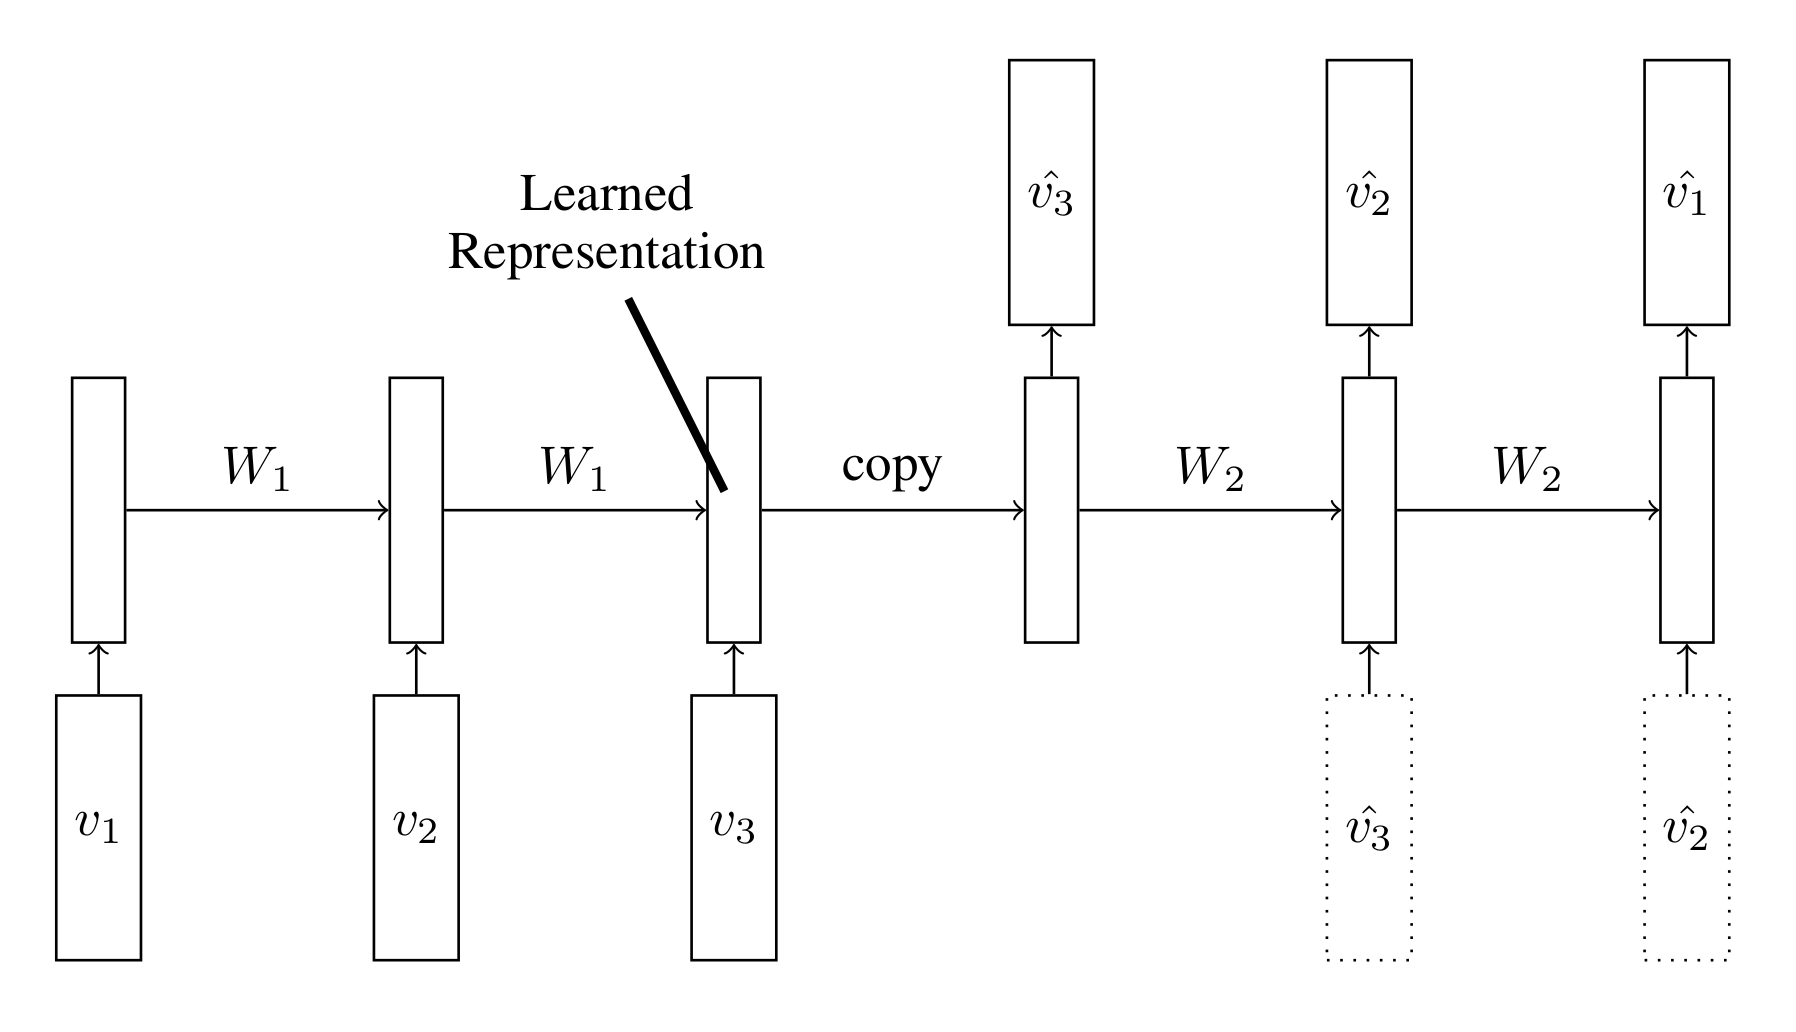
\includegraphics[width=0.75\textwidth]{img_deep/unsupervisedlstms_autoencoder}
    \caption{Auto-encoder model \cite{srivastava_unsupervised_2015}}
    \label{fig:unsupervisedlstms_autoencoder}
\end{figure}

$W_i (i \in \mathbb{N})$ denotes the parameters of the respective LSTM network that are, according to its recurrent nature, applied to its own hidden state given an input $v_i$ of the input sequence $\{v_1, \cdots, v_T\}$ of length $T$.
$\hat{v}_i (i \in \mathbb{N})$ denotes the outputs of the decoder network.
The decoder network can be conditional, i.e.\ it receives its last generated output as input.

The \textbf{LSTM Future Predictor model} also consists of two LSTM networks but predicts frames that continue after the input sequence.
The architecture is the same as in the Auto-encoder model, as shown in figure \ref{fig:unsupervisedlstms_futurepredictor}.
This decoder LSTM network can again be unconditioned or conditional.

\begin{figure}[H]
    \centering
    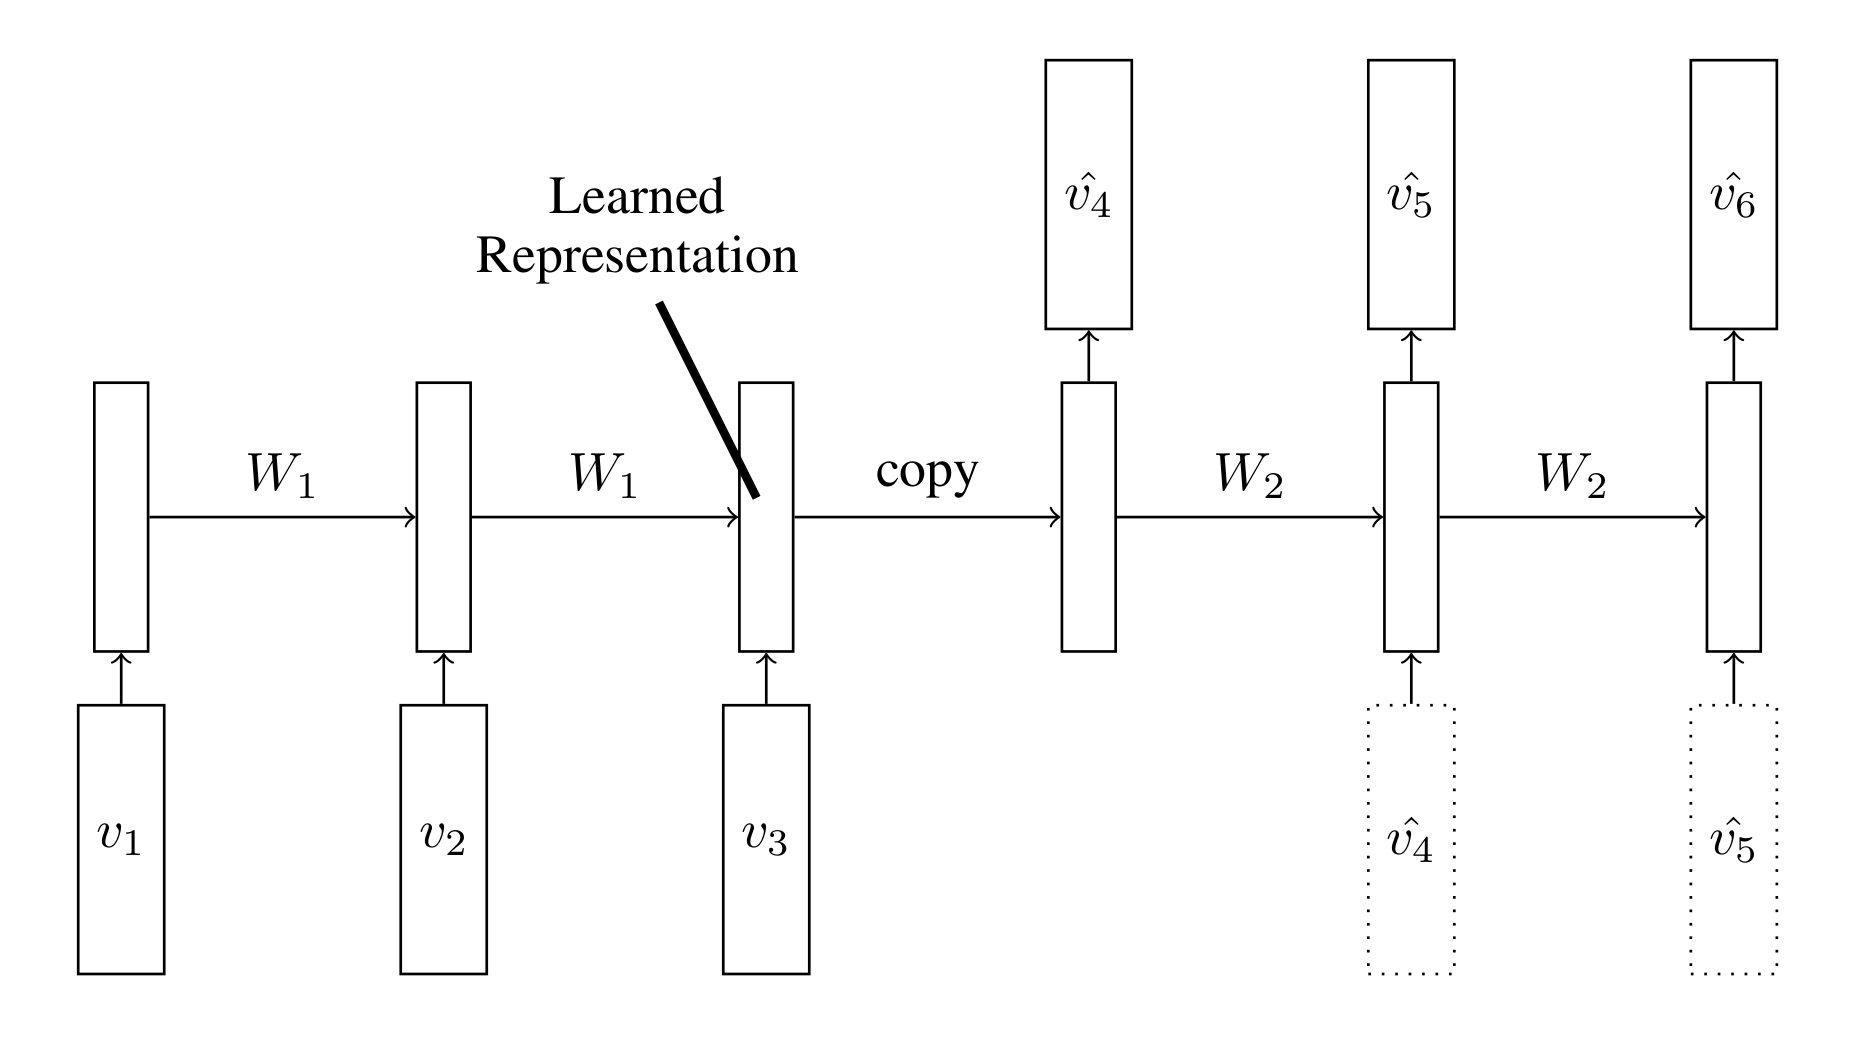
\includegraphics[width=0.75\textwidth]{img_deep/unsupervisedlstms_futurepredictor}
    \caption{Future-predictor model \cite{srivastava_unsupervised_2015}}
    \label{fig:unsupervisedlstms_futurepredictor}
\end{figure}

The \textbf{Composite model} consists of an encoder LSTM network and two decoder LSTM networks, which reconstruct the original input sequence and predict future frames simultaneously.
This model tries to overcome the disadvantages that each of the single models have: A high-capacity auto-encoder tends to simply memorize the inputs, while a future predictor tends to store information about just the last few frames of the input, because those are needed most for future prediction.
The composite model, as shown in figure \ref{fig:unsupervisedlstms_composite}, therefore puts the additional constraint on the encoder networ, that its representation must allow both tasks.

\begin{figure}[H]
    \centering
    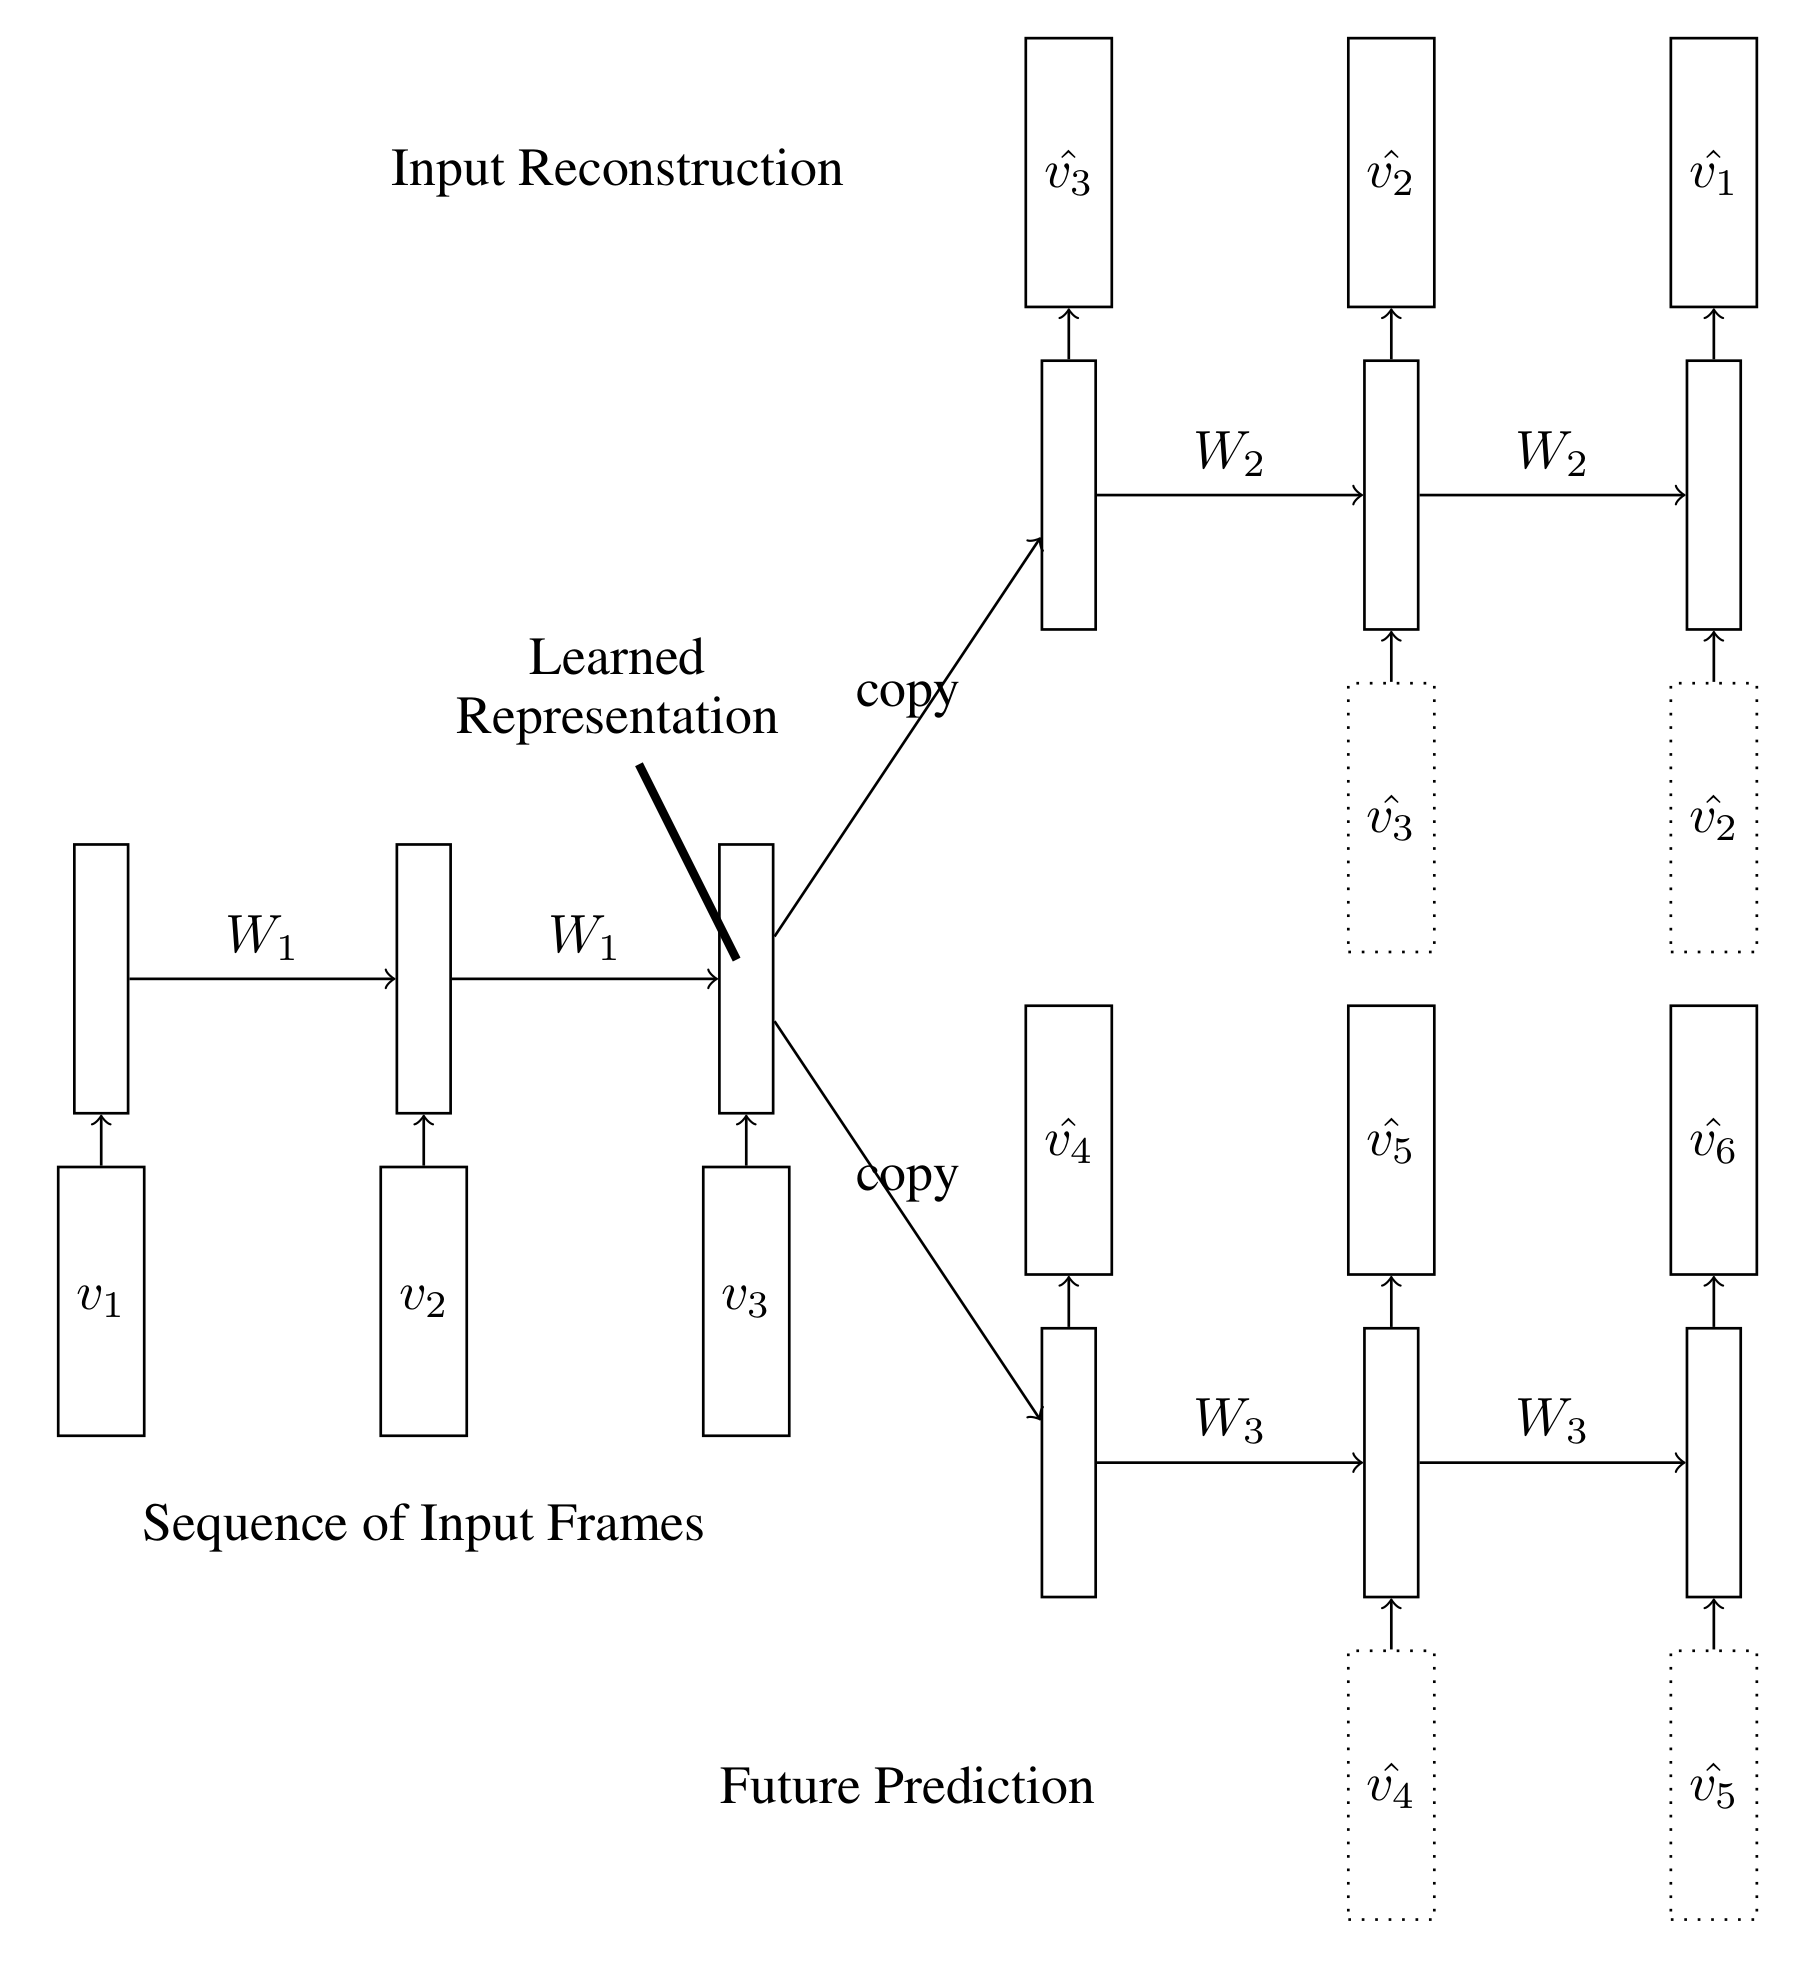
\includegraphics[width=0.75\textwidth]{img_deep/unsupervisedlstms_composite}
    \caption{Composite model \cite{srivastava_unsupervised_2015}}
    \label{fig:unsupervisedlstms_composite}
\end{figure}

The authors provide a qualitative analysis of the properties of their proposed models through visualization.
First composite models, with one and two layers consisting of $2048$ LSTM units, are trained on a syntethic dataset of two moving MNIST digits in a $64 \times 64$ pixel area.
The results for image reconstruction and future prediction shown in figure \ref{fig:unsupervisedlstms_movingmnist}.

\begin{figure}[H]
    \centering
    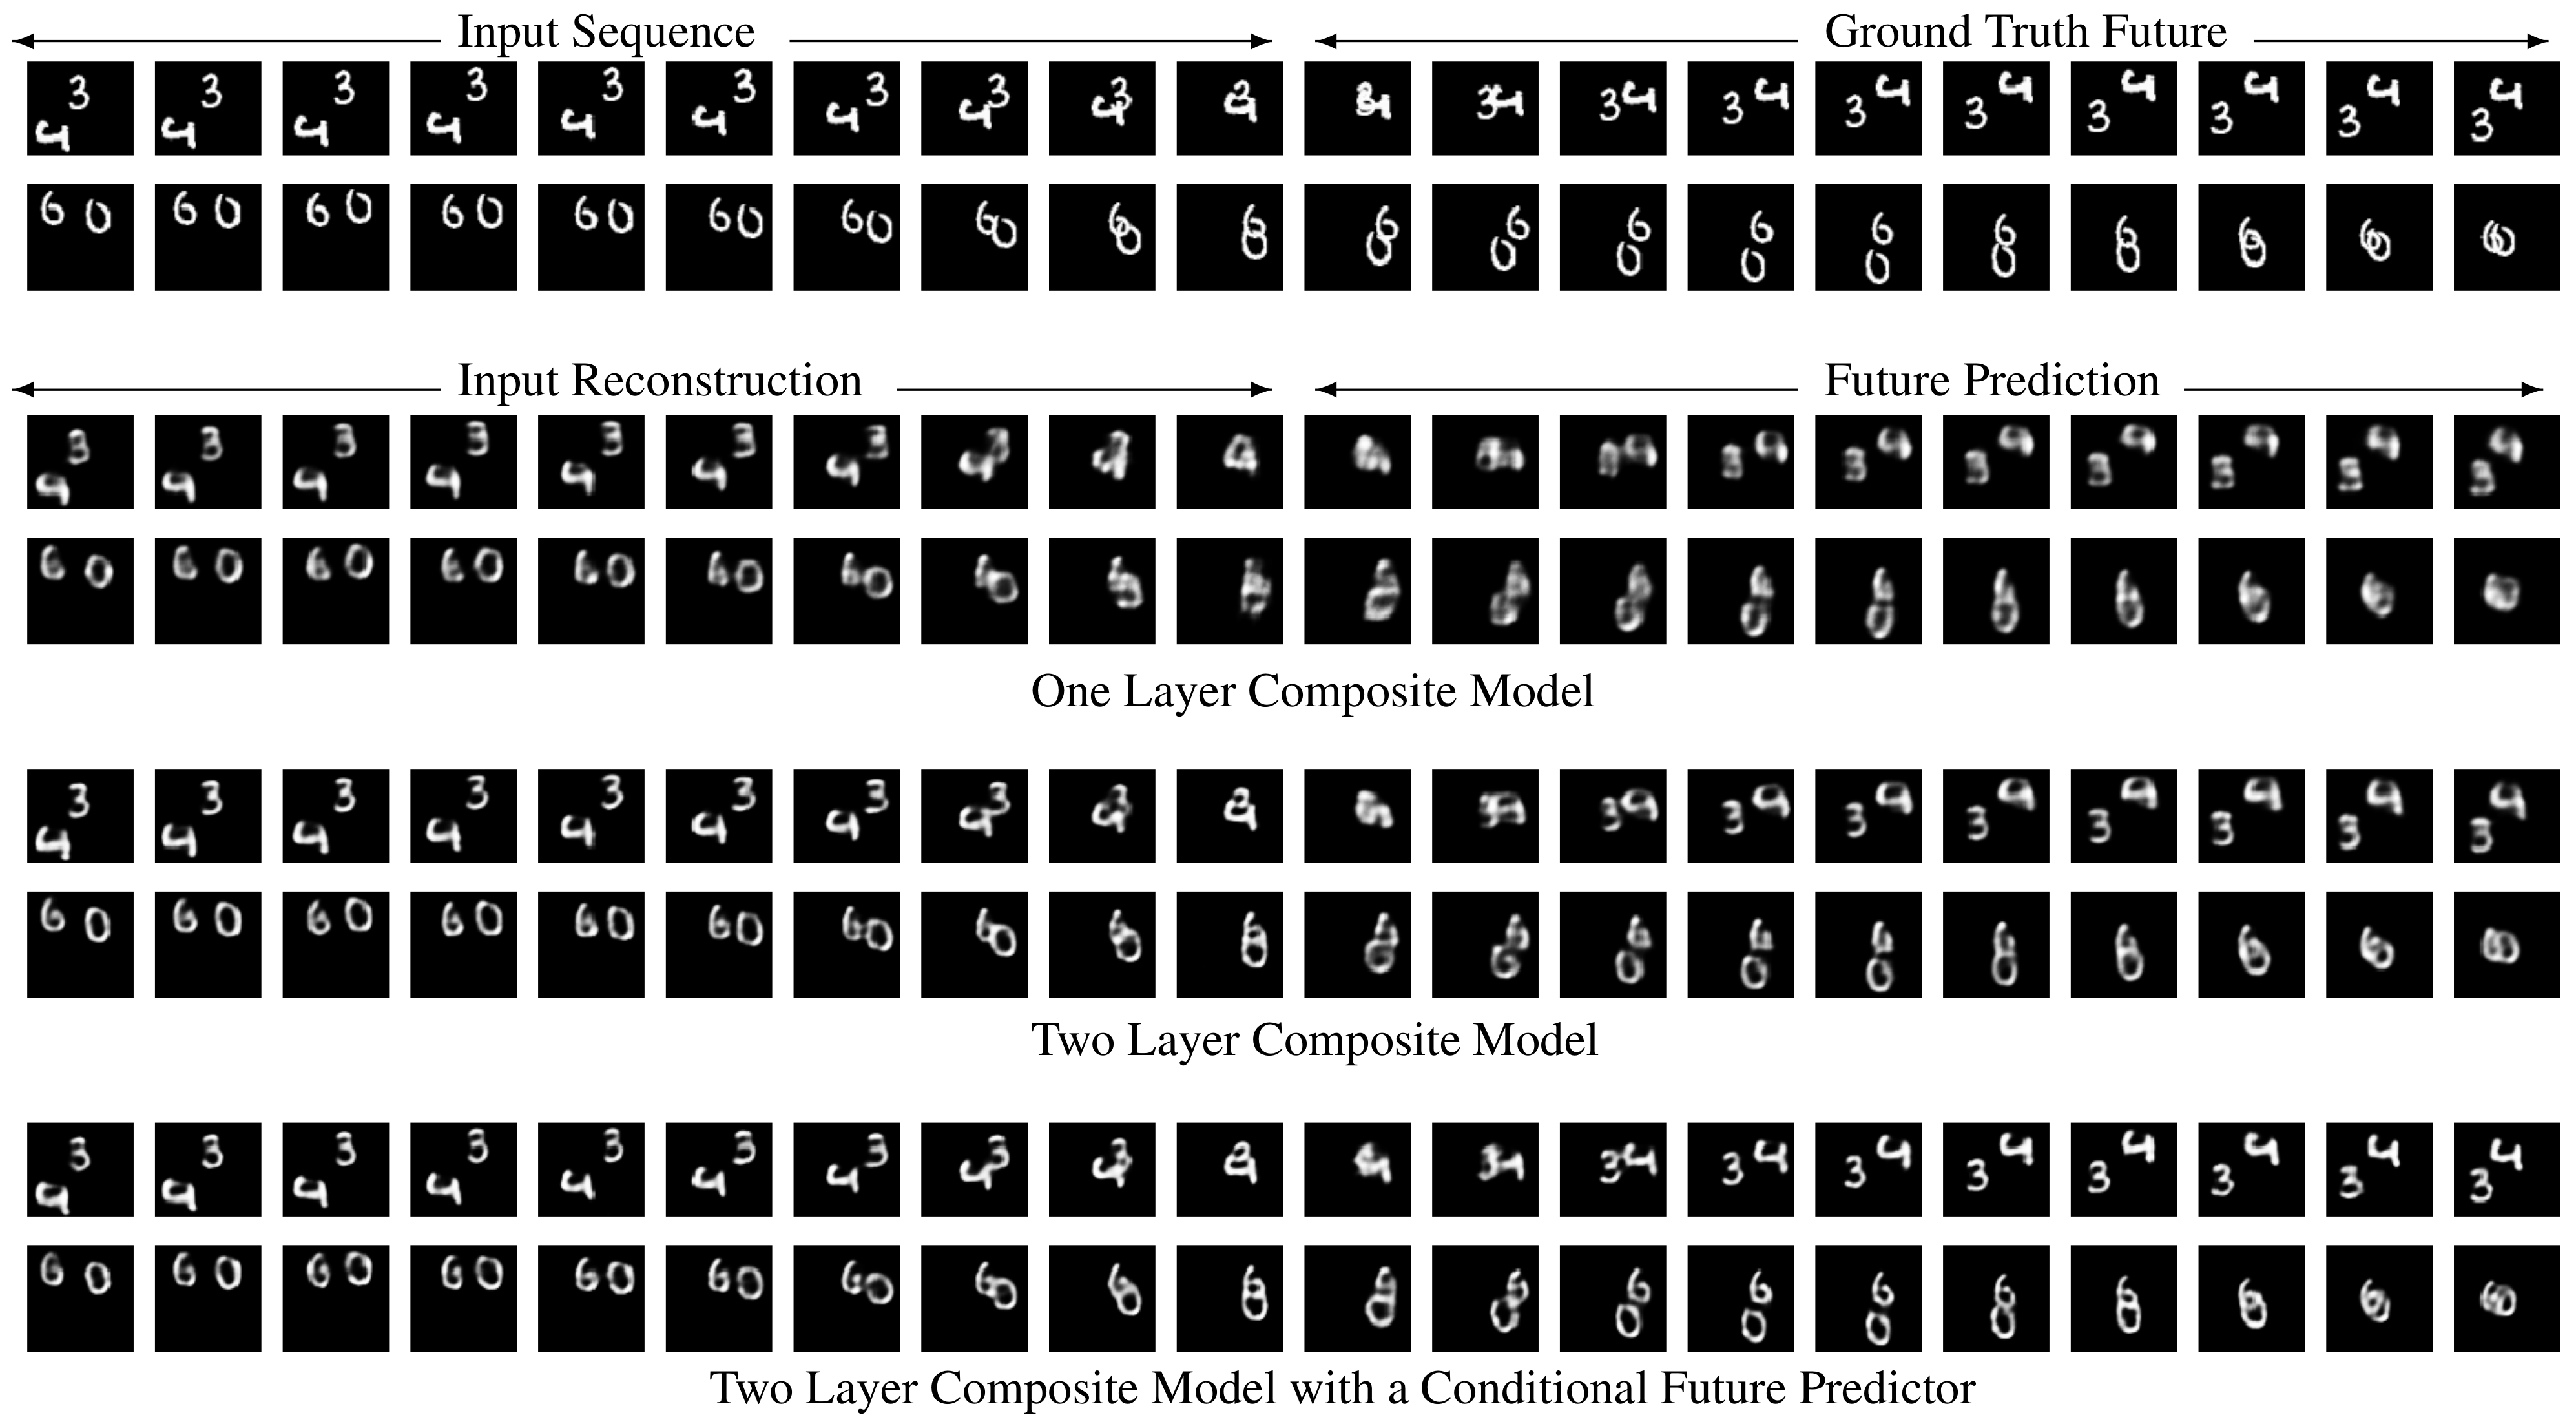
\includegraphics[width=\textwidth]{img_deep/unsupervisedlstms_movingmnist}
    \caption{Input reconstruction and future predictions of composite models on a synthetic dataset of moving MNIST digits. \cite{srivastava_unsupervised_2015}}
    \label{fig:unsupervisedlstms_movingmnist}
\end{figure}

These results show, that the model is able to make fairly good predictions on this dataset.
Adding a second layer and making the future predictor conditional further improves the predictions.

When applying the model on $32 \times 32$ image patches of real-life videos from the UCF-101 dataset, results show, that the future prediction quickly blurs out.

\begin{figure}[H]
    \centering
    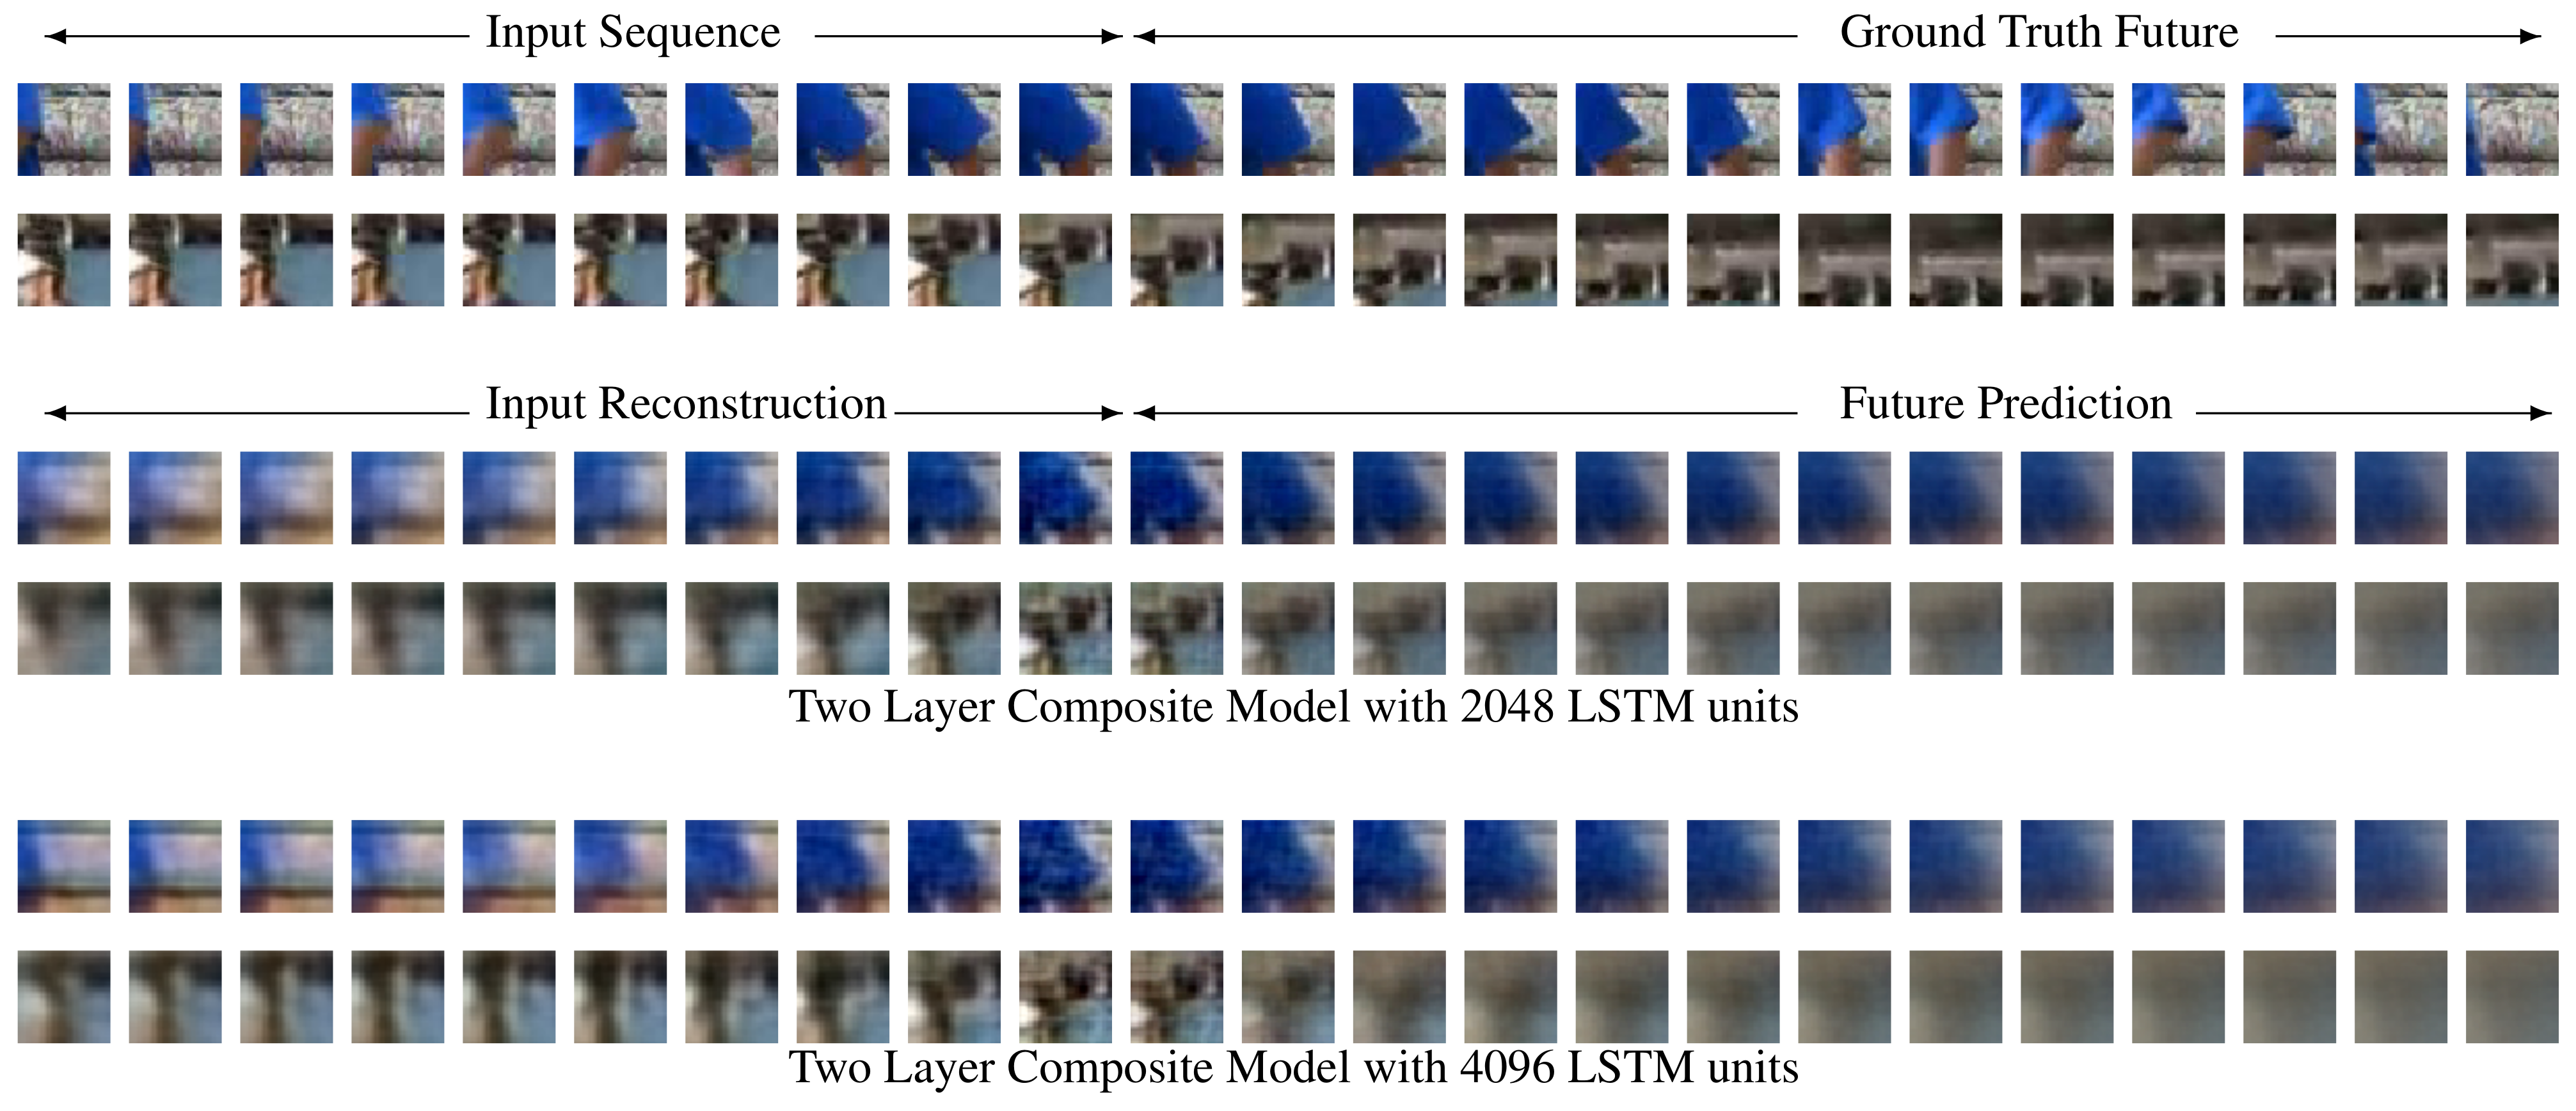
\includegraphics[width=\textwidth]{img_deep/unsupervisedlstms_ucfpatches.png}
    \caption{Image reconstruction and future prediction of a two-layer composite model with a different number of LSTM units in each layer. \cite{srivastava_unsupervised_2015}}
    \label{fig:unsupervisedlstms_ucfpatches}
\end{figure}

The authors evaluate if features obtained from unsupervised learning can increase the accuracy in supervised action recognition:
A two layer composite model is trained in an unsupervised way on 300 hours of video, composed of 10 seconds clips randomly sampled from the Sports-1M dataset.
Once trained, a LSTM classifier is initialized with the weights of the encoder network (figure \ref{fig:unsupervisedlstms_classifier}).
Depending on the used benchmark, this classifier is then fine-tuned using backpropagation on either UCF-101 or HMDB-51.
The model is designed to use center crops of size $224 \times 224$ from the datasets or high-level optical-flow percepts, i.e.\ activations of a temporal stream CNN as in \cite{simonyan_two-stream_2014}, as inputs.

\begin{figure}[H]
    \centering
    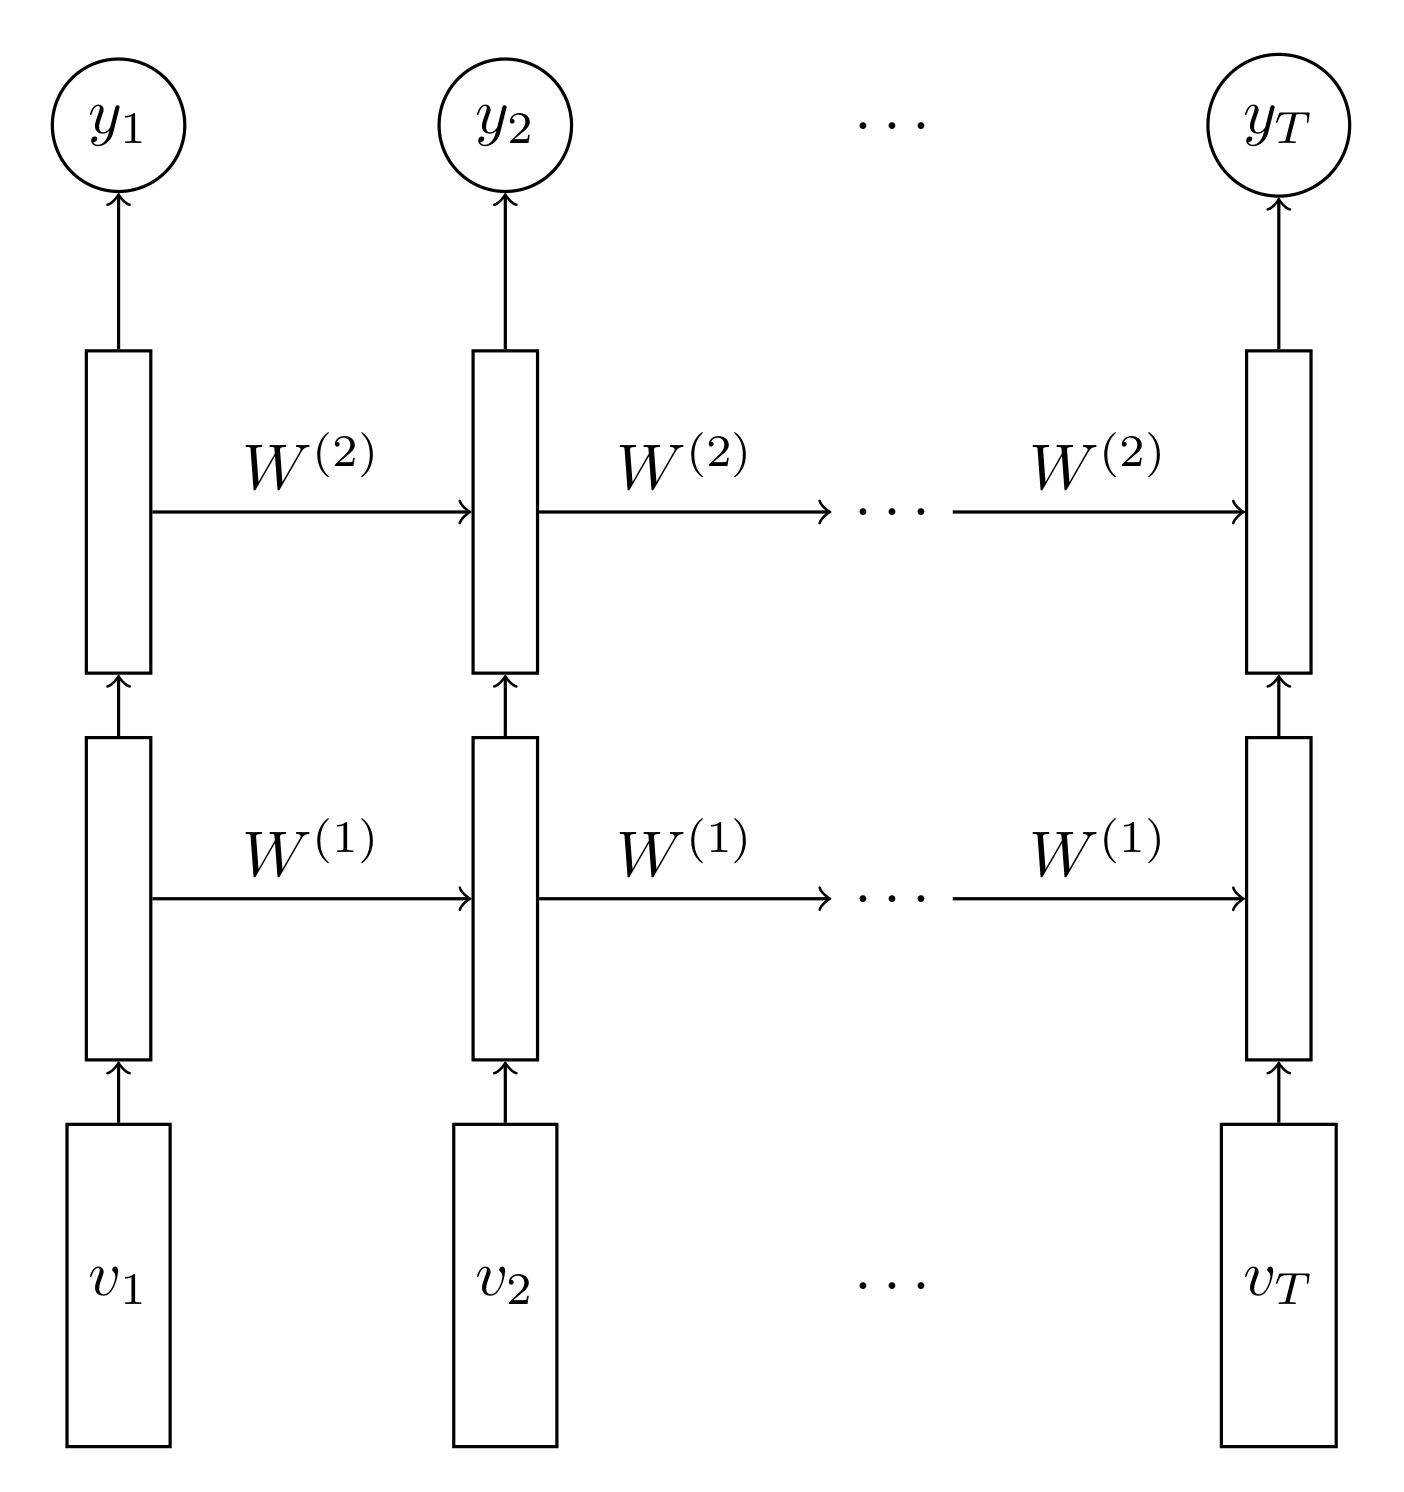
\includegraphics[width=0.5\textwidth]{img_deep/unsupervisedlstms_classifier}
    \caption{LSTM classifier applied on an input sequence $\{v_1, \cdots, v_T\}$ \cite{srivastava_unsupervised_2015}}
    \label{fig:unsupervisedlstms_classifier}
\end{figure}

Baseline method is initializing the model with random weights.
The results show, that initializing the model with features obtained from unsupervised learning increases the performance significantly, when only very few training examples per class are available (improvement of about $5\%$).
With more available labeled data, the improvement becomes smaller (about 1\%).

The authors conclude: Even models pretrained on unrelated datasets (300 hours of YouTube videos) can help action recognition performance.
Unsupervised learning gives a significant improvement if only few training examples are available.


\subsubsection{Action Recognition Using Convolutional Restricted Boltzmann Machines -- Palasek and Patras (2016)}
\cite{palasek_action_2016}

\textcite{palasek_action_2016} apply Convolutional Deep Belief Networks (ConvDBNs), which are generated by stacking Convolutional Restricted Boltzmann Machines (ConvRBMs), to static video frames to learn video representations for human action recognition in an unsupervised fashion.

The ConvRBM was initially proposed by \textcite{lee_convolutional_2009-1} to address several problems that occur when applying RBMs and DBNs to images:
\begin{enumerate}
    \item Realistic images are high-dimensional and DBNs do not scale well with the input size. \cite{lee_convolutional_2009-1} 
    \item DBNs do not take the special structure of images into account, specifically that objects can occur in any area of the image. Features therefore have to be learned for each location in the image separately. \cite{lee_convolutional_2009-1} 
\end{enumerate}

Equivalently to Convolutional Neural Networks, the Convolutional Restricted Boltzmann Machine uses weight-sharing and pooling to make the detection of a specific feature in an input image translationally invariant.

The basic ConvRBM architecture is shown in figure \ref{fig:convrbm_architecture}.
The visible layer $V$ is constituted of binary input units, but can be easily modified to handle real-valued inputs.
The hidden layer consists of $K$ groups, with a filter $W^k$ belonging to each group ($k \in \{1,\cdots, K\}$).
To illustrate the equivalency to other translational invariant architecture such as CNNs, which consists of detection and pooling layers, the hidden layer is denoted as detection layer in Figure \ref{fig:convrbm_architecture}.
A group corresponds to a feature map in CNNs, i.e. the activations produced by a convolutional filter.
The filter weights define the connections between a local patch in the visible layer and a hidden unit in the detection layer of the filter's group.
All hidden units in the detection layer of a group are connected to their local patches by the same filter weights.
The hidden units share a bias $b_k$ per group and all visible units have a single bias $c$.
\cite{lee_convolutional_2009-1}

\begin{figure}[H]
    \centering
    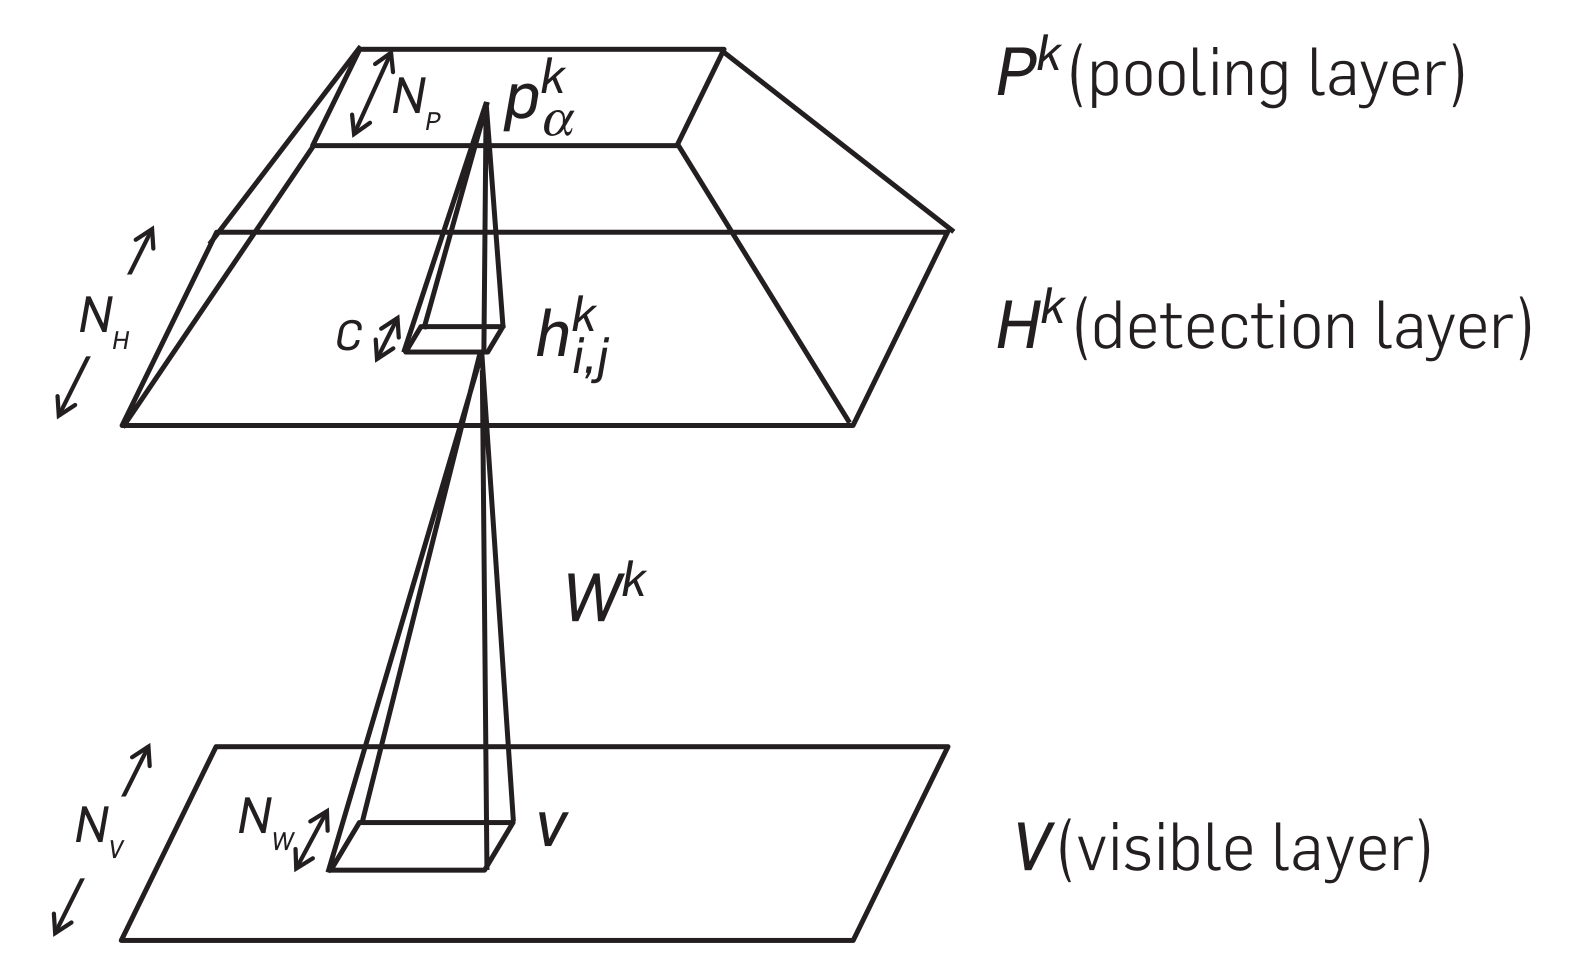
\includegraphics[width=0.6\textwidth]{img_deep/convrbm_architecture}
    \caption{Architecture of the Convolutional Restricted Boltzmann Machine. The figure shows group $k$ in the detection- and pooling-layer. \cite{lee_convolutional_2009-1}}
    \label{fig:convrbm_architecture}
\end{figure}

ConvRBMs are stacked above each other to form a more expressive deep architecture, called Convolutional Deep Belief Networks (ConvDBNs).
Equivalently to Convolutional Neural Networks, probabilistic max-pooling is used to reduce the dimensionality of each hidden (detection) layer.
Since regular max-pooling was designed for deterministic models, \textcite{lee_convolutional_2009-1} derive a probabilistic max-pooling method, in order to enable full probabilistic inference in their model.
In probabilistic max-pooling, only one unit in the input patch of the pooling operation is allowed to be active.
The output unit is active, if and only if one unit in the input patch is active.
Pooling operations are needed, to feed progressively more information to higher-level feature detectors and to make high-level representations invariant to translations of features in the lower layers. \cite{lee_convolutional_2009-1}

The energy function of the ConvDBN is defined by summing the energy functions of the individual ConvRBMs.
ConvDBNs are trained in a greedy, layer-wise way: After a layer is trained individually, its weights are frozen and its activations in the hidden/detection layer are taken as inputs for the following layer.
\cite{lee_convolutional_2009-1}

\textcite{palasek_action_2016} devise and evaluate an approach for using the activations of three stacked ConvRBMs (a ConvDBN) for action recognition.
They use the Gaussian-Bernoulli version of ConvRBMs, which is the real-valued extension of regular binary ConvRBMs, to extract features from still video patches and aggregate them into a video representation that can be classified using a SVM.

Different configurations for the ConvDBN are being evaluated as feature extractors:
\begin{description}
    \item[1.\ layer ConvRBM] \hfill \\
        Either $32$ or $64$ filters sized $5 \times 5$ or $3 \times 3$ pixels.\\
        Optional probabilistic max-pooling layer with patch size of $2 \times 2$ units.
    \item[2.\ layer ConvRBM] \hfill \\
        Contains $64$ filters of size $3 \times 3$
        Optional probabilistic max-pooling layer with patch size of $2 \times 2$ units.
    \item[3.\ layer ConvRBM] \hfill \\
        Contains $128$ filters of size $3 \times 3$ pixels.
        Optional probabilistic max-pooling layer with patch size of $2 \times 2$ units.
\end{description}

The approach for generating fixed length video representations for variable sized input videos is shown in \ref{fig:palasekpatras_approachschematik}.

\begin{figure}[H]
    \centering
    \includegraphics[width=0.9\textwidth]{img_deep/palasekpatras_approachschematik}
    \caption{Approach for generating fixed sized video-representations using ConvDBN activations. An input video is handled as video-volume of stacked frames. \cite{lee_convolutional_2009-1}}
    \label{fig:palasekpatras_approachschematik}
\end{figure}

Given an input video, video subvolumes of size $32 \times 32$ pixels and of length $15$ subframes are extracted at random positions in the video-volume.
Each subframe is fed individually into the ConvDBN and the resulting activations of one of its layers are extracted.
The activations of all subframes are stacked to form a feature representation of the subvolume.
This feature representation is then divided into $2 \times 2 \times 3$ parts, mean-pooled anlong the temporal dimension, spatially pooled and concatenated to form the final representation of the given subvolume (see figure \ref{fig:palasekpatras_approachschematik}). \cite{lee_convolutional_2009-1}

A Gaussian Mixture Model is trained on all the extracted feature representations to extract the final Fisher Vector representation of the video.
These Fisher Vector can then be classified using a SVM.
 
Their model is unsupervisedly trained on greyscaled, static video-frames of the UCF-101 dataset, which contains a total of $1700000$ frames.
For each of the 9537 videos in split 1 of the UCF-101 dataset, $1000$ subvolumes are extracted to train the ConvDBN in an unsupervised way.

\textcite{palasek_action_2016} evaluated their approach using activations from different ConvDBN layers.
Activations from the first pooling layer worked best and yield an accuracy of $55.06\%$ in the overall approach.
Although, the results are not competitive to other state-of-the-art approaches reported previously in this work, the experiments were conducted to compare the performance of features learned in an unsupervised manner to hand-crafted features.
The authors also evaluated incorporating HOG features in their experimental setup and achieved significantly worse results: $50.75\%$.
They therefore argue, that features learned in an unsupervised way are more descriptive than hand-crafted features for human action recognition from video.
\cite{lee_convolutional_2009-1}

\subsection{Temporal Coherency Networks}
``Temporal Coherency is a form of weak supervision and states that consecutive frames are correlated both semantically and dynamically.'' going deeper into action recognition.

Previous unsupervised approaches only yielded moderate increase in accuracy against initializing the weights randomly.

Misra:
Example tasks: Ordering of frames, determining the relative temporal proximity of frames.

%\subsubsection{Unsupervised learning of spatiotemporally coherent metrics -- Goroshin et al. (2015)}
%cite{goroshin_unsupervised_2015}


%subsubsection{Unsupervised learning of visual representations using videos -- Wang and Gupta (2015)}
%cite{wang_unsupervised_2015}


\subsubsection{Shuffle and Learn: Unsupervised Learning using Temporal Order Verification -- Misra et al. (2016)}
\cite{misra_shuffle_2016}

\textcite{misra_shuffle_2016} propose an efficient unsupervised representation learning method based on temporal order verification.

Temporal order verification is a binary classification task. Given a sequence of video frames, a classifier has to determine whether the sequence is in correct temporal order.
Datasets to train and test such a classifier can be easily generated by drawing short sequences of frames from a video and switching frames in a subset of all sampled sequences.

In the strictest sense, using temporal order verification for representation learning is not an unsupervised method, since the labels \textit{correct temporal order} and \textit{incorrect temporal order} are learned for input sequences.
The authors argument however, that obtaining the label is free and the method can therefore be attributed as unsupervised.

Learning the validity of a sequence of frames yields a representation that captures the motion of persons and objects in the scene. It therefore embeds information that is important for accurate action recognition.

The authors evaluate their method using a Convolutional Neural Network architecture, that is applied to each frame of the sequence in parallel.
They propose using input sequences of three frames, since four or five frames did not yield a significant improvement in performance.
Results are obtained using the UCF-101 and HMDB-51 benchmark datasets.

\begin{figure}[H]
    \centering
    \includegraphics[width=\textwidth]{img_deep/shufflelearn_approach}
    \caption{Sampling method of input sequences and triplet Convolutional Neural Network for temporal order verification \cite{misra_shuffle_2016}}
    \label{fig:shufflelearn_approach}
\end{figure}

Figure \ref{fig:shufflelearn_approach} shows the approach for sampling input sequences from an unlabeled video and the triplet CNN architecture for classifying these sequences.

The three frames, that are used to construct positive and negative input sequences are sampled from regions in the video, that were previously identified to contain a certain magnitude of motion by using optical flow.
This ensures, that the sampled frames differ enough to make positive and negative sequences clearly distinguishable.

The authors use the standard CaffeNet implementation available in Caffe??, which is a slight modification of AlexNet ??.
The CNNs form a siamese triplet, i.e.\ they all share the same parameters, and each one takes one of the frames of the sequence as input.
Each network maps its input frame to a high-level representation of activations in the layer $fc7$.
The three representations are concatenated an fed into a classifier for predicting, whether the sequence is in correct or incorrect order.

The network is trained on about $900$k sequences extracted from the training set of UCF-101 (split 1).
The resulting video representations can be reused for supervised action recognition training, by initializing the first layer of a new CNN up to $fc7$ with the weights of the unsupervised model, adding an additional layer $fc8$ for the new task and fine-tune the complete network using labeled training data.

To compare the advantage of their unsupervised pre-training method against no pre-training, the authors report results for the UCF-101 and HMDB-51 dataset (table \ref{tab:shufflelearn_results})

\begin{table}[H]
    \centering
    \includegraphics[width=0.5\textwidth]{img_deep/shufflelearn_results}
    \caption{Comparison of mean classification accuracies of a CaffeNet CNN with temporal order pre-training against without pre-training (random initialization of weights) on all three splits of UCF-101 and HMDB-51. \cite{misra_shuffle_2016}}
    \label{tab:shufflelearn_results}
\end{table}

On UCF-101 pre-training using temporal order verification yields a significant improvement of $+12.4\%$ against training the network from scratch.
On HMDB-51, the authors evaluate no pre-training, pre-training on UCF-101 and pre-training using temporal oder verification. The improvement of the latter is smaller compared to the reulsts of UCF-101 but still significant (increase in mean accuracy of $+4.7\%$).

According to the authors, this results show the informativeness of video representations learned by temporl order verification.

qualitative analysis

\subsubsection{Misc}
Modeling Video Evolution For Action Recognition? -- Fernando

Actions~Transformations.

\subsection{Comparison}
Nice comparison in related work section of ``Beyond Temporal Pooling:  Recurrence and Temporal Convolutions for Gesture Recognition in Video''
Convolutions for Gesture Recognition in Video

One problem of deep learning methods is that they require a large number of labeled videos for training, while most available datasets are relatively small.
Meanwhile, most of current deep learning based action recognition methods largely ignore the intrinsic difference between temporal domain and spatial domain, and just treat temporal dimension as feature channels when adapting the architectures of ConvNets to model videos.

Introduction of Feichtenhofer: Current state of the art - Tran and TDD.

\section{Datasets and Benchmarks in Action Recognition}

\subsection{Review of Datasets for Human Action Classification}
Review of the most important currently existing datasets, focus on newest ones (since 2013)

Reference dataset survey paper.

\section{Data Augmentation}<++>

\subsection{Alternative Benchmarks for Action Recognition Algorithms}

\subsection{Inter-Dataset Approaches}


\section{Evaluation}
What do we need, what do we have, what is best suited so far?

Using unsupervised features for action recognition is still in its beginning but promising.
The amount of research that has been put into supervised methods, i.e.\ 3d convnets two-stream approaches can boost unsupervised methods when done there.
Big advantage: no labeling, or less labeling needed when using semi-supervised learning.
Amount of video on the internet huge -> potential.

table conventional:

table deep:
3d convolutions \cite{ji_3d_2013}  $KTH:90.2\%$ conv-layers: 3, total number of layers: , year 2010, max input length:
3d convolutions + LSTM \cite{baccouche_sequential_2011} $KTH:92.17\%$ conv-layers: 3, total number of layers: 7+1 (CNN + RNN) , year 2011, max input length:
Slow Fusion \cite{karpathy_large-scale_2014} Sports-1M:$60.9\%$ conv-layers: 5, total number of layers: 10 , year 2014, max input length: 


future directions: transfer learning.

datasets too small. Citation: karpathy, large-scale classification: ``From a practical standpoint, there are currently no video classification benchmarks that match the scale and variety of existing image datasets because videos are significantly more difficult to collect, annotate and store.''


\newpage

\printbibliography

\end{document}
